%&pdflatex

\documentclass[polish,12pt,a4paper,twoside]{report}

\usepackage{polski}
\usepackage[polish]{babel}
\usepackage[utf8]{inputenc}
\usepackage{hypernat}
\usepackage[T1]{fontenc}
\usepackage{gensymb}
\usepackage{amsmath} % for implementation of the matrix environment
\usepackage{blindtext}
\usepackage{caption}
\usepackage{subcaption}
\usepackage{color}
\usepackage[pdftex]{graphicx} \graphicspath{{./plots/}}
\usepackage{epstopdf} \epstopdfsetup{update} % only regenerate pdf files when eps file is newer
\usepackage{float} % figure groups aka floats
\usepackage{forest} % for MFS elimination tree diagram
\usepackage[left=3.5cm, right=2.5cm]{geometry} % margins
\usepackage[shellescape,latex]{gmp} % metapost for UMLs
\usepackage[hidelinks]{hyperref} % ToC/LoA/LoF/LoT entries are links
\usepackage{mathptmx} % Times New Roman like font
\usepackage{pdfpages} % for inserting pdf as the initial pages
\usepackage{setspace} \onehalfspacing % 1.5 line spacing
\usepackage{subcaption}
\usepackage{xfrac} % nice slanted fractions
\usepackage{microtype}
\usepackage{indentfirst}
\usepackage[section]{placeins}
\usepackage{xcolor}
\usepackage[linesnumbered,ruled,vlined]{algorithm2e}
\usepackage{array}
\usepackage{multirow}
% \usepackage{caption}

% \DeclareCaptionType{eqWithCap}[][Lista równań i wzorów]
% \captionsetup[eqWithCap]{labelformat=empty}


\newcolumntype{P}[1]{>{\centering\arraybackslash}p{#1}}
\newcolumntype{M}[1]{>{\centering\arraybackslash}m{#1}}

\captionsetup[figure]{labelfont={bf}, textfont={small}}
\captionsetup[subfigure]{labelfont={bf}, textfont={small}}

\newcommand{\bt}{\blindtext}
\newcommand{\eps}{\varepsilon}
%\newcommand{\rev}[1]{\textcolor{red}{#1}}
\newcommand{\rev}[1]{#1}
\newcommand{\T}[1]{\texttt{#1}}

\SetKwInput{KwInput}{Wejście}                % Set the Input
\SetKwInput{KwOutput}{Wyjście}              % set the Output
\SetKwInput{KwData}{Dane}

\renewcommand{\algorithmcfname}{Algorytm}
\renewcommand{\listalgorithmcfname}{Lista algorytmów}

% \algnewcommand\And{\,\textbf{and}\,}
% \algnewcommand\Or{\,\textbf{or}\,}
% \algnewcommand{\LineComment}[1]{\State \(\triangleright\) #1}

\setlength\itemsep{-0.75em}

\onehalfspacing
\begin{document}

\setlength\itemsep{-0.5em}

\includepdf[pages={-}]{initial_pages_2.pdf} 

\tableofcontents

\listoffigures

\listoftables

\listofalgorithms


\chapter{Wstęp}

\section{Motywacja}
Proces produkcji żeliwa ADI jest procesem wymagającym, w którym osiągnięcie dobrych właściwości materiału wiąże się z licznymi eksperymentami nim znajdzie się poprawne parametry procesu produkcji. Takie eksperymenty są bardzo kosztowne ze względu na przestawianie całej linii produkcyjnej dobierając okreśłony zestaw parametrów. Powstałe wyroby muszą spełniać także określone normy związane z ich właściwościami mechanicznymi. Podjęcie decyzji o tym, które parametry produkcji zastosować jest bardzo złożone ze względu na dużą liczbę parametrów produkcji i skoplikowane kryteria związane z ceną i jakością danego wyrobu. Do rozwiązania przedstawionych zagadnień z powodzeniem stosowne będzie użycie uczenia maszynowego w celu zamodelowania procesu produkcji oraz użycie algorytmów metaheurystycznych w celu optymalizacji kosztu i zapewnieniu wymaganej jakości.

Podjęcie badań w zakresie ograniczenia liczby eksperymentów, optymalizacji kosztów i zapewnieniu wymaganej jakości, a co za tym idzie, wspomaganiem w podejmowaniu decyzji, wydało mi się na tyle interesującym zagadnieniem, że właśnie z tych względów postanowiłem wybrać ten temat pracy. Dodatkową motywacją była również możliwość użycia algorytmów uczenia maszynowego w celu zamodelowania procesu produkcyjnego.

\section{Cel pracy}
Celem pracy jest wspomaganie decyzji w odlewni żeliwa ADI (Austempered Ductile Iron), które dotyczą doboru właściwych parametrów produkcji przy zachowaniu najniższego kosztu i najwyższej jakości wyrobu. Dobór parametrów będzie odbywał się poprzez optymalizację kryteriów kosztu i jakości, która opiera się na metaheurystycznym przeszukiwaniu przestrzeni rozwiązań opisanej przez wartości parametrów produkcji. Przestrzeń rozwiązań zostanie zbudowana na podstawie zbioru danych zebranych z literatury. Ograniczenia narzucane na rozwiązania będą ewaluowane przy pomocy modeli uczenia maszynowego, które zostaną stworzone przy użyciu wspomnianego zbioru danych i będą przewidywać właściwości mechaniczne żeliwa ADI na podstawie składu chemicznego oraz parametrów obróbki termicznej. Celem pracy jest także zbadanie następujących algorytmów uczenia maszynowego: Random Forest, Multilayer Perceptron, Gradient Boosting, Ensemble Averaging. Metaheurystyczne przeszukiwanie zostanie przeprowadzone z użyciem takich algorytmów jak: Random Descent, Steepest Descent, Metropolis Search czy Tabu Search. Zostanie także stworzone środowisko z graficznym interfejsem użytkownika, pozwalające na testowanie dostępnych algorytmów optymalizacji.

\section{Zawartość pracy}
W rozdziale 'State of the art' zostały przestawione rozwiązania problemów z tym, którego podjąłem się w tej pracy. Zawarłem tam różne podejścia do tematów związanych z budowaniem systemów wspomagania decyzji, algorytmów uczenia maszynowego używanych przy przewidywaniu właściwości materiałów oraz wykorzystaniu algorytmów heurystycznych w celu optymalizacji procesu produkcji.

Rozdział 'Koncepcja rozwiązania' przedstawia szczegółowy opis problemu, gdzie zdecydowałem się na stworzenie diagramu przedstawiającego w uproszeczniu proces produkcji żeliwa ADI. W następnych sekcjach tego rozdziału przedstawiłem pomysł na budowę modelu predykcyjnego, który ma za zadanie przewidywać właściwości mechaniczne żeliwa ADI na podstawie składu chemicznego wytopu oraz parametrów obróbki cieplnej. Przedstawiłem w tym rozdziale także funkcję kosztu i jakości oraz w jaki sposób można optymalizować wspomniane funkcje. Ostatnia sekcja tego rozdziału skupia się na przedstawieniu koncepcji wspomagania decyzji dotyczących wyboru konfiguracji parametrów produkcji dla których koszt będzie najniższy a jakość największa.

W następnym rozdziale pt. 'Realizacja' omówiłem użyte algorytmy i narzędzia oraz przedstawiłem w kolejnych sekcjach poszczególne kroki, jakie podjąłem w celu zbudowania modeli predykcyjnych, optymalizacji oraz budowy systemu wspomagania decyzji.

W rozdziale 'Ewaluacja' skupiłem się na przedstawieniu badań mających udowodnić, że zaproponowane przeze mnie rozwiązania i implementacje zostały przeprowadzone poprawnie i dały poprawne wyniki.

W ostatnim rozdziale pt. 'Podsumowanie' zostały dokładnie opisane cele osiągnięte podczas pracy a także w jakich obszarach jest miejsce na dalszy rozwój tej pracy.

\chapter{State of the art}
W celu dokładnego poznania problemu i poprawnego opisania celu pracy zostały o\-mó\-wio\-ne następujące dziedziny badań:
\begin{itemize}
    \item systemy wspomagania decyzji w przedsiębiorstwach produkcyjnych, a zwłaszcza w odlewniach,
    \item algorytmy stosowane w przewidywaniu właściwości materiałów przy użyciu danych,
    \item wykorzystanie algorytmów heurystycznych w celu optymalizacji procesu produkcji.
\end{itemize}

Dodatkowo, w sekcji \ref{sec:ml_algs} zostały opisane algorytmy uczenia maszynowego, które zostały użyte w tej pracy.

\section{Wspomaganie decyzji w przedsiębiorstwach produkcyjnych, od\-lew\-niach}
Pierwsza z omawianych prac \cite{LEGIEN2017897} odnosi się bezpośrednio do problemu wyboru odpowiedniej technologii dla produkcji żeliwa ausferrytycznego sferoidalnego (ADI) w odlewni. Została w niej opracowana architektura wieloagentowa dla systemu wspomagania decyzji, która jest agentową implementacją etykietowanego systemu dedukcyjnego (Labelled Deduction System). Agenci zostali tutaj użyci do dekompozycji systemu do dwóch ortogonalnych wymiarów: dystrybucji wiedzy oraz jej przetwarzania.

Następna z prac \cite{kozlak_2019_agenty}, także nawiązująca do produkcji żeliwa ausferrytycznego sfe\-ro\-idal\-nego, przedstawia wieloagentowy system wspomagający decyzje oraz optymalizujący koszt produkcji wykorzystując różne techniki uczenia maszynowego (Multilayer Perceptron, Random Forest i inne). Do podejmowania kluczowych decyzji zostały wykorzystane dane o udarności próbek żeliwa ADI \cite{Wilk-Kolodziejczyk2018}, która jest bezpośrednio skorelowana z jakością stopu. 

\section{Algorytmy uczenia maszynowego}\label{sec:ml_algs}
W sekcji \ref{sec:model} zostały zaproponowane 4 algorytmy uczenia maszynowego, które chciałbym tutaj dokładnie opisać. Trzy z nich, czyli Random Forest, Gradient Boosting i Ensemble Averaging, należą do algorytmów z rodziny 'ensemble learning'. 

\subsection{Random Forest}
Algorytm Random Forest należy do metod typu 'ensemble learning' czyli takich, które generują wiele prostych modeli i agregują ich wyniki. W przypadku tego algorytmu, tymi prostymi modelami są drzewa decyzyjne. Algorytm ten został zaproponowany przez Breimana \cite{random_forest}. Polega on na dodatniu dodatkowej warstwy losowości do algorytmu Bagging \cite{bagging}. Oprócz konstruowania każdego drzewa przy użyciu innej próbki danych typu bootstrap, lasy losowe zmieniają sposób konstruowania drzew klasyfikacyjnych lub regresyjnych. W drzewach decyzyjnych każdy węzeł jest dzielony przy użyciu najlepszego podziału spośród wszystkich zmiennych. W losowym lesie każdy węzeł jest dzielony przy użyciu najlepszego z podzbioru predyktorów losowo wybranych w tym węźle. Ta nieco sprzeczna z intuicją strategia okazuje się działać bardzo dobrze w porównaniu z wieloma innymi klasyfikatorami, w tym analizą dyskryminacyjną, maszynami wektorów wsparcia i sieciami neuronowymi, i jest odporna na nadmierne dopasowanie \cite{random_forest}. 

\subsection{Gradient Boosting}
Algorytm Gradient Boosting jest następnym przykładem metody typu 'ensemble learning'. Jest jedną z najlepszych technik budowania modeli predykcyjnych. Gradient Boosting jest generalizacją algorytmu AdaBoost \cite{adaboost}. Został stworzony i opisany przez Friedmana \cite{gradient_boosting} w 1999. Aktualnie najnowszą wersją Gradient Boostingu jest XGBoost (Extreme Gradient Boosting), który został zaproponowany w 2016 roku przez Tiangi Chen \cite{xgboost}. Jest to ponownie metoda wykorzystująca wiele prostych modeli, którymi są drzewa decyzyjne i ostateczny wynik zależy od nich wszystkich. XGBoost korzysta ze strategii przyrostowej, gdyż jest to zadanie prostsze i mniej czasochłonne niż wytrenowanie na raz wszystkich drzew. Innowacją w stosunku do algorytmu Friedmana jest wprowadzenie regularyzacji. Została ona zastosowana jako kara za zbyt dużą liczbę liści w drzewie decyzyjnym. W taki właśnie sposób zapewniona jest kontrola złożoności modelu. 

\subsection{Ensemble Averaging}
Algorytm Ensemble Averaging \cite{ensemble_averaging} jest ponownie przykładem metody typu 'ensemble learning' lecz w tym wypadku jest on sposobem na łączenie wielu modeli w jeden. Często takie modele nazywa się modelami komitetu. W skład takich modeli mogą wchodzić modele wytrenowane przy pomocy różnych algorytmów albo modele wytrenowane za pomocą tego samego algorytmu lecz różniące się od siebie np.  poprzez wytrenowanie ich za pomocą różnych wartości parametrów wejściowych.

Najprostszym sposobem na łączenie modeli jest przedstawianie wyjścia takiego modelu jako średnią wartość z wyjść modeli wchodzących w skład komitetu. Drugą możliwością jest nadawanie wag wartościom wyjściowym z modeli, które to wagi mogą być związane np. z jakością modelu.

\subsection{Multilayer Perceptron}
Multilayer Perceptron \cite{negnevitsky2005artificial} czyli perceptron wielowarstwowy to sieć neuronowa w pełni połączona typu feed-forward, która jest tak naprawdę piętrową wersją perceptronu jedno-warstwowego. W przeciwieństwie do perceptronów jedno-warstwowych, jest używana do rozwiązywania problemów nieliniowych. Funkcje aktywacji zdefiniowane w warstwach umożliwiają sieciom opartym na wielowarstwowych perceptronach uzyskanie modelu nieliniowego. Każdy perceptron wielowarstwowy składa się z przynajmniej 3 warstw. Pierwszą z nich jest warstwa nazywana wejściową, która przyjmuje wektor wartości wejściowych. Następną warstwą jest warstwa ukryta przez którą przechodzą informacje z warstwy wejściowej do następnej warstwy ukrytej bądź do warstwy wyjściowej. Ostatnia warstwa, nazywana warstwą wyjściową, zwraca nam wartości przewidywane przez sieć.

Uczenie takiej sieci odbywa się przy użyciu algorytmu wstecznej propagacji błędu i stochastycznego spadku wzdłuż gradientu.

\section{Podejścia do przewidywania właściwości wyrobów produkcyjnych}
Przewidywanie właściwości wyrobów produkcyjnych (np. produkcja żeliw) polega na zbudowaniu modelu, który dla ustalonych parametrów produkcji (np. skład produkowanego żeliwa czy parametry jego obróbki) zwróci jego właściwości (np. mechaniczne), które są istotne z punktu widzenia odbiorcy wyrobu. Poniższy przegląd skupia się głównie na przewidywaniu właściwości mechanicznych żeliwa ADI. Modele przewidujące te właściwości budowane są najczęściej na podstawie danych zbieranych z literatury oraz publikowanych artykułów. Naistotniejszymi właściwościami żeliwa ADI są: wytrzymałość na rozciąganie, elastyczność oraz twardość, które są najczęściej występujacymi w literaturze. Ze względu na to, że badanie twardości jest procesem dość prostym oraz tanim, część artykułów zawiera informację tylko o twardości. Kolejnymi ważnymi parametrami, ale występujacymi rzadziej, są: granica plastyczności oraz udarność. 

Jak już zostało wspomniane powyżej, badanie twardości jest procesem najprostszym i~z~tego względu wyniki twardości są przedstawiane dla największej liczby próbek. Ze względu na ten fakt, większość badań związanych z przewidywaniem właściwości fizycznych żeliwa ADI skupia się tylko na przewidywaniu twardości.

\subsection{Przewidywanie właściwości mechanicznych żeliwa ADI}\label{sec:sota-prediction}
Wszystkie omówione w tym rozdziale prace będą związane z budowaniem modeli do przewidywania jednego bądź wielu właściwości żeliwa ADI. W przypadku tych modeli, w których przewidywana jest więcej niż jedna właściwość, dochodzi do problemów związanych z brakującymi danymi dla jednej z nich. Problem ten został przedstawiony w pracy A. Kochańskiego i innych \cite{Kochanski12} gdzie zostało zaprezentowane przykładowe rozwiązanie. Mianowicie, w celu uzupełnienia brakujących wartości należy znaleźć podzbiór próbek, w~których dla wymiaru, w którym brakuje danych, istnieje wysoce skorelowany inny wymiar, na podstawie którego możliwe jest wyznaczenie brakujacej wartości np. za pomocą regresji liniowej. W pracy stwierdzono, że zaletą takiego podejścia jest możliwość uzyskania nowych wartości granicznych zbioru danych. W przypadku, gdy korelacja między atrybutami nie występuje, brakująca wartość może zostać obliczona poprzez porównanie z wybranymi rekordami ze zbioru zawierającego pełne dane.

Jedną z pierwszych prac, która poruszała problem przewidywania właściwości mechanicznych żeliwa ADI, była praca autorów S.K Putatunda i innych \cite{777072}. Zostały w niej opisane różne modele bazujące na logice rozmytej (fuzzy-based model), które zostały zaimplementowane w celu przewidywania udarności żeliwa ADI na podstawie temperatury i czasu trwania procesu ausferryzacji przy założeniu, że pozostałe parametry były stałe. Zbiór danych, na których uczony był model, zawierał tylko 28 próbek, z których 21 zostało wybranych jako zbiór treningowy, a reszta, czyli 7 próbek, jako zbiór testowy. Najlepszy wynik uzyskało podejście oparte na klasteryzacji, w którym współczynnik korelacji wartości przewidzianych do rzeczywistych wyniósł 0,9. 

Następna z prac, autorstwa Miguela Yescasa \cite{doi:10.1080/13640461.2003.11819537}, przedstawia przewidywanie twardości żeliwa ADI przy użyciu sieci neuronowych. Jest to pierwsza z prac znalezionych w literaturze, która podejmuje ten problem. Stosując takie podejście, został opracowany model komitetu bayesowskich sieci neuronowych. Sieci te budowane były przy użyciu jednej warstwy ukrytej, dla której testowane były różne liczby neuronów - od 2 do 20, oraz różne stałe regularyzacji (jedna powiązana z każdym wejściem, jedna z biasami i jedna dla wag połączonych z wyjściem). Zostały także przetestowane różne liczby najlepszych konfiguracji sieci wchodzących w skład komitetów. 

Proces uczenia sieci został przeprowadzony przy użyciu zbioru zawierającego 1822 próbki zebrane z literatury. Zbiór został podzielony losowo na treningowy i testowy w~proporcji 50/50. Wejściem wszystkich sieci był zestaw składu chemicznego wytopów, parametry ich obróbki cieplnej oraz przedstawienie czasu ausferrytyzacji za pomocą logarytmu wartości czasu w sekundach. Takie podejście zostało opracowane w pracy tego samego autora, która dotyczyła wyznaczania zawartości zachowanego austenitu w żeliwie ADI \cite{YESCAS2001162}. Wymiary wejściowe sieci zostały poddane normalizacji do zakresu [-0,5;0,5].

Badania wykazały, że im więcej neuronów w warstwie ukrytej, tym poziom zaszumienia jest mniejszy (rys. \ref{fig:vhn-pred-mae-plot}). Niewielki wpływ miały także różne stałe regularyzacji (wyniki różnych konfiguracji przedstawione za pomocą plusów). Na podstawie prawej części wyżej wspomnianego wykresu można określić, że wartość błędu najlepszych modeli oscyluje między 1,5 a 2.

\begin{figure}[ht]{}
	\centering
	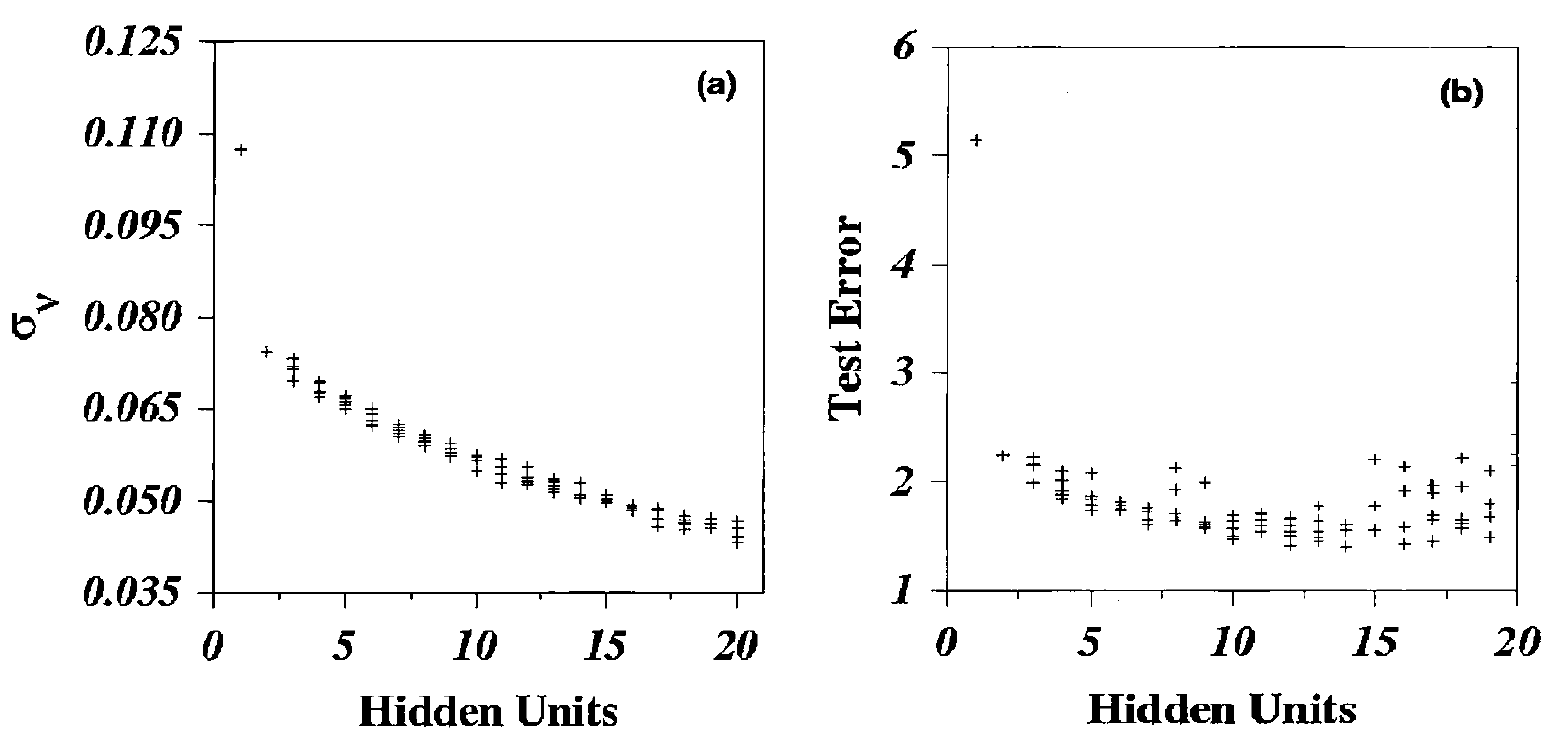
\includegraphics[scale=0.35]{images/vhn-test-error-plot.png}
	\caption {
		 Po lewej wykres zależności poziomu szumu od liczby neuronów w warstwie ukrytej, po prawej wykres zależności błedu predykcji od liczby neuronów w warstwie ukrytej, wykresy pochodzą z pracy \cite{doi:10.1080/13640461.2003.11819537}
	}
	\label{fig:vhn-pred-mae-plot}
\end{figure}

Dalsze badania były oparte na budowie komitetu modeli, w którym wynik przedstawiony był jako średnia wartość predykcji modeli wchodzących w jego skład. Badane komitety były budowane z modeli, które osiągały najlepsze wyniki w badaniach liczby neuronów oraz stałych regularyzacji. Wyniki badania zostały przedstawione na rys. \ref{fig:committee-plot}. Badacze stwierdzili, że najlepszym komitetem okazał się ten składający się z 10 najlepszych modeli, co widać na wyżej wspomnianym rysunku.

\begin{figure}[ht]{}
	\centering
	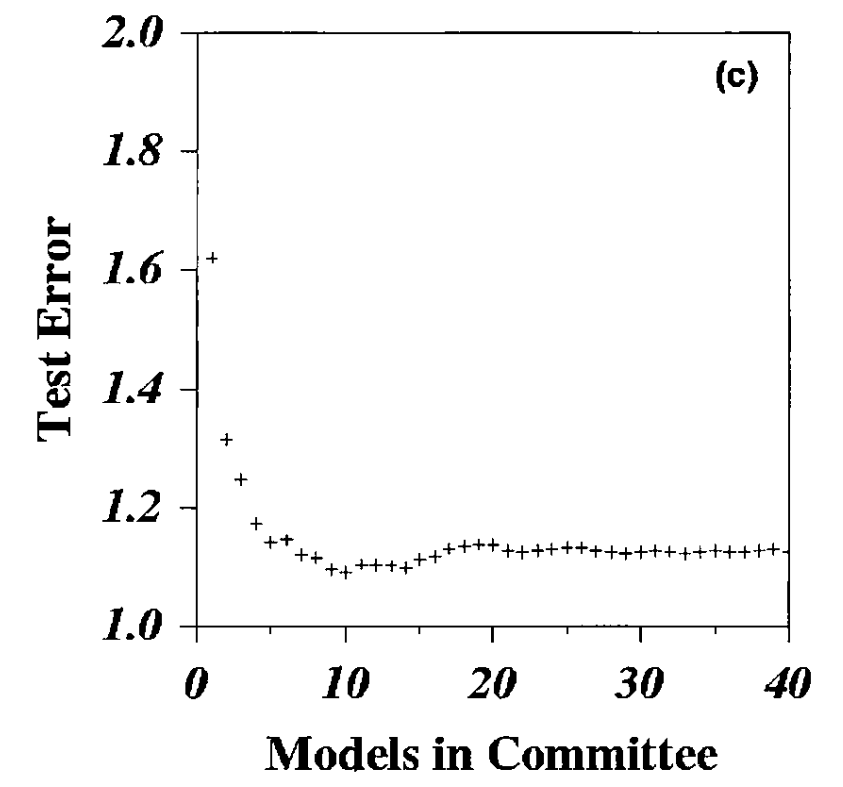
\includegraphics[scale=0.35]{images/committee-plot.png}
	\caption {
		 Wykres zależności błędu predykcji od liczby modeli wchodzących w skład komitetów \cite{doi:10.1080/13640461.2003.11819537}
	}
	\label{fig:committee-plot}
\end{figure}

Budowa modeli predykcyjnych twardości została także przedstawiona w pracach \cite{POURASIABI2012782}, \cite{10.1007/978-3-030-36802-9_43}, \cite{10.1007/978-3-030-36802-9_44}, gdzie prace \cite{10.1007/978-3-030-36802-9_43} i \cite{10.1007/978-3-030-36802-9_44}, autorów Savagounder'a, Patra i Bornanda, zostały opublikowane równolegle, bazując na danych, które zostały przedstawione w \cite{POURASIABI2012782}. Wspomniany zbiór danych zawiera 96 próbek zróżnicowanych pod względem składu chemicznego oraz parametrów obróbki cieplnej. Został on sporządzony na podstawie badań twardości żeliwa ADI, których procedura została ściśle opisana w artykule.

W pracy Hamida oraz Hameda PourAsiabi i innych \cite{POURASIABI2012782}, model predykcyjny został opracowany w sposób przedstawiony na rys. \ref{fig:sch-vhn-pourasiabi}. Jest to model sieci neuronowej, w~której warstwa wejściowa składa się z: wartości proc. miedzi i molibdenu oraz temperatury i czasu ausferrytyzacji. Warstwa ukryta składa się z 5 neuronów, w której funkcją aktywacji jest funkcja tangensoidalna. Zbiór danych został podzielony na zbiór treningowy oraz testowy w proporcji 70/26. Do minimalizacji błędu sieci została użyta metoda błędu średniokwadratowego, a dla uzyskania optymalnych wag został użyty algorytm Levenberga-Marquardta, bazujący na pochodnej drugiego rzędu funkcji błędu. Została także zastosowana normalizacja wymiarów wejściowych do wartości z zakresu [-1,1].


\begin{figure}[ht]{}
	\centering
	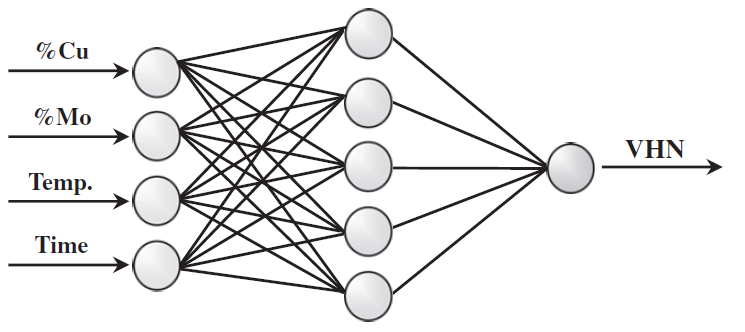
\includegraphics[scale=0.5]{images/model_vhn_pourasiabi.png}
	\caption {
		 Schemat modelu sieci neuronowej przedstawionego w pracy \cite{POURASIABI2012782}.
	}
	\label{fig:sch-vhn-pourasiabi}
\end{figure}

Wyniki testów wytrenowanej sieci neuronowej zostały przedstawione za pomocą współczynnika korelacji, którego wartość wyniosła 0.9912. Tak wysoki wynik świadczy o~dobrze wytrenowanej sieci oraz zdolności do poprawnego przewidywania twardości.

% \cite{adi-pred-2006}
% \cite{adi-pred-2014}

% \subsection{Inne wybrane modele predykcyjne}
% \label{sec:other-pred}
% \cite{ai_heat_treatment}
% \cite{GUO201995}
% \cite{4344283}

\section{Opis wybranych algorytmów heurystycznych}
W tej sekcji zostały przedstawione algorytmy heurystyczne, ktore zostały użyte na potrzeby optymalizacji parametrów produkcji żeliwa ADI (sekcja \ref{sec:algos}). Należą one do rodziny algorytmów przeszukiwania lokalnego ze względu na wykorzystanie sąsiedztwa wartości parametrów.

\subsection{Hill Climbing i Stochastic Hill Climbing}
Algorytm Hill Climbing \cite{hillclimbing} jest algorytmem przeszukiwania lokalnego zachłannego (nazywany też wspinaniem wzdłuż gradientu). Dla aktualnego rozwiązania wybierany jest zawsze sąsiad z największą bądź najmniejszą wartością funkcji celu w zależności od czego czy rozpatrywany jest problem minimalizacji bądź maksymalizacji. Wadą tego algorytmu jest zatrzymywanie się w w minimach/maksimach lokalnych. Algorytm Stochastic Hill Climbing jest modyfikacją poprzedniego algorytmu, która dokłada losowość. W tym algorytmie następne rozpatrywane rozwiązanie jest losowane z dostępnych sąsiadów do póki któryś z nich nie okaże się lepszy od aktualnego. Algorytm nie posiada określonego kryterium stopu więc należy zastosować np. maksymalny czas przeszukiwania bądź maksymalną liczbę kroków.

\subsection{Tabu Search}
Algorytm Tabu Search \cite{tabusearch} realizuje mechanizm, który nie pozwala zatrzymywać się przeszukiwaniu w ekstremach lokalnych. Oparty jest na redukcji przestrzeni przeszukiwań o znalezione rozwiązania. Podczas działania algorytmu używana jest tablica tabu, która na początku jest pusta. Do tablicy dodajemy rozwiązanie, które okazuje się gorsze od wybranego sąsiada. Zbiór wygenerowanych sąsiadów jest w każdym kroku algorytmu uszczuplany o rozwiązania znajdujące się w tablicy tabu. Rozwiązania są usuwane z tablicy tabu po pewnej określonej liczbie iteracji. Nie posiada on naturalnego warunku zakończenia. Wadą tego algorytmu jest przetrzymywanie w pamięci tablicy tabu.

Algorytm Tabu Search można zaimplementować na dwa sposoby:
\begin{itemize}
    \item uniemożliwienie generowania nowych rozwiązań, które są w tablicy tabu,
    \item nowe rozwiązanie nie może zostać wybrane, jeśli znajduje się w tablicy tabu.
\end{itemize}

Złamanie tablicy tabu dopuszczalne jest w przypadku, gdy wszyscy sąsiedzi danego rozwiązania znajdują się w tablicy tabu.

\subsection{Metropolis Search}
Algorytm Metropolisa \cite{metropolis} jest algorytmem statystycznego symulowania zmian ciała stałego w gorącej kąpieli aż do stanu termicznej równowagi. Przeszukiwanie odbywa się w następujący sposób:
\begin{itemize}
    \item dla danego rozwiązania \textit{i} wykonujemy statystyczny 'ruch' cząstki, otrzymując rozwiązanie \textit{j},
    \item jeżeli $E_{j}-E_{i} < 0$ (E - energia rozwiązania) to wybieramy rozwiązanie \textit{j},
    \item w przeciwnym wypadku wybieramy rozwiązanie \textit{j} z prawdopodobieństwiem \\* $exp\Big(-\frac{E_{j}-E_{i}}{k_{b}T}\Big)$
    \item wykonujemy kolejny statystyczny 'ruch'.
\end{itemize}

Algorytm nie posiada kryterium stopu, należy zastosować maksymalny czas bądź maksymalną liczbę kroków.

\section{Algorytmy heurystyczne w optymalizacji pro\-ce\-su pro\-du\-kcji}

Pierwszą z omówionych prac jest praca autorstwa A. Kumara i innych \cite{doi:10.1002/srin.201100189}, w której została zastosowana optymalizacja Pareto przy użyciu algorytmów genetycznych w oparciu o zbiór danych. Przedmiotem optymalizacji były właściwości mechaniczne stali mikrostopowej, a dokładniej: wytrzymałość na rozciąganie, wydłużenie oraz granica plastyczności. Na potrzeby optymalizacji zostały stworzone modele właściwości mechanicznych oparte na ewolucyjnych sieciach neuronowych (EvoNN). W pracy została przeprowadzona optymalizacja wielokryterialna oparta na optymalizacji następujących zestawów kryteriów:
\begin{itemize}
    \item maksymalizacji wytrzymałości na rozciąganie oraz granicy plastyczności,
    \item maksymalizacji granicy plastyczności oraz wydłużenia,
    \item maksymalizacji granicy plastyczności oraz minimalizacji stosunku granicy plastyczności do wytrzymałości na rozciąganie.
\end{itemize}
Trzy powyższe zadania optymalizacji zostały przeprowadzone z użyciem wielo-kryterialnego algorytmu genetycznego o nazwie 'predator-prey'. Rozwiązania Pareto dla każdego z zadań optymalizacyjnych odbiegały znacząco od rozwiązań opartych na danych użytych do budowy modeli. Aby sprawdzić tę bardzo istotną obserwację, przygotowano stop w bliskim sąsiedztwie kompozycji uzyskanej z frontu Pareto, która zgodnie z wiedzą badaczy nie była do tej pory przez nikogo badana. Próbki pochodzące z przygotowanego stopu zostały zbadane i ich właściwości (w granicy błędów eksperymentalnych) były całkiem zgodne z frontem Pareto. Badacze ocenili, że stworzenie stali o lepszych kombinacjach właściwości niż którykolwiek z elementów ze zbioru danych byłoby niemożliwe do uzyskania poprzez wykonanie samych eksperymentów, a udało się uzyskać taką kombinację za pomocą optymalizacji wielokryterialnej.

Następną z prac omawiających optymalizację procesu produkcji jest praca autora R. Radisa i innych \cite{radivsa2017casting}, w której badacze podjeli się problemu optymalizacji geometrii podajnika służącego do odlewania łyżki turbiny Peltona. Utworzona funkcja celu została opracowana na podstawie wymogów transferu ciepła. Zostały także opracowane 4 różne wymagania dla rozwiązań zwracanych przez algorytmy optymalizacji. Optymalizacji zostały poddane 4 różne wartości (H, R, r, l) przy użyciu 4 różnych algorytmów metaheurystycznych: algorytmu genetycznego, kolonii mrówek, symulowanego wyżarzania i optymalizacji roju cząstek. Wyniki otrzymane dla każdego z algorytmów okazały się bardzo zbliżone do siebie. Na ich podstawie został zamodelowany podajnik dla którego zostały przeprowadzone symulacje numeryczne potwierdzające poprawność rozwiązania.

    
\chapter{Koncepcja rozwiązania} \label{chap:methodology}

\section{Opis problemu}
\label{sec:problemDescription}
Problemem do rozwiązania dla zaimplementowanego systemu będzie podejmowanie decyzji w związku z wartościami parametrów produkcji odlewanego detalu biorąc pod uwagę:
\begin{itemize}
    \item spełnienie wymaganej jakości dla danego zamówienia,
    \item uzyskanie jak najmniejszego kosztu produkcji,
    \item zwiększenie wiarygodności parametrów zwracanych przez system na podstawie preferencji użytkownika.
\end{itemize}

Wymaganą jakość dla danego zamówienia określa norma EN-PN 1564:2012 \cite{pnen1564} (rys. \ref{fig:en-pn-1564}). Zawarte są w niej właściwości fizyczne stopów ADI w odniesieniu do oznaczeń, jakie są używane w przekazywanych informacjach między odlewnią a jej klientami.
\begin{figure}[ht]{}
	\centering
	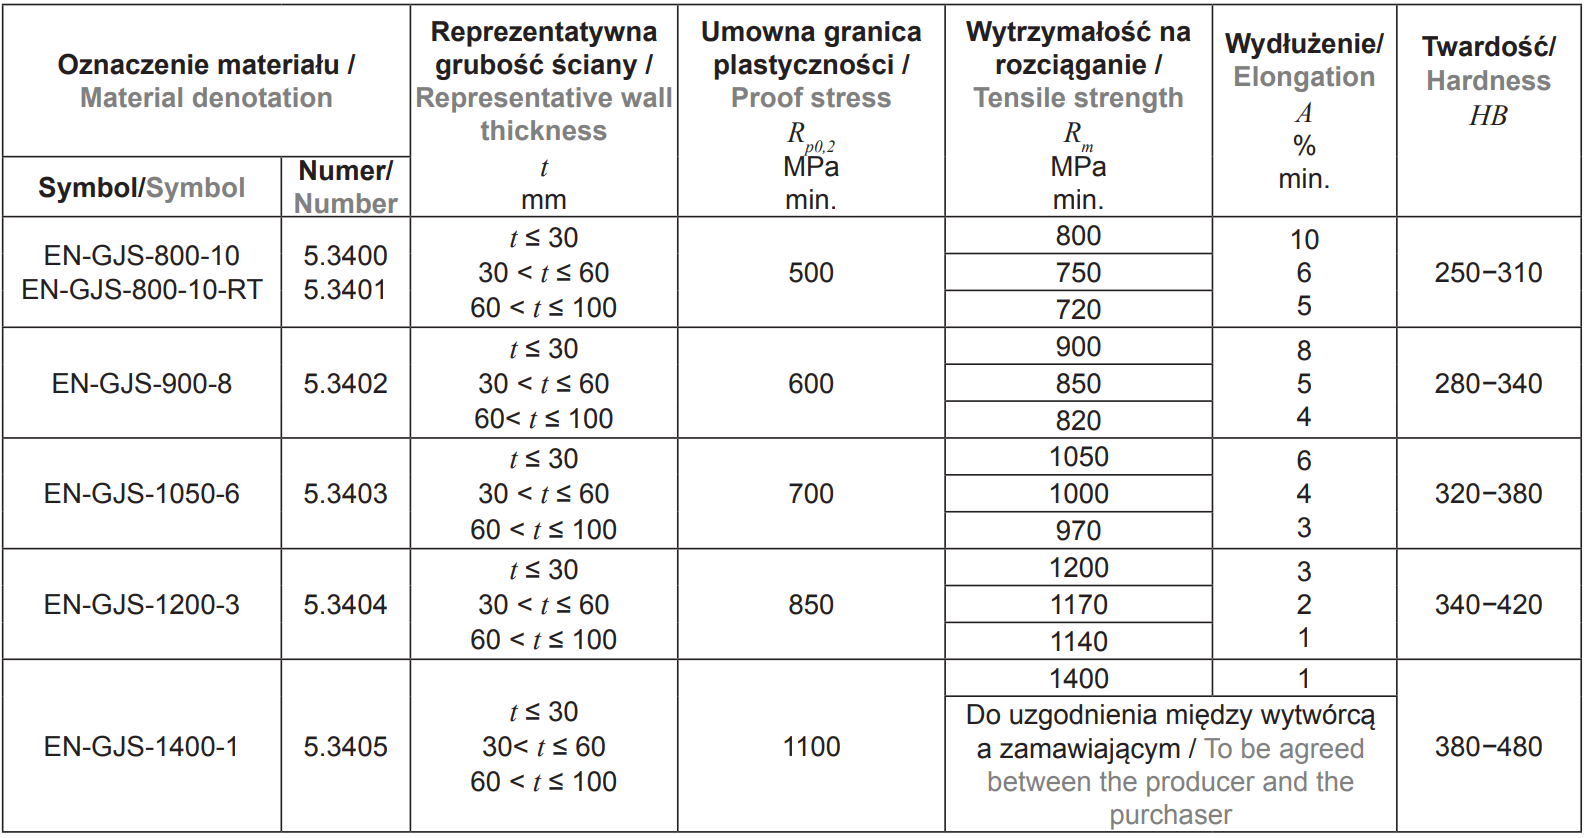
\includegraphics[scale=0.35]{images/en-pn-1564.PNG}
	\caption {
		 Właściwości mechaniczne żeliwa ADI wg PN-EN 1564:2012.
	}
	\label{fig:en-pn-1564}
\end{figure}

W celu lepszego zrozumienia sposobu pracy odlewni zostały sporządzone diagramy obrazujące w uproszczony sposób jak wygląda proces produkcji w takim zakładzie (rys. \ref{fig:schemat_linii}).
\begin{figure}[ht]{}
	\centering
	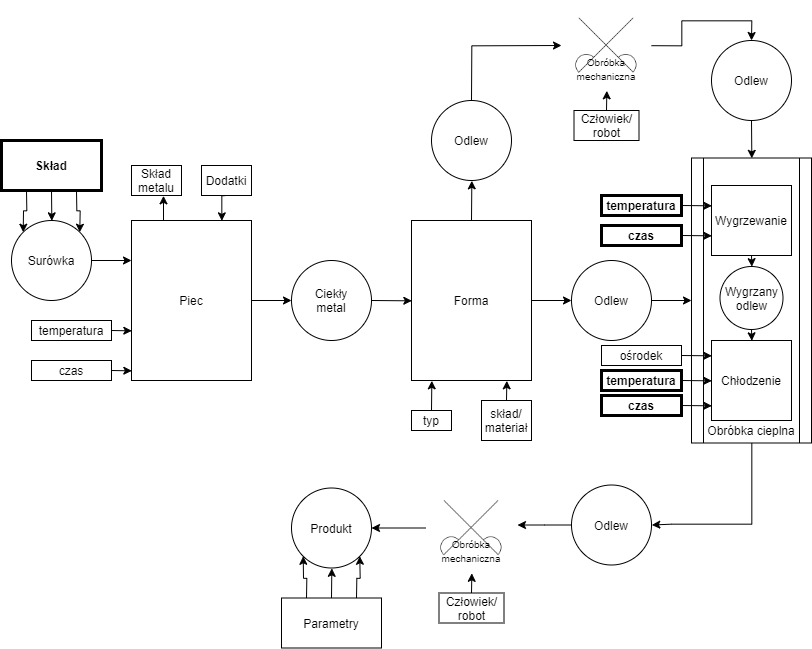
\includegraphics[scale=0.4]{images/schemat_prod.png}
	\caption {
		 Schemat linii producyjnej odlewni wytwarzającej żeliwo ADI.
	}
	\label{fig:schemat_linii}
\end{figure}
Realizacja zamówień produkcyjnych odbywa się poprzez wysłanie przez zleceniodawcę zapytania ofertowego, w którym zawarte są następujace elementy:
\begin{itemize}
    \item rysunek techniczny, a na nim:
    \begin{itemize}
        \item masa detalu,
        \item chropowatość,
        \item gatunek stopu,
        \item stosowane normy, odstępstwa.
    \end{itemize}
    \item liczba sztuk/elementów,
    \item spodziewany czas realizacji,
    \item warunki odbioru,
    \item zakres obróbki mechanicznej,
\end{itemize}
Z wyżej wymienionych elementów praca będzie się skupiała na:
\begin{itemize}
    \item masie detalu,
    \item gatunku stopu,
    \item stosowanych normach,
    \item liczbie sztuk detalu.
\end{itemize}
Powyższe elementy zostały wybrane ze względu na bezpośredni związek z kosztami produkcji oraz ograniczeniami, do których należy się odnieść przy próbach wspomagania decyzji.

Przed uruchomieniem produkcji sporządzana jest oferta w oparciu o zapytanie ofertowe, która powstaje poprzez:
\begin{itemize}
    \item analizę mocy przerobowej,
    \item analizy konstruktora lub/i technologa czy zasoby jakimi dysponuje odlewnia umożliwiają wykonanie detalu zgodnie z wytycznymi i dostarczonym rysunkiem,
    \item szacowanie kosztów.
\end{itemize}

W ramach zaimplementowanego systemu będą rozpatrywane następujące procesy produkcji:
\begin{itemize}
    \item proces planowania -> zebranie informacji o detalu, który ma zostać wykonany,
    \item proces przygotowania wsadu -> ustalenie \% mas pierwiastków w odlewanym stopie,
    \item austenityzacja, hartowanie izotermiczne -> temperatury i czasy trwania procesów austenityzacji i ausferryzacji.

\end{itemize}

\section{Budowa modelu predykcyjnego}
\label{sec:model}
W celu zbudowania przestrzeni rozwiązań, w której będą mogły poruszać się algorytmy optymalizacyjne, zachodzi potrzeba stworzenia modelu predykcyjnego właściwości mechanicznych. Zadaniem tego modelu będzie przewidywanie właściwości mechanicznych żeliwa ADI na podstawie:
\begin{itemize}
    \item składu chemicznego odlewu, w którym wyróżniamy następujące parametry (wartości procentowe):
    \begin{itemize}
        \item C - węgiel,
        \item Si - krzem,
        \item Mn - mangan,
        \item Mg - magnez,
        \item Cu - miedź,
        \item Ni - nikiel,
        \item Mo - molibden,
        \item S - siarka,
        \item P - fosfor,
        \item Cr - chrom.
    \end{itemize}
    \item grubości odlewu (wartość w milimetrach),
    \item parametrów obróbki cieplnej:
    \begin{itemize}
        \item temperatura austenityzacji (stopnie Celsjusza),
        \item czas austenityzacji (minuty),
        \item temperatura ausferrytyzacji (stopnie Celsjusza),
        \item czas ausferrytyzacji (minuty).
    \end{itemize}
\end{itemize}
Wartościami przewidywanymi przez model będą:
\begin{itemize}
    \item R\textsubscript{m} - wytrzymałość na rozciąganie [MPa],
    \item R\textsubscript{p0,2} - granica plastyczności [MPa],
    \item A5 - wydłużenie [\%],
    \item HB - twardość w skali Brinella [HB],
    \item K - udarność [J].
\end{itemize}

Model zostanie zbudowany na podstawie danych zebranych z artykułów przedstawiających badania właściwości mechanicznych żeliwa ADI. Ze względu na trudność w~przeprowadzaniu badań części właściwości mechanicznych, w wielu próbkach będą występowały braki danych. Sposób na ustalenie brakujących wartości został przedstawiony w~pracy \cite{Kochanski12}. Zakłada się, że w pracy zostaną przeprowadzone badania nad następującymi algorytmami uczenia maszynowego, które mogą posłużyć do budowy wspomnianych modeli:
\begin{itemize}
    \item Random Forest,
    \item Gradient Boosting,
    \item Multilayer Perceptron,
    \item Ensemble Averaging.
\end{itemize}

\section{Funkcja kosztu}
W celu opracowania funkcji kosztu został sporządzony diagram obrazujacy zależności parametrów odlewu oraz jego obróbki cieplnej od ceny i właściwości fizycznych wytopu (rys. \ref{fig:parametry}). 
\begin{figure}[H]{}
	\centering
	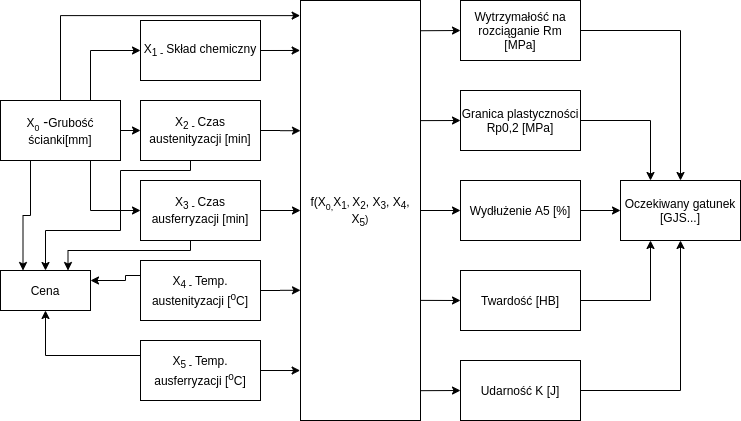
\includegraphics[scale=0.45]{images/parametry_produkcji.png}
	\caption {
		 Diagram zależności między parametrami odlewu oraz obróbki cieplnej od właściwości fizycznych odlewu oraz wpływu na cenę detalu.
	}
	\label{fig:parametry}
\end{figure}

Na diagramie znajduje się blok przedstawiający model predykcyjny\linebreak$f(X_{0},X_{1},X_{2},X_{3},X_{4},X_{5})$, (parametry $X_{i}$ zostały opisane na diagramie), który ma za zadanie przewidywać właściwości mechaniczne wyrobu. Zakłada się, że możliwe jest stworzenie takiego modelu, dzięki któremu będzie możliwe otrzymywanie informacji o gatunku żeliwa dla wybranych parametrów procesu produkcji odlewu. Wzorując się na wymiarach wejściowych modeli przedstawionych w \cite{YESCAS2001162}, czas ausferrytyzacji zostanie także przedstawiony jako wartość logarytmu o podstawie 10 z wartości czasu w sekundach.

Bazując na przygotowanych przez ekspertów tabelach opisujących wpływ poszczególnych parametrów wytopu na cenę gotowego detalu (zakładając wagę detalu 1kg), została opracowana funkcja kosztu:

\begin{equation}
   C(CC, HTP) = \Big(1+cost\_inc\_cc(CC) + \sum_{htp \in HTP} cost\_inc\_htp(htp)\Big) \cdot avg\_iron\_cost 
\end{equation}
gdzie:
\begin{itemize}
    \item \textit{CC} (chemical composition) - zbiór parametrów składu chemicznego wytopu
    \item \textit{HTP} (heat treatment parameters) - zbiór parametrów obróbki cieplnej, który zawiera następujące elementy:
    \begin{itemize}
        \item temperatura austenityzacji,
        \item czas austenityzacji,
        \item temperatura ausferrytyzacji,
        \item czas ausferrytyzacji,
    \end{itemize}
    \item \textit{cost\_inc\_cc} (cost increase) - funkcja zwracająca procent wzrostu kosztu w zależności od składu chemicznego (dokładnie od zawartości niklu, miedzi i molibdenu),
    \item \textit{cost\_inc\_htp} (cost increase) - funkcja zwracająca procent wzrostu kosztu w zależności od wartości parametru obróbki termicznej,
    \item \textit{avg\_iron\_cost} (average iron cost) - średnia cena żeliwa sferoidalnego,
    \item \textit{htp} - parametr ze zbioru parametrów obróbki cieplnej np. temp. austenityzacji, 880\degree C,
    \item \textit{base\_cost} - koszt bazowy np. 61 zł.
\end{itemize}

\section{Funkcja jakości}
Przegląd różnych badań właściwości żeliwa ADI pokazuje, że badania te często są przeprowadzane w postaci eksperymentów, w~których eksplorowane są niestosowane w masowej produkcji zestawy parametrów. Takie zestawy parametrów mogą być uważane za mało wiarygodne przez użytkownika systemu. W tym celu zaproponowana została funkcja określająca jakość parametrów dla zdefiniowanych przez użytkownika nominalnych zakresów prametrów oraz wag tych parametrów. Wartość takiej funkcji będzie określała jak bardzo parametry zwrócone przez system są zgodne z oczekiwaniami użytkownika. Funkcja została zdefiniowana w następującej postaci:
\begin{equation}
     Q(P) = \sum_{p \in P} \big(in\_range(p) \cdot w_p\big) 
\end{equation}

gdzie:
\begin{itemize}
    \item \textit{P} - zbiór parametrów produkcji (skład chemiczny, obróbka cieplna)
    \item \textit{p} - parametr ze zbioru P
    \item \textit{in\_range} - funkcja określająca, czy wartość danego parametru mieści się w przedziale zdefiniowanym przez użytkownika
    \item \textit{w\textsubscript{p}} - waga parametru p, zdefiniowana przez użytkownika
\end{itemize}

\section{Optymalizacja heurystyczna}\label{sec:heur-opt}
W pracy zakładane jest użycie różnych algorytmów heurystycznych z dziedziny optymalizacji jednokryterialnej. Zachodzi także potrzeba zdefiowania zbioru parametrów, które będą eksplorowane za pomocą algorytmów.

\subsection{Zbiór parametrów}\label{sec:param_set}
Budowa zbioru parametrów produkcji będzie opierać się na:
\begin{itemize}
    \item przyjętych przez wytwórców żeliwa możliwych zmianach parametrów obróbki cieplnej tj. zmiany temperatur o +/- 5 stopni Celsjusza, zmiany czasów o +/- 15 minut,
    \item założeniu, że zbiór składów chemicznych jest skończony i ograniczony do składów, które wystąpiły w trakcie uczenia i testowania modelu predykcyjnego oraz składów wprowadzonych przez użytkownika,
    \item minimalnych i maksymalnych wartości parametrów produkcji, jakie wystąpiły podczas uczenia i testowania modelu predykcyjnego.
\end{itemize}

\subsection{Optymalizacja jednokryterialna}\label{sec:opt}
W przypadku użycia algorytmów optymalizacji jednokryterialnej zachodzi potrzeba sprowadzenia zdefiniowanych poprzednio kryteriów tj. kosztu i jakości, do jednego kryterium. Jednym ze sposobów na dokonanie takiego sprowadzenia, jest użycie skalaryzacji ważonej, która polega na znormalizowaniu wartości kryteriów do takiego samego zakresu wartości np. [0,1], a następnie zsumowaniu tych wartości przemnożonych przez wagi tych kryteriów.

W takim podejściu zostanie przyjęte, że to użytkownik wprowadza wagi kryteriów optymalizacyjnych. Problem skalaryzacji ważonej dla znormalizowanych kryteriów ceny i~jakości wygląda następująco:
\begin{equation}
     \min_{(CC,HTP) \in X} QC\Big(C\_norm(CC,HTP),1-Q\_norm(CC \cup HTP),\theta\Big) 
\end{equation}
gdzie:
\begin{itemize}
    \item CC - zbiór parametrów składu chemicznego wytopu,
    \item HTP - zbiór parametrów obróbki cieplnej,
    \item X - zbiór wszystkich możliwych parametrów,
    \item C\_norm - znormalizowana wartość funkcji kosztu,
    \item Q\_norm - znormalizowana wartość funkcji jakości,
    \item $\theta$ - zbiór wag kryteriów kosztu i jakości ,
    \item QC - funkcja następującej postaci:
    \begin{equation}
        QC(X_1, X_2, \theta) = X_1\cdot\theta(X_1) + X_2\cdot\theta(X_2)
    \end{equation}
\end{itemize}

Przedstawiony powyżej problem polega na minimalizacji funkcji QC dla parametrów produkcji. Aby rozwiązania znajdowane przez algorytm były poprawne, należy wprowadzić ograniczenia wynikające z gatunku wymaganego przez klienta. Są one zdefiniowane we wspomnianej już wcześniej normie EN-PN 1564, w której znajdują się minimalne (i~ maksymalne dla twardości) wartości właściwości mechanicznych w zależności od oczekiwanej grubości detalu. 

W celu sprawdzenia, czy dla danych parametrów produkcji otrzymamy oczekiwane przez normę wartości mechaniczne, użyty zostanie zbudowany model predykcyjny opisany w podrozdziale  \ref{sec:model}. Model dla podanych parametrów zwróci przewidywane właściwości mechaniczne i na ich podstawie możliwe będzie sprawdzenie, czy będą one spełniały warunki wymagane przez normę.

\subsection{Wybrane algorytmy i metodologia ich porównania}\label{sec:algos}
Dla celów badawczych zostaną wybrane różne algorytmy heurystyczne służące do optymalizacji jednokryterialnej.

W celu porówniania działania algorytmów, zostanie przeprowadzony test polegający na przeprowadzeniu procesu optymalizacji dla różnych ograniczeń czasowych, w których mierzone i porównywane będą następujace wartości:
\begin{itemize}
    \item liczba przeliczeń funkcji QC,
    \item liczba przewidywań wartości właściwości mechanicznych, które w rezultacie będą eliminować wybrane parametry,
    \item najniższą wartość funkcji QC.
\end{itemize}

\subsubsection{Algorytmy optymalizacji jednokryterialnej}
Do przeprowadzenia badań w kontekście optymalizacji jednokryterialnej zostały wybrane algorytmy z dziedziny lokalnego przeszukiwania:
\begin{itemize}
    \item Stochastic Hill Climbing - stochastyczne wspinanie,
    \item Hill Climbing - podstawowa wersja wspinania,
    \item Tabu search,
    \item Metropolis search,
    \item Parallel tempering - współbieżne szukanie za pomocą wielu instancji Metropolis Search z różnymi temperaturami.
\end{itemize}

% \section{System agentowy}
% \label{system_agentowy}
% Na potrzeby wspomagania decyzji zostanie stworzony system agentowy o koncepcyjnej strukturze znajdujacej się na rys. \ref{fig:system_agentowy}.

% \begin{figure}[h]{}
% 	\centering
% 	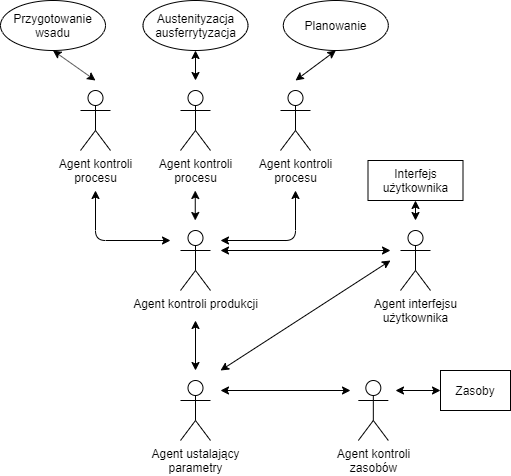
\includegraphics[scale=0.6]{images/system_agentowy.png}
% 	\caption {
% 		 Koncepcyjny schemat systemu agentowego na potrzeby wspomagania decyzji.
% 	}
% 	\label{fig:system_agentowy}
% \end{figure}

% Na schemacie można wyróżnić następujące elementy:
% \begin{itemize}
%     \item procesy, a w nich:
%     \begin{itemize}
%         \item \textbf{proces planowania} - w trakcie trwania tego procesu zbierane są dane o wymaganiach co do realizowanego zamównienia (masa detalu, ilość sztuk, wymagany gatunek) przez agenta kontroli procesu
%         \item \textbf{proces obróbki cieplnej} (austenityzacja, ausferrytyzacja) - wykonywany dla danych dostarczonych przez agenta kontroli procesu (temperatury i czasy trwania poszczególnych etapów obróbki)
%         \item \textbf{proces przygotowania wsadu} - wykonywany dla danych dostarczonych przez agenta kontroli procesu (skład wytopu)
%     \end{itemize}
%     \item agenci, a w nich:
%     \begin{itemize}
%         \item \textbf{Agent kontroli procesu} - agent zajmujący się bezpośrednią komunikacją z procesem (zbiera lub dostarcza dane)
%         \item \textbf{Agent kontroli produkcji} - agent zajmujący się kontrolą produkcji poszczególnych procesów i zarządzaniem danych, które od nich otrzymuje.
%         \item \textbf{Agent interfejsu użytkownika} - agent zajmujący się komunikacją z: użytkownikiem poprzez interfejs użytkownika; agentem kontroli produkcji; agentem ustalającym parametry
%         \item \textbf{Agent ustalający parametry} - na podstawie informacji ustalonych podczas procesu planowania, przeszukuje za pomocą algorytmów heurystycznych przestrzeń rozwiązań w celu zminimalizowania kosztu przy jednoczesnym spełnieniu wymaganej jakości
%         \item \textbf{Agent kontroli zasobów} - agent dostarczający informację o dostępnych zasobach (ilości składowych wytopów, możliwych czasach użycia pieców służących do obróbki cieplnej).
%     \end{itemize}
%     \item elementy zewnętrzne:
%     \begin{itemize}
%         \item interfejs użytkownika
%         \item zasoby
%     \end{itemize}
% \end{itemize}

\section{Koncepcja wspomagania decyzji}\label{sec:dec-sup-sys-concept}
Założone zostało stworzenie systemu wykorzystującego opisane powyżej elementy, tj, optymalizacja kryteriów jakości i kosztu oraz modele predykcyjne, dla potrzeb wspomagania decyzji o wyborze składu wytopu oraz parametrów obróbki cieplnej dla żądanego gatunku oraz określonych zakresów wiarygodności parametrów. 

Użytkownik systemu będzie miał za zadanie wprowadzać niezbędne informacje za pomocą interfejsu graficznego. Informacjami wprowadzanymi przez użytkownika będą:
\begin{itemize}
    \item wymagany gatunek odlewu,
    \item grubość odlewu,
    \item liczba sztuk detalu oraz jego waga,
    \item wagi kryteriów kosztu i jakości,
    \item zakresy wiarygodności parametrów oraz ich wagi,
    \item maksymalny czas szukania rozwiazania.
\end{itemize}
Dodatkowymi parametrami związanymi z wyliczaniem wartości funkcji kosztu są:
\begin{itemize}
    \item ceny niklu, miedzi, molibdenu,
    \item średnia cena żeliwa ADI.
\end{itemize}
W odpowiedzi system będzie zwracał rozwiązanie zawierające następujące informacje:
\begin{itemize}
    \item skład chemiczny wytopu,
    \item parametry obróbki cieplnej,
    \item wartość funkcji kosztu,
    \item wartość funkcji jakości.
\end{itemize}

Została opracowana abstrakcyjna architektura omówionej koncepcji systemu. Jej schemat został przedstawiony na rysunku \ref{fig:abst-arch}. Dla przejrzystości tego schematu, pominięte zostały opisy danych przekazywanych między obiektami systemu.
\begin{figure}[ht]{}
	\centering
	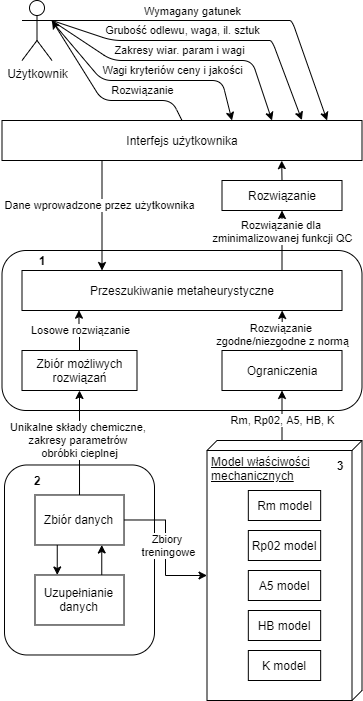
\includegraphics[scale=1]{images/system_wspomagania_decyzji-new.png}
	\caption {
		 Abstrakcyjna architektura systemu wspomagania decyzji.
	}
	\label{fig:abst-arch}
\end{figure}

\FloatBarrier

Opis bloków przedstawionych na rys. \ref{fig:abst-arch}:
\begin{itemize}
    \item Interfejs użytkownika - warstwa oddzielająca użytkownika od systemu za pomocą której użytkownik będzie w stanie wprowadzić dane niezbędne do przeprowadzenia czynności skutkujących dostarczeniem rozwiązania/rozwiązań,
    \item Blok nr 1:
    \begin{itemize}
        \item Przeszukiwanie metaheurystyczne - moduł odpowiedzialny za przeszukiwanie przestrzeni rozwiązań w celu optymalizacji parametrów produkcji poprzez minimalizację funkcji QC,
        \item Zbiór możliwych rozwiązań - element systemu zawierający składowe pozwalające na zbudowanie przestrzeni rozwiązań, która zostanie użyta przez moduł przeszukiwania, 
        \item Ograniczenia - reprezentują wymagania jakie narzuca norma na właściwości mechaniczne wytopu, który byłby wytworzony korzystając z rozwiązania zwracanego przez system.
    \end{itemize}
    \item Blok nr 2:
    \begin{itemize}
        \item Zbiór danych - dane zebranych z artykułów,
        \item Uzupełnianie danych - moduł umożliwiający uzupełnienie brakujących danych w zbiorze danych. 
    \end{itemize}
    \item Model właściwości mechanicznych (blok nr 3) - dostarcza wartości właściwości mechanicznych dla danego rozwiązania,
    \item Rozwiązanie - reprezentuje odpowiedź, jaka zostanie zwrócona użytkownikowi (może zawierać zarówno jedno jak i wiele rozwiązań dla zminimalizowanej funkcji QC).
\end{itemize}



% \bt

% \section{Method 1}

% \bt

% \section{Method 2}

% \bt 

% \section{Method 3}

% Some nice matrices...

% \begin{equation}
% 	A = \begin{bmatrix}
% 		1 &    &    &    &    &    &    & \\
% 		1 & -2 &  1 &    &    &    &    & \\
% 		  &  1 & -2 &  1 &    &    &    & \\
% 		  &    &  1 & -2 &  1 &    &    & \\
% 		  &    &    &  1 & -2 &  1 &    & \\
% 		  &    &    &    &  1 & -2 &  1 & \\
% 		  &    &    &    &    &    &  1 & \\
% 	\end{bmatrix}
% 	\hspace{1cm}
% 	B = \begin{bmatrix}
% 		0 \\
% 		4 \\
% 		4 \\
% 		4 \\
% 		4 \\
% 		4 \\
% 		0
% 	\end{bmatrix}
% \end{equation}

% Some nice diagrams...

% \newcommand{\cv}[1]{ % column vector
% 	$\begin{bmatrix} #1 \end{bmatrix}$
% }
% \newcommand{\Cv}[1]{ { \cv{#1} } } % shortcut for tree leaves
% \newcommand{\elim} { $\xrightarrow{E}$ }
% \newcommand{\merge} { $\xrightarrow{M}$ }
% \newcommand{\xtract} { $\xrightarrow{X}$ }

% \begin{figure}[H]
% 	\centering
% 	\caption{Elimination tree for multifrontal solver}
% 	\label{fig:mfs-elim-tree}
% 	\begin{forest}
% 		for tree = {
% 			draw,
% 			edge={<-, line width=2pt},
% 			minimum height=2cm,
% 			anchor=north,
% 			align=center,
% 			child anchor=north
% 		},
% 		[ { \merge \cv{x_1 \\ x_5 \\ x_7} \elim \cv{x_1 \\ x_7 } }
% 			[ { \merge \cv{x_1 \\ x_3 \\ x_5} \elim \cv{x_1 \\ x_5} }
% 				[ { \merge \cv{x_1 \\ x_2 \\ x_3} \elim \cv{x_1 \\ x_3} }
% 					[ \Cv{x_1 \\ x_2} ]
% 					[ \Cv{x_2 \\ x_3} ]
% 				]
% 				[ { \merge \cv{x_3 \\ x_4 \\ x_5} \elim \cv{x_3 \\ x_5} }
% 					[ \Cv{x_3 \\ x_4} ]
% 					[ \Cv{x_4 \\ x_5} ]
% 				]
% 			]
% 			[ { \merge \cv{x_5 \\ x_6 \\ x_7} \elim \cv{x_5 \\ x_7} }
% 				[ \Cv{x_5 \\ x_6} ]
% 				[ \Cv{x_6 \\ x_7} ]
% 			]
% 		]
% 	\end{forest}
% \end{figure}

% \pagebreak

% Some nice algorithms...

% \newcommand{\U}{\mathcal{U}}

% \begin{algorithm}
% \caption{One iteration of the double-grid algorithm}
% \label{alg:two-grid}

% \begin{algorithmic}

% 	\State Compute the solution $\U^C$ on the coarse mesh
% 	\State Split each element of the coarse mesh, thus obtaining the fine mesh
% 	\State Compute the solution $\U^F$ on the fine mesh

% 	\For{\textbf{each} coarse mesh element $\eps_i$}
% 		\LineComment{$\rho_i$ is the relative error}
% 		\State $ \rho_i \gets \left|
% 				\frac {
% 					\U^F_i - \U^C_i
% 				} {
% 					\U^F_i
% 				}
% 			\right| $
% 	\EndFor

% 	\State $\rho_{max} \gets$ $max_i(\rho_i)$

% 	\For{\textbf{each} element $\eps_i$}
% 		\If {$ \rho_i > \tau \cdot \rho_{max} $}
% 			\State adapt the $\eps_i$ element (split into two halves)
% 		\EndIf
% 	\EndFor

% \end{algorithmic}
% \end{algorithm}

% \pagebreak

% Some nice figures...

% \begin{figure}[H]
% 	\centering

% 	\caption[Double-grid h-adaptation strategy, steps 1-2] {
% 		Steps 1-5 of the double-grid h-adaptation strategy, quadratic B-splines
% 	}
% 	\label{fig:h-adapt-two-grid}

	

% 	\begin{subfigure}[h]{1.0\textwidth}
% 		\centering
% 		\includegraphics[scale=0.2]{frog.jpg}
% 		\caption{
% 			Step 2.
% 			Since the maximal error multiplied by $\tau$ (here set to 20\%) were lower than the error on any element,
% 			the algorithm halved all four elements after step 1.
% 		}
% 		\label{fig:h-adapt-two-grid-2}
% 	\end{subfigure}
% \end{figure}


% \begin{figure}[H]
% 	\ContinuedFloat % continue from previous page
% 	\caption[Double-grid h-adaptation strategy, steps 3-4]{} % for subcaption package to ensure proper numbering

% 	\begin{subfigure}[h]{1.0\textwidth}
% 		\centering
% 		\includegraphics[scale=0.2]{frog.jpg}
% 		\caption{
% 			Step 3.
% 			The extreme left and right elements did not get refined after the step 2.
% 		}
% 		\label{fig:h-adapt-two-grid-3}
% 	\end{subfigure}

% 	\begin{subfigure}[h]{1.0\textwidth}
% 		\centering
% 		\includegraphics[scale=0.2]{frog.jpg}
% 		\caption{
% 			Step 4
% 		}
% 		\label{fig:h-adapt-two-grid-4}
% 	\end{subfigure}
% \end{figure}




\chapter{Realizacja} \label{chap:realization}
W tym rozdziale zostały opisane realizacje elementów opisanych w koncepcji z rozdziału \ref{chap:methodology}. Ze względu na to, że realizacja części elementów została przeprowadzona z użyciem podobnych bądź tych samych narzędzi czy algorytmów, zostały one zagregowane i opisane w sekcji \ref{sec:tools}. W dalszych sekcjach zostały przedstawione kolejno:
\begin{itemize}
    \item proces zbierania i analizowania danych oraz próba uzupełnienia danych brakujących,
    \item budowa modeli predykcyjnych z wykorzystaniem różnych podejść i algorytmów,
    \item opis realizacji optymalizacji heurystycznej,
    \item prezentacja systemu wspomagania decyzji.
\end{itemize}

\section{Zbiór i opis narzędzi oraz algorytmów użytych podczas realizacji}\label{sec:tools}
\subsection{Analiza oraz modelowanie danych}\label{sec:tools-data-analysis-modeling}
Do tej części pracy zostały wykorzystane narzędzia, których miałem okazję użyć podczas projektów związanych z eksploracją danych oraz na zajęciach z uczenia maszynowego. Wybór został podyktowany niskim progiem wejścia lub ominięciem etapu poznawania nowych narzędzi.
\newpage
Lista użytych narzędzi:
\begin{itemize}
    \item Microsoft Office Excel\footnote{\url{https://www.microsoft.com/pl-pl/microsoft-365/excel}} - oprogramowanie użyte na potrzeby gromadzenia oraz edycji danych podczas budowy zbioru danych,
    \item Język programowania Python\footnote{\url{https://www.python.org/}} w wersji 3.7 - język interpretowany wysokiego poziomu, został wybrany ze względu na ogromną społeczność programistów oraz masę bibliotek wspomagających procesy analizy oraz modelowania danych,
    \item Jupyter Lab\footnote{\url{https://jupyter.org/}} - środowisko programistyczne dla języka Python uruchamiane w przeglądarce internetowej, umożliwia podzielenie kodu na komórki oraz wykonywanie ich wraz z prezentacją wyników,
    \item Pandas\footnote{\url{https://pandas.pydata.org/}} - narzędzie dla języka Python wspomagające analizę oraz manipulację danymi,
    \item Matplotlib\footnote{\url{https://matplotlib.org/}} - biblioteka dla języka Python umożliwiająca tworzenie wykresów,
    \item Scikit-learn\footnote{\url{https://scikit-learn.org/}} \cite{scikit-learn} - narzędzie dla języka Python dostarczające algorytmów służacych do budowy modeli uczenia maszynowego,
    \item TensorFlow\footnote{\url{https://www.tensorflow.org/}} \cite{tensorflow2015-whitepaper} - otwartoźródłowa platforma służąca do budowania modeli uczenia maszynowego, została wykorzystana do budowy sieci neuronowych ze względu na dobrze udokumentowany interfejs programistyczny Keras API\footnote{\url{https://keras.io/}} pozwalający na proste i szybkie definiowanie architektury modeli,
    \item XGBoost\footnote{\url{https://xgboost.ai/}} \cite{xgboost} -  biblioteka dostarczająca imlementację algorytmu gradient boostingu, która została zoptymalizowana pod kątem szybkości działania oraz jakości przewidywań, udostępnia API pozwalające używać jej z wykorzystaniem narzędzia scikit-learn.
\end{itemize}

Użyte algorytmy wraz ze skróconym opisem działania:
\begin{itemize}
    \item k-krotna walidacja krzyżowa \cite{crossvalidation} - metoda służąca do badania jakości wytrenowanych modeli poprzez podzielenie zbioru danych na k części i użycie jednego z podzbiorów jako zbioru testowego a pozostałych jako zbióe treningowy,
    \item Random Forest \cite{random_forest} - algorytm służący do budowania klasyfikatorów oraz regresorów  za pomocą ensemblingu drzew decyzyjnych, w którym każde z drzew jest budowane za pomocą próbkowania z podmianą ze zbioru treningowego,
    \item Gradient Boosting \cite{gradient_boosting} - algorytm służący do budowania klasyfikatorów oraz regresorów, w którym każdy kolejny model próbuje poprawić błędy predykcji poprzedniego,
    \item Ensemble Averaging \cite{ensemble_averaging} - proces tworzenia wielu różnych modeli i łączenia ich w jeden w celu poprawy jakości predykcji,
    \item Multilayer Perceptron \cite{negnevitsky2005artificial} - sieć neuronowa typu feed-forward, na ogół składająca się z warstwy wejściowej, jednej lub wielu warstw ukrytych i warstwy wyjściowej. Uczenie takiej sieci odbywa się przy użyciu algorytmu wstecznej propagacji błędu i stochastycznego spadku wzdłuż gradientu.
\end{itemize}

\subsection{Realizacja optymalizacji oraz budowa systemu wspomagania}
W tej części pracy zdecydowałem się na użycie narzędzi, z którymi miałem do czynienia podczas realizacji wielu projektów, zarówno komercyjnych jak i uczelnianych. Nabyte wcześniej doświadczenie umożliwiło sprawną ich konfigurację oraz rozwiązywanie napotkanych problemów.

Opis użytych narzędzi:
\begin{itemize}
    \item Język programowania Java w wersji 11 \footnote{\url{https://java.com/}} - wysokopoziomowy język programowania obiektowego, jeden z najpopularniejszych pod względem zastosowań komercyjnych. Został wybrany ze względu na wieloletnie doświadczenie związane z tworzeniem i rozwijaniem aplikacji komercyjnych i uczelnianych,
    \item OpenJFX \footnote{\url{https://openjfx.io/}} - biblioteka dla języka Java umożliwiająca tworzenie nowoczesnych interfejsów użytkownika. Ponownie, powodem wyboru było nabyte doświadczenie w realizacji projektów uczelnianych i komercyjnych,
    \item Maven \footnote{\url{http://maven.apache.org/}} - narzędzie służące do zarządzania zależnościami oraz budowaniem aplikacji w języku Java,
    \item IntelliJ IDEA \footnote{\url{https://www.jetbrains.com/idea/}} - zintegrowane środowisko programistyczne między innymi dla języka Java,
    \item JAMES Framework \footnote{\url{http://www.jamesframework.org/}} \cite{james} - nowoczesny framework dla języka Java udostępniający szereg algorytmów metaheurystyucznych z dziedziny przeszukiwania lokalnego (dokładny opis narzędzia znajduje się w sekcji \ref{sec:james}. Została wybrana ze względu na małe nakłady pracy potrzebne przy implementacji elementów potrzebnych do uruchomienia algorytmów znajdujących się w bibliotece,
    \item jMetal \footnote{\url{http://jmetal.github.io/jMetal/}} \cite{jmetal} - framework dla języka Java dostarczający szereg implementacji z dziedziny optymalizacji wielokryterialnej,
    \item DeepLearning4J \footnote{\url{https://deeplearning4j.org/}} - biblioteka dla języka Java, która została wykorzystana do używania wytrenowanych modeli za pomocą biblioteki TensorFlow.
\end{itemize}

Opis użytych algorytmów:
\begin{itemize}
    \item algorytmy optymalizacyjne z dziedziny lokalnego przeszukiwania:
        \begin{itemize}
            \item Random Descent - (znany również jako Stochastic Hill Climbing \cite{hillclimbing}) najprostszy algorytm lokalnego przeszukiwania polegający na generowaniu losowego sąsiada aktualnego rozwiązania i zapamiętywaniu tego, który jest od tego, który jest od aktualnego rozwiązania lepszy,
            \item Steepest Descent - (znany również jako Hill Climbing \cite{hillclimbing}) algorytm polegający na szukaniu i wybraniu najlepszego rozwiązania wśród sąsiadów aktualnego rozwiązania, jego działanie jest analogiczne do wspinania się w górę, co sugeruje sama nazwa,
            \item Tabu Search \cite{tabusearch} -  metaheurystyczny algorytm, który wykorzystuje tablicę o określonym rozmiarze w celu zapamiętywania najlepszych rozwiązań w danym sąsiedztwie,
            \item Metropolis Search - rozszerzenie algorytmu Random Descent za pomocą algorytmu opisanego w pracy \cite{metropolis}, gdzie rozwiązanie sąsiadujące, które nie jest lepsze od obecnego rozwiązania, może być zaakceptowane jako nowe rozwiązanie z pewnym prawdopodobieństwem. To prawdopodobieństwo jest związane z różnicą między wartościami ewaluacji rozwiązań oraz parametrem temperatury przeszukiwania (im wyższa tym prawdopodobieństwo jest wyższe). W bibliotece JAMES wartość tej temperatury jest nie zmienia się w trakcie przeszukiwania,
            \item Parallel Tempering \cite{paralleltempering} - algorytm polegający na współbieżnym uruchomieniu wielu instancji przeszukiwania za pomocą algorytmu Metropolis Search z~różnymi wartościami temperatury, 
            % \item NSGA-II \cite{nsgaii} - genetryczny algorytm wielokryterialnej optymalizacji
        \end{itemize}
\end{itemize}   

\subsubsection{Opis biblioteki JAMES}\label{sec:james}
Do użycia większości algorytmów znajdujących się w bibliotece należy wyspecyfikować problem do rozwiązania. Poszczególne elementy, które należy zdefiniować zostały przedstawione na rys. \ref{fig:james} pochodzącym z dokumentacji biblioteki JAMES. 

\begin{figure}[ht]{}
	\centering
	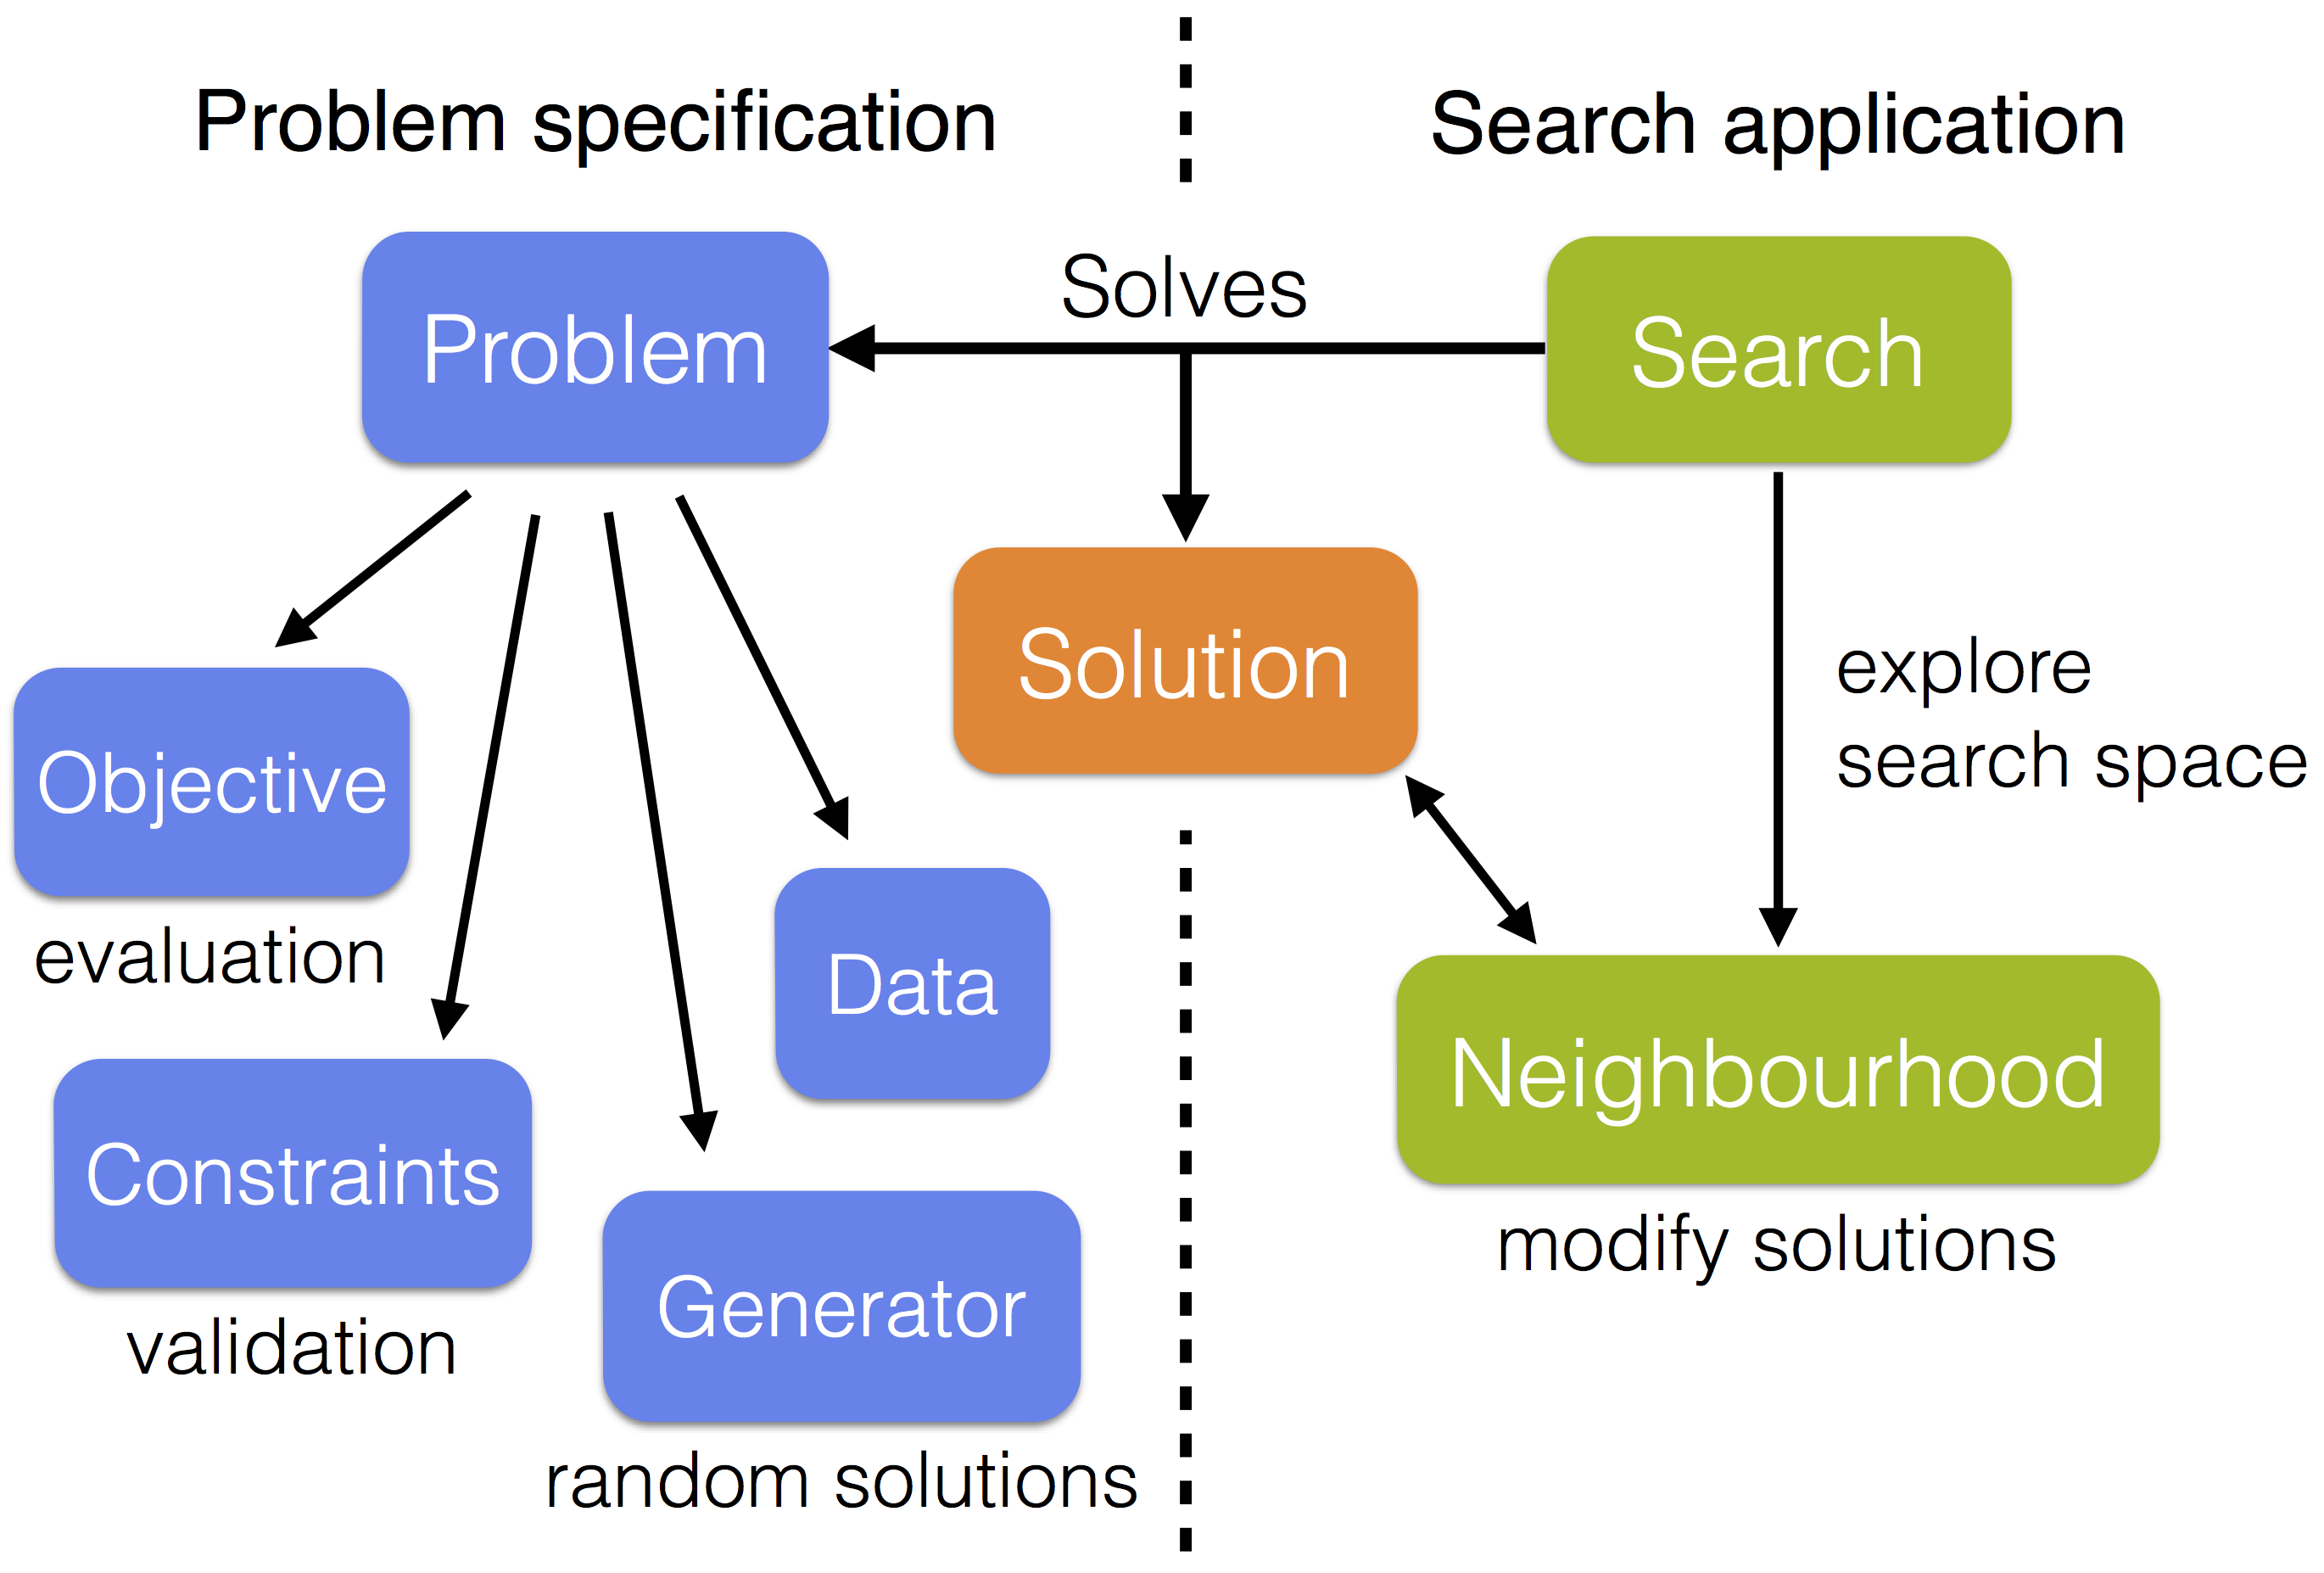
\includegraphics[scale=0.1]{images/diagram-detailed.png}
	\caption {
		 Diagram reprezentujący działanie biblioteki JAMES oraz elementy potrzebne do zdefiniowania problemu (źródło: \url{http://www.jamesframework.org/docs/})
	}
	\label{fig:james}
\end{figure}

Opis elementów biblioteki:
\begin{itemize}
    \item Solution - obiekt reprezentujący kompletne rozwiązanie problemu, który zawiera następujące dane
    \item Problem specification - specyfikacja problemu, która składa się z następujących elementów:
    \begin{itemize}
        \item Generator - obiekt służący do losowego generowania rozwiązań,
        \item Constraints - obiekty służace do walidacji rozwiązań pod względem spełniania stawianych warunków,
        \item Objective - obiekt służący do ewaluacji rozwiązania,
        \item Data - obiekt dostarczający przestrzeń rozwiązań.
    \end{itemize}
    \item Search application - zawiera następujące elementy:
    \begin{itemize}
        \item Search - znajduje się tutaj implementacja wybranego algorymu lokalnego przeszukiwania,
        \item Neighbourhood - obiekt umożliwiający modyfikacje rozwiązań w czasie działania algorytmu. Modyfikacje polegają na zmianie poszczególnych części rozwiązania na "sąsiednie".
    \end{itemize}
\end{itemize}

Biblioteka JAMES udostępnia szereg implementacji algorytmów metaheurystycznych służacych do lokalnego przeszukiwania przestrzeni rozwiązań w celu optymalizacji zadanego problemu. Wejściem każdego z algorytmów jest definicja problemu oraz kryterium stopu, które może być zdefiniowane jako maksymalny czas działania algorytmu bądź jako maksymalną liczbę kroków. W pracy zostały użyte następujące algorytmy pochodzące z tej biblioteki: Random Search, Random Descent, Steepest Descent, Tabu Search, Metropolis Search, Parallel Tempering.

\section{Dane opisujące właściwości żeliwa ADI}
\subsection{Zbieranie danych}
Dane na temat produkcji żeliwa ADI nie występują w sieci w postaci zagregowanej. Jedynymi źródłami, gdzie można je zdobyć, są artykuły oraz prace naukowe, w których autorzy podejmowali się badań nowych stopów i parametrów ich obróbki cieplnej. Rezultatami tych badań są w większości tabele przedstawiające jak dane składy wytopów oraz ich obróbka cieplna wpływały na właściwości mechaniczne. Część z artykułów, które zawierają bardzo obszerny przekrój różnych stopów i parametrów obróbki, przedstawia dane tylko w postaci wykresów, co wprowadza trudności w agregowaniu danych w jednym miejscu.

Zostało ustalone, że do zbioru danych będą zbierane następujące informacje:
\begin{itemize}
    \item skład chemiczny wytopu (zawartość procentowa pierwiastków):
    \begin{itemize}
        \item węgiel (C),
        \item krzem (Si),
        \item mangan (Mn),
        \item magnez (Mg),
        \item miedź (Cu),
        \item nikiel (Ni),
        \item molibden (Mo),
        \item siarka (S),
        \item fosfor (P),
        \item wanad (V),
        \item chrom (Cr).
    \end{itemize}
    \item ekwiwalent węglowy (CE) - obliczony jako\cite{joshi2020}: $CE = \%C+0.33(\%Si+\%P)$,
    \item parametry obróbki termicznej:    
    \begin{itemize}        
        \item temperatura i czas austenityzacji (aust\_temp, aust\_czas),       
        \item temperatura i czas ausferytyzacji (ausf\_temp, ausf\_czas).  
    \end{itemize}
    \item właściwości mechaniczne:    \begin{itemize}
        \item wytrzymałość na rozciąganie (Rm),
        \item granica plastyczności (Rp02),
        \item wydłużenie (A5),
        \item twardość,
        \item udarność.
    \end{itemize}
    \item grubość wytopu (mm),
    \item właściwości mechaniczne wytopu przed obróbką cieplną.
\end{itemize}

Budowa zbioru danych, który pozwoli na zbudowanie modeli predykcyjnych żeliwa ADI, okazała się procesem czasochłonnym. By lepiej zobrazować ten proces, zostały opracowane statystyki opisujące liczbę przeanalizowanych artykułów, zebranych rekordów, oraz rekordów odrzuconych na podstawie negatywnej oceny specjalistów.

Statystyki:
\begin{itemize}
    \item liczba zebranych artykułów/prac naukowych: 66,
    \item liczba zebranych rekordów (bez podziału na właściwości mechaniczne): 941 (w tym 252 rekordy odrzucone),
    \item liczba kompletnych rekordów (zawierających wszystkie właściwości mechaniczne, bez odrzuconych): 137,
    \item liczba zebranych rekordów (bez odrzuconych i z podziałem na właściwości mechaniczne): 1981,
    \item liczba unikalnych stopów: 94,
    \item liczba brakujących wartości: 1464 (42\% wszystkich możliwych wartości właściwości mechanicznych w zbiorze danych). 
\end{itemize}

Statystyka zebranych rekordów z podziałem na właściwości mechaniczne została przedstawiona na rysunku \ref{fig:stats}. Widać na nim, że dla dwóch właściwości mechanicznych (granica plastycznosci i udarność) liczbę zebranych danych w stosunku do wszystkich rekordów jest mniejsza niż 50\%. Dane te były najrzadziej występującymi w znalezionych pracach. Najczęściej występującymi danymi okazała się twardość, która była przestawiana w różnych skalach tj. skali twardości Brinella, skali twardości Rockwella oraz skali twardości Vickersa. Ze względu na większościowy udział danych przedstawionych w~postaci skali Brinella, dane w innych skalach zostały przekonwertowane do tej właśnie skali. Konwersja została przeprowadzona przy pomocy tabeli konwersji twardości \cite{hard_conversion}. Dodatkowym problemem okazała się udarność, gdyż także jest przedstawiana za pomocą dwóch różnych oznaczeń:
\begin{itemize}
    \item K - udarność mierzona na próbkach bez karbu,
    \item KV - udarność mierzona na próbkach z karbem V.
\end{itemize}
Ze względu na brak informacji o tym w jaki sposób te dwie wartości są ze sobą powiązane (brak danych opisujących jednocześnie udarność dla próbek z karbem oraz bez karbu), zostało założone, że $K = 11\cdot KV$ na podstawie tabel zawartych w normie PN-EN 1564:2012. Ze względu na większy udział rekordów zawierających udarność dla próbek bez karbu, rekordy z udarnością mierzoną na próbkach z karbem zostały przekonwertowane do wartości dla próbek bez karbu za pomocą wspomnianego wzoru.

\begin{figure}[ht]{}
	\centering
	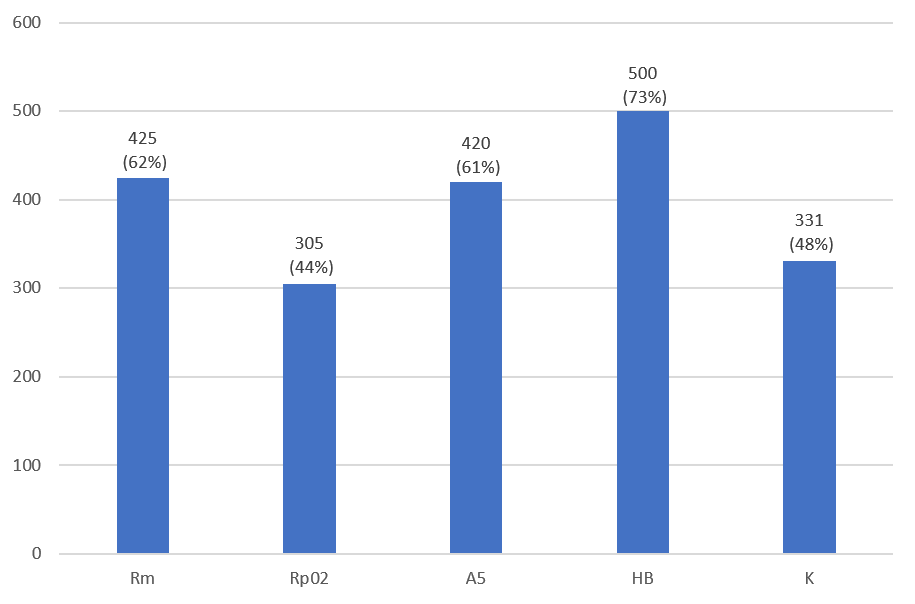
\includegraphics[scale=0.5]{images/statystyki.png}
	\caption {
		 Rozkład liczby zebranych danych dla każdej z właściwości mechanicznych.
	}
	\label{fig:stats}
\end{figure}

\subsection{Analiza zbioru danych}

W celu lepszego zrozumienia danych zostały sporządzone następujące graficzne reprezentacje:
\begin{itemize}
    \item wykresy pudełkowe - pozwalają na wskazanie wartości odstających,
    \item histogramy - pozwalają na wskazanie miejsc z brakującymi danymi,
    \item macierz korelacji - pozwala na określenie zależności między wymiarami.
\end{itemize}

Wykresy pudełkowe zostały sporządzone dla każdego z wymiarów i przedstawione w zagregowanej postaci na rysunkach \ref{fig:chem_box}, \ref{fig:heat_box} i \ref{fig:prop_thickness_box}. W przypadku wykresów dla składu chemicznego, w każdym wymiarze poza miedzią i niklem, wystepują wartości odstające. W~większości przypadków są to nieduże odstępstwa od średniej wartości w~danym wymiarze, więc można uznać, że są to mało pokryte zakresy wartości. Można jednak zauważyć wymiary, w których te odstępstwa są bardzo duże, co może wskazywać na błędy w~ artykułach, z których dane zostały zaczerpnięte. Przykładem może tutaj posłużyć wykres dla wymiaru fosforu, którego wartość średnia jest równa ok. 0,034, a największa wartość to 0,65, czyli 20 krotnie większa. Niestety, te odstępstwa nie zostały przeanalizowane przez ekspertów i przyjęte w badaniach jako poprawne. Dodatkową wadą wyrzucania wartości odstających w przypadku składu chemicznego byłoby wyrzucanie znacznej liczby rekordów ze zbioru, gdyż na każdy wytop przypada średnio ponad 9 rekordów.
\begin{figure}[ht]{}
	\centering
	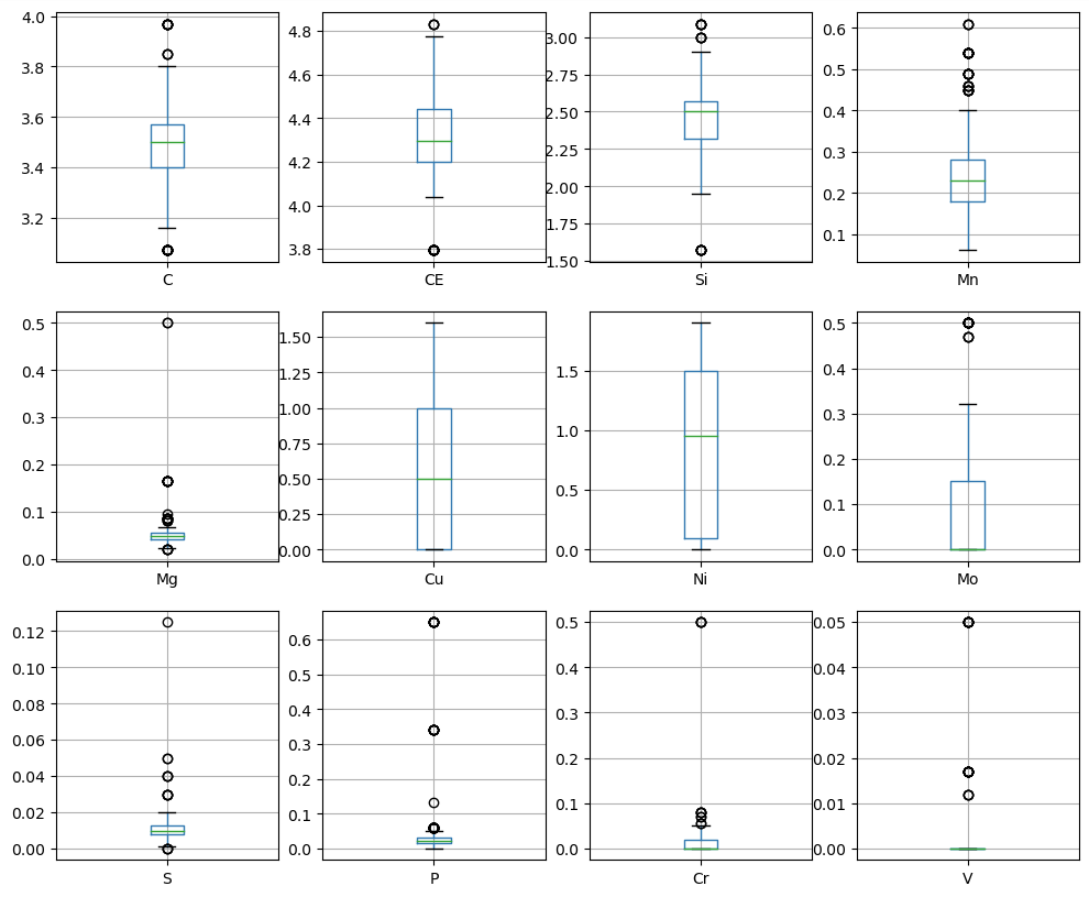
\includegraphics[scale=0.5]{images/chem_box.png}
	\caption {
		 Wykresy pudełkowe dla wymiarów składu chemicznego i ekwiwalentu węglowego.
	}
	\label{fig:chem_box}
\end{figure}

W przypadku wykresów dla wymiarów opisujących obróbkę termiczną, wymiarem rzucającym się w oczy jest temperatura austenityzacji. Wartość tego wymiaru oscyluje w okolicach wartości 900 stopni Celcjusza, gdyż jest to standardowa temperatura dla procesu austenityzacji. Wartości ukazane jako odstające, zostały celowo zostawione w zbiorze danych w celu zbadania jak inne wartości tej temperatury wpłyną na właściwości mechaniczne. Podobna sytuacja zachodzi w wymiarze opisującym temperaturę ausferrytyzacji - można zauważyć 3 wartości znacznie odstające od pozostałych danych lecz one także zostały zachowane w zbiorze danych.

\begin{figure}[ht]{}
	\centering
	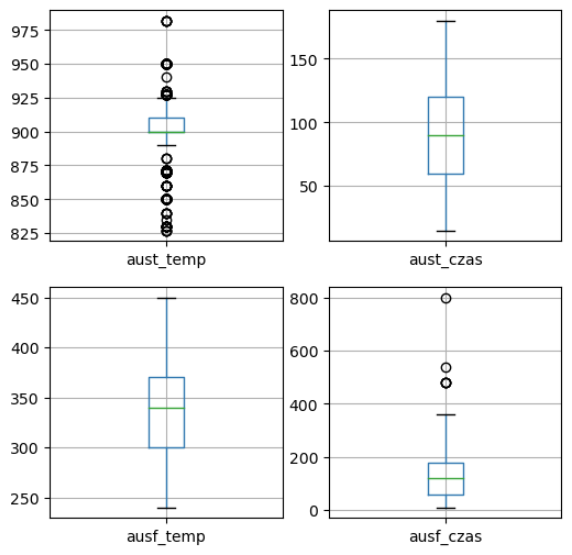
\includegraphics[scale=0.5]{images/heat_box.png}
	\caption {
		 Wykresy pudełkowe dla wymiarów obróbki termicznej.
	}
	\label{fig:heat_box}
\end{figure}

W przypadku wykresów dla właściwości mechanicznych oraz grubości, znacznie odstające dane można zauważyć w wymiarach K (udarność) oraz wymiarze opisującym grubość wytopu. Wartości odstające dla wymiaru udarności zostały pobrane z jednej pracy, która w sposób dokładny przedstawiła dane i nic nie wskazuje na to, by mogły być one niepoprawne. Dla wymiaru grubości wartości odstające wynikają z tego, że w większości prac badane były wytopy o grubości 25 mm.
\begin{figure}[ht]{}
	\centering
	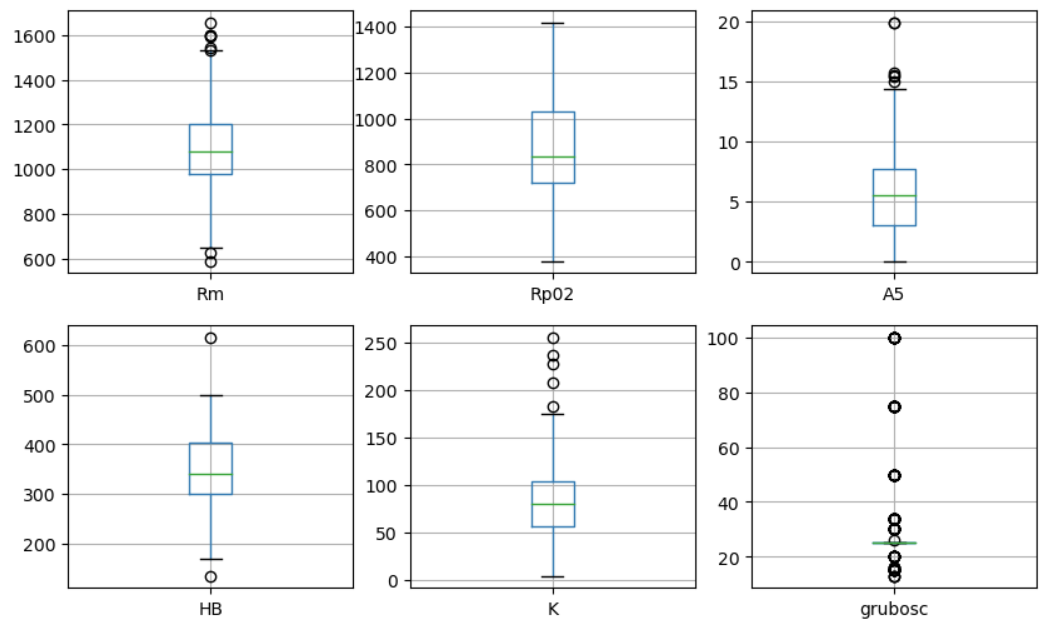
\includegraphics[scale=0.5]{images/prop_thickness_box.png}
	\caption {
		 Wykresy pudełkowe dla wymiarów właściwości mechanicznych oraz grubości wytopu.
	}
	\label{fig:prop_thickness_box}
\end{figure}

Histogramy zostały przedstawione na rys. \ref{fig:histogram}. Niektóre z nich są mało czytelne ze względu na znacznie odstające wartości. W przypadku wymiarów opisujących właściwości mechaniczne, histogramy pokazują, że rozkład każdego z nich ma kształt zbliżony do dzwonu oraz że w większości nie występują zakresy z brakującymi wartościami.
\begin{figure}[ht]{}
	\centering
	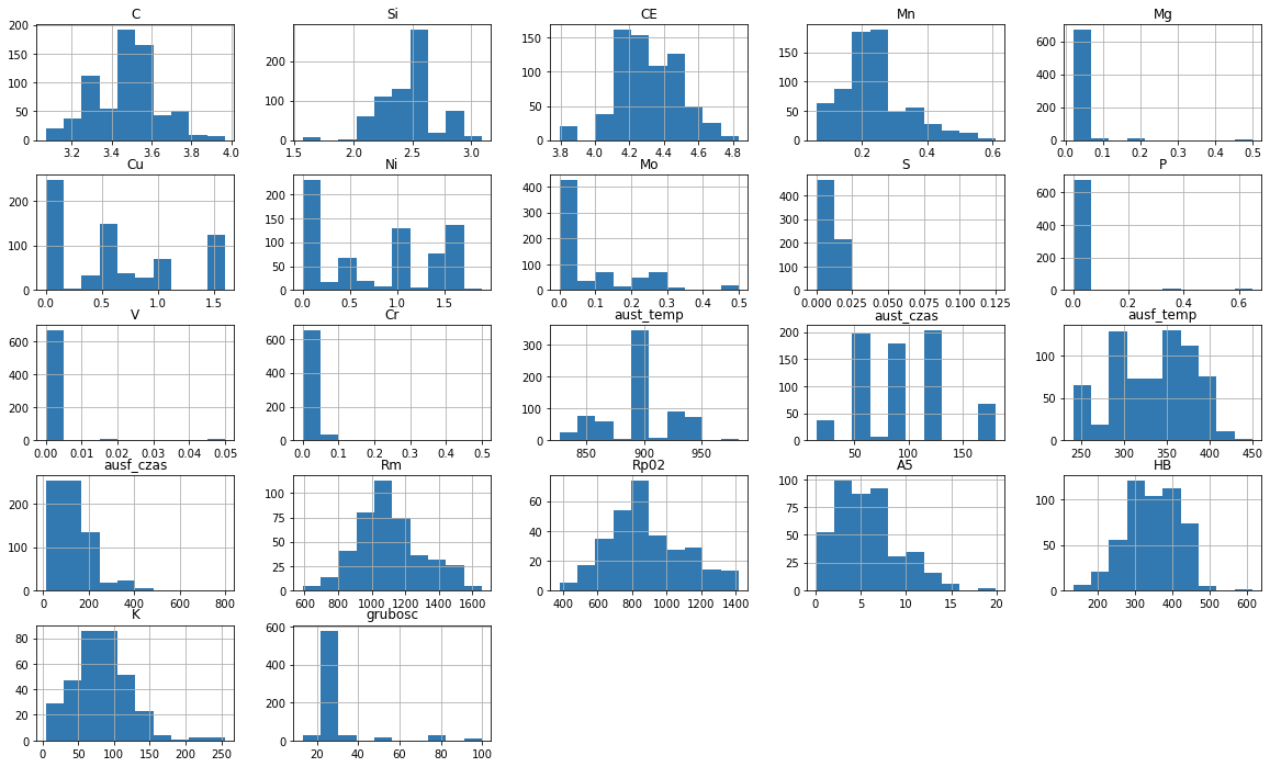
\includegraphics[scale=0.43]{images/histogram.png}
	\caption {
		 Histogramy dla wszystkich wymiarów w zbiorze danych.
	}
	\label{fig:histogram}
\end{figure}
\FloatBarrier
\subsection{Analiza korelacji zachodzących w zbiorze danych}\label{correlation-analysis}
\subsubsection{Macierz korelacji}
Macierz korelacji (rys. \ref{fig:correlation}) nie została przedstawiona dla wszystkich wymiarów ze względu na ich dużą liczbę oraz chęć zbadania korelacji między wymiarami opisującymi zależności miedzy procese produkcji i właściwościami mechanicznymi a właściwościami mechanicznymi. Widoczne w macierzy wartości są wartościami bezwględnymi w celu dostrzeżenia wymiarów najbardziej ze sobą skorelowanych. Macierz zostanie wykorzystana do analizy korelacji w zbiorze danych opisanej w punkcie \ref{correlation-analysis}.
\begin{figure}[ht]{}
	\centering
	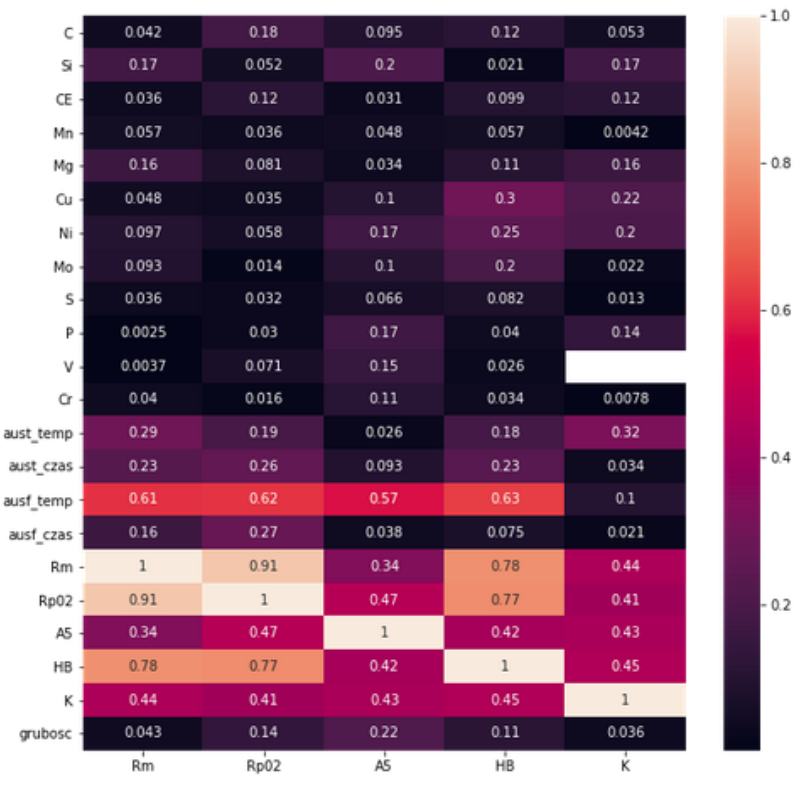
\includegraphics[scale=0.6]{images/correlation.png}
	\caption {
		 Macierz korelacji wszystkich wymiarów do wymiarów opisujących właściwości mechaniczne.
	}
	\label{fig:correlation}
\end{figure}
\FloatBarrier

\subsubsection{Analiza macierzy korelacji}
Przeprowadzona analiza powinna wskazać możliwość uzupełnienia brakujących danych wykorzystując inne wymiary, dla których wartości istnieją. 

Analizując macierz korelacji z rysunku \ref{fig:correlation}, można wyciągnąć następujące wnioski:
\begin{itemize}
    \item Zachodzi silna korelacja między wymiarami Rm oraz Rp02 (0.91),
    \item Wymiary Rm i Rp02 są także w znacznym stopniu skorelowane z wymiarem HB (0.78 i 0.77),
    \item Wymiar opisujący temperaturę ausferrytyzacji jest w pewnym stopniu skorelowany z wymiarami Rm, Rp02, A5, HB (ok. 0.6),
    \item Wymiar K opisujący udarność wygląda na słabo skorelowany z innymi wymiarami opisującymi właściwości fizyczne.
\end{itemize}

\subsubsection{Interpretacja wniosków do analizy korelacji}
Wnioski wyciągnięte podczas analizy korelacji pokazują w jasny sposób, że wymiary Rm, Rp02, A5, HB, ausf\_temp są ze sobą w znaczny sposób skorelowane i można założyć, że istnieje możliwość uzupełnienia brakujących danych w tych wymiarach wykorzystując inne istniejące już dane.
Ze względu na niski stopień korelacji wymiaru K do innych wymiarów, zostanie on pominięty na okres uzupełniania wyżej wymienionych wymiarów.

\subsection{Próba uzupełnienia brakujących danych}\label{sec:filling_data}

\subsubsection{Uproszczony sposób postępowania w celu uzupełnienia brakujących danych}
Problem brakujących danych został przedstawiony w pracy A. Kochańskiego pt. Knowledge in Imperfect Data \cite{Kochanski12}, gdzie zostało zaprezentowane przykładowe rozwiązanie. Mianowicie, w celu wypełnienia brakujących wartości należy znaleźć podzbiór próbek, w~ których dla wymiaru, w którym brakuje danych, istnieje wysoce skorelowany inny wymiar, na podstawie którego możliwe jest wyznaczenie brakującej wartości np. za pomocą regresji liniowej. W pracy stwierdzono, że zaletą takiego podejścia jest możliwość uzyskania nowych wartości granicznych zbioru danych. W przypadku, gdy korelacja między atrybutami nie występuje, brakująca wartość może zostać obliczona poprzez porównanie z~wybranymi rekordami ze zbioru zawierającego pełne dane.

\subsubsection{Przedstawienie metody uzupełniania brakujących danych}
Analizując przedstawiony powyżej uproszczony sposób postępowania w celu uzupełnienia brakujących danych, można wyciągnąć następujące założenia co do metody uzupełniania:
\begin{itemize}
    \item rozmiar podzbioru próbek powinien być określony, np. 10 próbek,
    \item może istnieć więcej niż jeden skorelowany wymiar, liczba takich wymiarów, która będzie brana pod uwagę powinna być określona, np. 2 wymiary,
    \item ze względu na duży rozrzut danych w zbiorze, podzbiór próbek powinien być wybrany w taki sposób, aby dane w wymiarach nieskorelowanych oraz niezwiązanych z właściwościami mechanicznymi żeliwa były dla siebie najbliższymi sąsiadami, 
    \item stosowanie regresji liniowej będzie adekwatne dla podzbiorów z bardzo wysokim współczynnikiem korelacji, tj. powyżej 0.8, dla podzbiorów z mniejszym współczynnikiem powinna zostać użyta inna metoda wyznaczania wartości (np. drzewa decyzyjne),
    \item im wyższy będzie współczynnik korelacji w danym podzbiorze oraz próbki z podzbioru będą w jak najmniejszej odległości od próbki, dla której będzie uzupełniana brakująca wartość, tym będzie bardziej prawdopodobne, że wyznaczona wartość będzie prawidłowa.
\end{itemize}

Dodatkowe założenia dotyczące metody uzupełniania:
\begin{itemize}
    \item ze względu na różną liczbę brakujących danych oraz różne stopnie skorelowania między wymiarami, w których istnieją brakujące dane, należy określić w jakiej kolejności wymiary będą uzupełnianie (np. na 3 pierwszych miejscach powinny się znajdować najliczniejsze wymiary, które są ze sobą mocno skorelowane - Rm, HB, Rp02),
    \item zakłada się, że uzupełnianie brakujących wartości może być realizowane z wykorzystaniem próbek, dla których wartości zostały uzupełnione we wcześniejszych etapach uzupełniania,
    \item korzystnym będzie uzupełnianie najpierw próbek, dla których w znalezionych podzbiorach jest wyższy współczynnik korelacji niż w pozostałych - w tym celu zakłada się, że na danym etapie uzupełniania danych będą uzupełniane tylko te próbki, dla których współczynnik korelacji dla podzbioru będzie wyższy lub równy progu, który będzie obowiązywał na danym etapie uzupełniania,
    \item ze względu na możliwość wykorzystania uzupełnionych danych przy uzupełnianiu innych, zakłada się, że proces uzupełniania dla konkretnego progu współczynnika korelacji będzie prowadzony dopóki istnieją próbki z podzbiorami spełniającymi dany próg (takie podejście pozwoli na wykorzystywanie próbek uzupełnionych w poprzednich krokach, które będą spełniały dany próg),
    \item ze względu na oczekiwane różne współczynniki korelacji w podzbiorach, zakłada się, że najpierw będą uzupełniane próbki z wysokimi współczynnikami korelacji wśród podzbiorów a następnie z mniejszymi,
    \item ze względu na to, że dla części danych znalezione podzbiory mogą mieć bardzo małe wartości korelacji, zakłada się ustalenie maksymalnej liczby etapów uzupełniania danych, po której proces uzupełniania zostanie przerwany.
\end{itemize}

Na podstawie powyższych założeń została sporządzona metoda uzupełniania brakujących wartości w zbiorze danych opisującym właściwości mechaniczne żeliwa ADI. 

W celu uzupełnienia brakujących danych należy ustalić:
\begin{itemize}
    \item kolejność uzupełnianych wymiarów,
    \item początkowy próg współczynnika korelacji (wspomniany w założeniach),
    \item liczba próbek w podzbiorze,
    \item granica współczynnika korelacji, do której stosowana będzie regresja liniowa,
    \item liczba wymiarów, na podstawie której przewidywana będzie brakująca wartość,
    \item algorytm uczenia maszynowego używany poza regresją liniową.
\end{itemize}

Metoda uzupełniania polega na znajdowaniu podzbioru próbek, które są najbliższymi sąsiadami uzupełnianej próbki dla wymiarów określonych jako nieskorelowane i nie będące związane z właściwościami fizycznymi żeliwa. Ustalanie brakującej wartości  polega na przewidywaniu jej wykorzystując model zbudowany z danych w znalezionym podzbiorze. W pierwszej kolejności uzupełniane są próbki, dla których średni współczynnik korelacji w~ ustalonym podzbiorze będzie przekraczał zadany próg. Próg wraz z brakiem zmiany liczby brakujących wartości, jest zmniejszany o ustaloną wartość np. 0.05. Próbki do ustalonej wartości współczynnika korelacji  w podzbiorze (np. 0.8) są uzupełniane za pomocą regresji liniowej, następnie wykorzystywany jest inny algorytm uczenia maszynowego np. drzewo decyzyjne. Dla danego progu współczynnika korelacji odbywa się pewna liczba kroków uzupełnienia brakujących wartości za sprawą wykorzystywania danych, które zostały uzupełnione we wcześniejszych krokach. Obniżenie progu następuje, gdy liczba brakujących danych się nie zmniejsza. Koniec uzupełniania następuje, gdy wszystkie brakujące wartości zostaną uzupełnione albo gdy liczba kroków przekroczy ustaloną maksymalną liczbę kroków.

\subsubsection{Pseudokod algorytmu}\label{sec:filling-pseudocode}
Pseudokod algorytmu został przedstawiony w trzech częściach, z których pierwsza (Algorytm \ref{algo:uzupelnianie}) przedstawia główne kroki algorytmu. 
Opis danych wejściowych alg. \ref{algo:uzupelnianie}:
\begin{itemize}
\item X - zbiór danych,
\item order - kolejność uzupełnianych wymiarów,
\item corr\_cutoff\_bound - początkowy próg korelacji,
\item req\_neighs - liczba próbek w podzbiorze, 
\item linear\_reg\_to - granica współczynnika korelacji, do której stosowana będzie regresja liniowa,
\item amount\_of\_feats\_to\_predict - liczba wymiarów, na podstawie której przewidywana jest brakująca wartość,
\item max\_steps - maksymalna liczba kroków,
\item next\_predictor\_provider - obiekt służący do zwracania algorytmu uczenia maszynowego używanego po przekroczeniu granicy używania regresji liniowej.
\end{itemize}
Wynik: zbiór danych uzupełniony w wymiarach określonych przez daną order.


Opis użytych funkcji pomocniczych i bardziej złożonych linii kodu w algorytmie \ref{algo:uzupelnianie}:
\begin{itemize}
    \item linia 2 - funkcja \textit{get\_missing\_values\_count}  przyjmująca zbiór próbek i zwracająca łączną liczbę brakujących wartości w wymiarach Rm, Rp02, HB, A5, K,
    \item linia 10 - wywołanie procedury \textit{fill\_missing} opisanej w algorytmie \ref{algo:fillMissing}
\end{itemize}

\begin{algorithm}[ht]
\DontPrintSemicolon
  \KwInput{order, corr\_cutoff\_bound, req\_neighs, linear\_reg\_to, amount\_of\_feats\_to\_predict, max\_steps, next\_predictor\_provider}
  \KwOutput{wypełniony zbiór próbek X}
  \SetKw{Continue}{continue}
  \KwData{zbiór próbek X}
  \SetKwFunction{getMissingValuesCount}{get\_missing\_values\_count}
  \SetKwFunction{getFeaturesWithNulls}{get\_features\_with\_nulls}
  \SetKwFunction{getCorrelationMatrix}{get\_correlation\_matrix}
  \SetKwFunction{mostCorrelatedFeaturesExceptNullFeatures}{most\_corr\_feats}
  \SetKwFunction{removeFeatsWithNulls}{remove\_features\_with\_nulls}
  \SetKwFunction{minMaxScaler}{min\_max\_scaler}
  \SetKwFunction{findNearestNeighs}{find\_nearest\_neighs}
  \SetKwFunction{fillMissing}{fill\_missing}
  \SetKwData{CorrCutoff}{corr\_cutoff}
  \SetKwData{MissingValuesCount}{missing\_values\_count}
  \SetKwData{Filled}{filled} 
  \SetKwData{NullFeatures}{null\_features} 
  \SetKwData{Correlated}{correlated} 
  \SetKwData{CorrelationMatrix}{corr\_matrix}
  \SetKwData{NotCorrelated}{not\_correlated}
  \SetKwData{Xprim}{X'}
  \SetKwData{Scaler}{scaler}
  \SetKwData{Neighs}{neighs}
  \SetKwData{NearestNeighs}{nearest\_neighbors}
  \SetKwData{Step}{step}
  \SetKwData{ActuallyMissing}{actually\_missing}

  $\CorrCutoff \leftarrow corr\_cutoff\_bound $\;
  $\MissingValuesCount \leftarrow \getMissingValuesCount(X) $\;
  \Repeat{\Filled == size(order) or step == max\_steps}{
    $\Filled \leftarrow 0 $\;
    \For{feature in order}{
        \If{all values for feature are filled}{
            $\Filled \leftarrow \Filled + 1 $\;
            \Continue
        }
        \For{row in X}{
            \tcp{procedura \fillMissing została zdefiniowana w algorytmie \ref{algo:fillMissing}}
            $\fillMissing(row, feature, amount\_of\_feats\_to\_predict, req\_neighs, \newline \hspace*{6em}corr\_cutoff, linear\_reg\_to, next\_predictor\_provider)$\;
        }
        $\Step \leftarrow \Step + 1$\;
        $\ActuallyMissing \leftarrow \getMissingValuesCount(X)$\;
        \If{\MissingValuesCount == \ActuallyMissing}{
            $corr\_cutoff \leftarrow corr\_cutoff - 0.05$\;
        }
        $\MissingValuesCount \leftarrow \ActuallyMissing $\;
    }
  }
  \KwRet{X}
  
    \caption{Uzupełnianie zbioru danych}\label{algo:uzupelnianie}
\end{algorithm}

\FloatBarrier

Opis danych wejściowych procedury \textit{fill\_missing} (alg. \ref{algo:fillMissing}):
\begin{itemize}
    \item row - wiersz ze zbioru próbek X, w którym będzie uzupełniana brakująca wartość,
    \item feature - nazwa aktualnie uzupełnianego wymiaru (np. Rm),
    \item amount\_of\_feats\_to\_predict - opisane dla alg. \ref{algo:uzupelnianie},
    \item req\_neighs - opisane dla alg. \ref{algo:uzupelnianie},
    \item corr\_cutoff - aktualny próg wartości współczynnika korelacji,
    \item linear\_reg\_to - opisane dla alg. \ref{algo:uzupelnianie},
    \item next\_predictor\_provider - opisane dla alg. \ref{algo:uzupelnianie}.
\end{itemize}

Opis użytych funkcji pomocniczych i bardziej złożonych linii kodu w algorytmie \ref{algo:fillMissing}:
\begin{itemize}
    \item linia 4 - funkcja \textit{get\_features\_with\_null} przyjmująca aktualnie rozpatrywany wiersz i zwracająca zbiór wszystkich wymiarów z tego wiersza, w których brakuje wartości,
    \item linia 7 - funkcja \textit{most\_corr\_feats} przyjmująca wartości współczynników korelacji do rozpatrywanego wymiaru (feature), stałą \textit{amounts\_of\_feats\_to\_predict} oraz zbiór wymiarów z brakującymi wartościami i zwracająca n najbardziej skorelowanych wymiarów do rozpatrywanego wymiaru (feature), gdzie n jest równe \textit{amounts\_of\_feats\_to\_predict},
    \item linia 11 - funkcja \textit{remove\_features\_with\_nulls} przyjmująca zbiór próbek X oraz zbiór wymiarów \textit{not\_correlated} i zwracająca zbiór wymiarów \textit{not\_correlated} z usuniętymi wymiarami, w których brakuje wartości,
    \item linia 13 i 14 - funkcja \textit{min\_max\_scaler} zwracająca obiekt skalera i przy wywołaniu funkcji \textit{scale} na tym obiekcie, zwraca zbiór próbek X' przeskalowany do wartości [-1, 1],
    \item linia 15 - nadpisanie składowej \textit{feature} wiersza ze zbioru próbek \textit{row} wartością zwróconą przez funkcję \textit{predict\_value}, która została przedstawiona w algorytmie \ref{algo:predictValue}.
\end{itemize}


\begin{algorithm}
    \caption{Procedura uzupełniania wartości brakującej w danej próbce}
    \label{algo:fillMissing}
    \DontPrintSemicolon
    
    \SetKw{Continue}{continue}
    \SetKwFunction{getMissingValuesCount}{get\_missing\_values\_count}
    \SetKwFunction{getFeaturesWithNulls}{get\_features\_with\_nulls}
    \SetKwFunction{getCorrelationMatrix}{get\_correlation\_matrix}
    \SetKwFunction{mostCorrelatedFeaturesExceptNullFeatures}{most\_corr\_feats}
    \SetKwFunction{removeFeatsWithNulls}{remove\_features\_with\_nulls}
    \SetKwFunction{minMaxScaler}{min\_max\_scaler}
    \SetKwFunction{findNearestNeighs}{find\_nearest\_neighs}
    \SetKwFunction{PredictValue}{predict\_value}
    \SetKwData{CorrCutoff}{corr\_cutoff}
    \SetKwData{MissingValuesCount}{missing\_values\_count}
    \SetKwData{Filled}{filled} 
    \SetKwData{NullFeatures}{null\_features} 
    \SetKwData{Correlated}{correlated} 
    \SetKwData{CorrelationMatrix}{corr\_matrix}
    \SetKwData{NotCorrelated}{not\_correlated}
    \SetKwData{Xprim}{X'}
    \SetKwData{Scaler}{scaler}
    \SetKwData{Neighs}{neighs}
    \SetKwData{NearestNeighs}{nearest\_neighbors}
    \SetKwProg{Proc}{Procedure}{ is}{end}
    \SetKwFunction{FillMissing}{fill\_missing}
    \Proc{\FillMissing{row, feature, amount\_of\_feats\_to\_predict, req\_neighs, corr\_cutoff, linear\_reg\_to, next\_predictor\_provider}}{
        \KwData{zbiór próbek X}
        \If{row[feature] is not null}{
                \Continue
            }
        $\NullFeatures \leftarrow \getFeaturesWithNulls(row) $\;
        $\NullFeatures.remove(feature) $\;
        $\CorrelationMatrix \leftarrow \getCorrelationMatrix(X) $\;
        $\Correlated \leftarrow \mostCorrelatedFeaturesExceptNullFeatures(\CorrelationMatrix[feature], \newline \hspace*{13em} amount\_of\_feats\_to\_predict, \newline
        \hspace*{13em} \NullFeatures)$\;
        $\Correlated.remove(feature)$\;
        $\NotCorrelated \leftarrow X.features - \Correlated$\;
        $\NotCorrelated.remove(feature)$\;
        $\NotCorrelated \leftarrow \removeFeatsWithNulls(X, \NotCorrelated)$\;
        $\Xprim \leftarrow X[\NotCorrelated]$\;
        $\Scaler \leftarrow \minMaxScaler(\Xprim)$\;
        $\Xprim \leftarrow \Scaler.scale(\Xprim)$\;
        \tcp{Funkcja \PredictValue została zdefiniowana w algorytmie \ref{algo:predictValue}}
        $row[feature] \leftarrow \PredictValue(\Xprim, \NotCorrelated, \Correlated, \Scaler, req\_neighs, \newline \hspace*{13em}amount\_of\_feats\_to\_predict, corr\_cutoff, \newline 
        \hspace*{13em}linear\_reg\_to, next\_predictor\_provider)$\;
    }
\end{algorithm}

\FloatBarrier
Opis danych wejściowych funkcji \textit{predict\_value} (alg. \ref{algo:predictValue}):
\begin{itemize}
    \item X' - zbiór przeskalowanych próbek zawierający wymiary nieskorelowane,
    \item not\_correlated - zbiór wymiarów nieskorelowanych,
    \item correlated - zbiór wymiarów skorelowanych,
    \item scaler - obiekt umożliwiający skalowanie wartości do zakresu [-1,1],
    \item req\_neighs - opisane dla alg. \ref{algo:uzupelnianie},
    \item amount\_of\_feats\_to\_predict - opisane dla alg. \ref{algo:uzupelnianie},
    \item corr\_cutoff - aktualny próg wartości współczynnika korelacji,
    \item next\_predictor\_provider - opisane dla alg. \ref{algo:uzupelnianie},
    \item linear\_reg\_to - opisane dla alg. \ref{algo:uzupelnianie}.
\end{itemize}

Opis użytych funkcji pomocniczych i bardziej złożonych linii kodu w algorytmie \ref{algo:predictValue}:
\begin{itemize}
    \item linia 4 - funkcja \textit{find\_nearest\_neighs} przymująca zbiór X', przeskalowany wektor wartości z wiersza\ textit{row} dla zbioru wymiarów \textit{not\_correlated} oraz liczba sąsiadów do znalezienia,
    \item linia 5 - funkcja \textit{remove\_neighs\_with\_nulls} przyjmująca zbiór najbliższych sąsiadów \textit{nns} i zbiór wymiarów skorelowanych \textit{correlated} i zwracająca tylko tych sąsiadów, dla których istnieją wartości we wszystkich skorelowanych wymiarach,
    \item linia 9 - funkcja \textit{features\_above\_corr\_cutoff} przyjmująca wektor współczynników korelacji dla wymiaru \textit{feature} pochodzący z macierzy korelacji \textit{corr\_matrix}, stałą \textit{amount\_of\_feats\_to\_predict} oraz stałą \textit{ corr\_cutoff} i zwracająca n najbardziej skorelowanych wymiarów, które spełniają warunek współczynnika korelacji większego lub równego \textit{corr\_cutoff} ( n - \textit{amount\_of\_feats\_to\_predict}).
\end{itemize}

\begin{algorithm}
    \DontPrintSemicolon
    
    \SetKw{Continue}{continue}
    \SetKwFunction{getMissingValuesCount}{get\_missing\_values\_count}
    \SetKwFunction{getFeaturesWithNulls}{get\_features\_with\_nulls}
    \SetKwFunction{getCorrelationMatrix}{get\_correlation\_matrix}
    \SetKwFunction{mostCorrelatedFeaturesExceptNullFeatures}{most\_corr\_feats}
    \SetKwFunction{removeFeatsWithNulls}{remove\_features\_with\_nulls}
    \SetKwFunction{minMaxScaler}{min\_max\_scaler}
    \SetKwFunction{findNearestNeighs}{find\_nearest\_neighs}
    \SetKwFunction{removeNeighsWithNulls}{remove\_neighs\_with\_nulls}
    \SetKwFunction{getFeatsAboveCorrCutoff}{features\_above\_corr\_cutoff}
    \SetKwData{CorrCutoff}{corr\_cutoff}
    \SetKwData{MissingValuesCount}{missing\_values\_count}
    \SetKwData{Filled}{filled} 
    \SetKwData{Predictor}{predictor} 
    \SetKwData{NullFeatures}{null\_features} 
    \SetKwData{Correlated}{correlated} 
    \SetKwData{CorrelationMatrix}{corr\_matrix}
    \SetKwData{NotCorrelated}{not\_correlated}
    \SetKwData{Xprim}{X'}
    \SetKwData{Neighs}{neighs}
    \SetKwData{NearestNeighs}{nns}
    \SetKwData{PredictedValue}{predicted\_value}
    \SetKwProg{Fn}{Function}{ is}{end}
    \SetKwFunction{PredictValue}{predict\_value}
    \Fn{\PredictValue{X’, not\_correlated, correlated, scaler, req\_neighs, amount\_of\_feats\_to\_predict, corr\_cutoff, linear\_reg\_to, next\_predictor\_provider}}{
        \KwResult{Przewidziana wartość}
        $\Neighs \leftarrow req\_neighs$\;
        \Repeat{size(\NearestNeighs) >= req\_neighs}{
            $\NearestNeighs \leftarrow \findNearestNeighs(\Xprim, scaler.scale(row[\NotCorrelated]), \Neighs)$\;
            $\NearestNeighs \leftarrow \removeNeighsWithNulls(\NearestNeighs, correlated)$\;
            $\Neighs \leftarrow \Neighs + (req\_neighs - size(\NearestNeighs))$\;
        }
        $\CorrelationMatrix \leftarrow \getCorrelationMatrix(\NearestNeighs) $\;
        $correlated \leftarrow \getFeatsAboveCorrCutoff(\CorrelationMatrix[feature], \newline \hspace*{13em}amount\_of\_feats\_to\_predict, corr\_cutoff)$\;
        \If{size(correlated) == 0}{
            \KwRet{null}
        }
        \If{corr\_cutoff >= linear\_reg\_to}{
            $\Predictor \leftarrow LinearRegression()$\;
        }
        \Else{
            $\Predictor \leftarrow next\_predictor\_provider.provide()$\;
        }
        $\Predictor.train(\NearestNeighs[correlated], \NearestNeighs[feature])$\;
        $\PredictedValue \leftarrow \Predictor.predict(row[correlated])$\;
        \If{\PredictedValue > 0}{\KwRet{\PredictedValue}}
        \Else{\KwRet{null}}
    }
    \caption{Funkcja przewidująca wartość służącą do uzupełniania próbki}
    \label{algo:predictValue}
\end{algorithm}

\FloatBarrier

\subsubsection{Implementacja algorytmu}
Algorytm został zaimplementowany przy użyciu narzędzi opisanych w sekcji \ref{sec:tools-data-analysis-modeling}. Implementacja opisanego algorytmu została wzbogacona o zbieranie informacji o~ sposobie uzupełniania brakujących danych:
\begin{itemize}
    \item wymiary służące do zbudowania podzbioru tzw. sąsiadów próbki,
    \item wymiary wybrane jako skorelowane w podzbiorze na podstawie których jest budowany model do przewidywania,
    \item współczynniki korelacji powyżej wspomnianych wymiarów do wymiaru, w którym była obecna brakująca wartość,
    \item wartość minimalna i maksymalna wymiaru z brakującą daną  w podzbiorze sąsiadów,
    \item indeksy próbek z podzbioru sąsiadów, które zostały wybrane do zbudowania modelu,
    \item numer kroku, w którym brakująca wartość została przewidziana.
\end{itemize}

\section{Budowa modeli predykcyjnych}\label{sec:model-realization}
Jak zostało już wspomniane w sekcji \ref{sec:model}, zachodzi potrzeba zbudowania modelu, który będzie reprezentował przestrzeń rozwiązań problemu opisanego w sekcji \ref{sec:problemDescription}. Nie było jednak możliwe zbudowanie wspólnego modelu dla wszystkich właściwości mechanicznych ze względu na podjęcię się tej części realizacji przed ukończeniem procesu uzupełniania danych, które nie przebiegło zgodnie z planem. 
Dla każdej z właściwości mechanicznych zostały zbudowane niezależne modele przy użyciu różnych zbiorów danych, które posiadały części wspólne ze względu na obecność rekordów o wszystkich właściwościach.

Do budowy takich modeli z powodzeniem stosowane są algorytmy uczenia maszynowego. W rozpatrywanym przypadku zostały wykorzystane modele regresyjne, które modelują związki pomiędzy dwiema lub więcej zmiennymi. Użyte algorytmy oraz narzędzia zostały opisane w sekcji \ref{sec:tools-data-analysis-modeling}.

\subsection{Redukcja wymiarowości zbioru, normalizacja i wymiar dogenerowany}
Ze względu na brak szczegółowej wiedzy na temat relacji między parametrami składu chemicznego a właściwościami mechanicznymi, przy redukcji wymiarowości została wzięta pod uwagę porada ekspertów. Zbiór danych został zredukowany o wymiary S, P, V, Cr ze względu na brak wpływu na właściwości mechaniczne oraz bardzo małą liczbę danych różnych od 0 w przypadku wymiarów Cr i V.

Wymiary wejściowe zostały znormalizowane metodą min-max do zakresu [-0.5;0.5]. Normalizacja została dokonana przy użyciu narzędzia MinMaxScaler z biblioteki scikit-learn. Warto tutaj wspomnieć, że normalizacja została dokonana na całym zbiorze danych przed podziałem na podzbiory dla właściwości mechanicznych.

Zbiór danych został rozszerzony o nowy wymiar, który przedstawia czas ausferrytyzacji przedstawiony w sekundach za pomocą logarytmu dziesiętnego. Takie rozszerzenie zbioru danych zostało zaproponowane w pracy M. A. Yescasa \cite{YESCAS2001162}, gdzie powołuje się on na swoją poprzednią pracę, w której dostrzegł, że taka forma lepiej opisuje czas ausferrytyzacji.

\subsection{Budowa zbioru treningowego i testowego}\label{sec:dataset}
Ze względu na małą liczbę próbek (689) w stosunku do liczby wymiarów (14) nie jest możliwe wyciągnięcie losowego zbioru próbek przeznaczonych na zbiór testowy bez utraty istotnych informacji ze zbioru treningowego. Aby temu zapobiec, została wykorzystana 5-krotna walidacja krzyżowa z zachowaniem takiego samego udziału próbek z każdej klasy. Ze względu na to, że wymiarami wyjściowymi są liczby, zostało stworzone 5 klas (1, 2, 3, 4, 5), które dzielą wartości na 5 zbiorów zbliżonych do siebie rozmiarem, poprzez ustalenie zakresu wartości wchodzących w skład danego zbioru. Liczność zbiorów reprezentujących klasy została przedstawiona na rys. \ref{fig:bins}. Zakresy wartości dla poszczególnych klas dla każdej z właściwości mechanicznych były następujące:
\begin{itemize}
    \item Rm: 1 - [Rm$_{min}$, 960), 2 - [960, 1045), 3 - [1045, 1127), 4 - [1127, 1264), 5 - [1264, Rm$_{max}$],
    \item Rp02: 1 - [Rp02$_{min}$, 696), 2 - [696, 813), 3 - [813, 900), 4 - [900, 1100), 5 - [1100, Rp02$_{max}$],
    \item HB : 1 - [HB$_{min}$, 286), 2 - [286, 325), 3 - [325, 370), 4 - [370, 415), 5 - [415, HB$_{max}$],
    \item A5 : 1 - [A5$_{min}$, 2.7), 2 - [2.7, 4.5), 3 - [4.5, 6.5), 4 - [6.5, 8.4), 5 - [8.4, A5],
    \item K : 1 - [K$_{min}$, 52), 2 - [52, 75), 3 - [75, 90), 4 - [90, 110), 5 - [110, K$_{max}$]
\end{itemize}

\begin{figure}[ht]{}
	\centering
	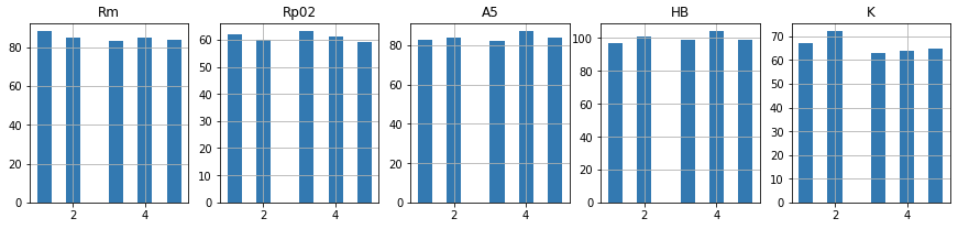
\includegraphics[scale=0.6]{images/bins.png}
	\caption {
		 Liczności zbiorów reprezentujących klasy, które rozdzielają wartości w wymiarach wyjściowych modeli.
	}
	\label{fig:bins}
\end{figure}
\FloatBarrier

\subsection{Trenowanie modeli}
Proces trenowania modeli został przeprowadzony w następujący sposób:
\begin{itemize}
    \item trenowanie każdego z modeli zostało przeprowadzone z wykorzystaniem walidacji krzyżowej wspomnianej w punkcie \ref{sec:dataset},
    \item dla każdego z algorytmów zostały wybrane różne wartości parametrów sterujących ich działaniem
    \item tuning parametrów został przeprowadzony poprzez trenowanie modeli dla każdej permutacji parametrów algorytmu,
    \item metryki użyte w celu oceny jakości wytrenowanych modeli: \begin{itemize}
        \item MAE (mean absolute error) - średni błąd bezwzględny,
        \item $R^{2}$ - współczynnik determinacji,
    \end{itemize}
    \item model po ewaluacji metryk jest douczany na zbiorze testowym,
    \item do badań porównawczych zostały wykorzystane po jednym najlepszym modelu dla każdej z metryk (sekcja \ref{sec:comp-eval}).
\end{itemize}

\subsubsection{Trenowanie modeli z wykorzystaniem algorytmu Random Forest} \label{sec:rf-train}
Algorytm Random Forest w przypadku implementacji pochodzącej z biblioteki scikit-learn posiada wiele parametrów, które wpływają na jego działanie. W celu znalezienia najlepszych modeli, zostały przetestowane następujące parametry:
\begin{itemize}
    \item n\_estimators - liczba drzew w lesie,
    \item max\_depth - maksymalna głębokość drzew,
    \item max\_features - liczba wymiarów rozpatrywanych przy szukaniu najlepszego podziału,
    \item criterion - metryka służąca do pomiaru jakości podziału,
    \item min\_samples\_split - minimalna liczba próbek potrzebna do podzielenia węzła w~ drzewie.
\end{itemize}
\subsubsection{Trenowanie modeli z wykorzystaniem algorytmu Gradient Boosting}\label{sec:gb-train}
Trenowanie modeli z użyciem algorytmu Gradient Boosting zostało przeprowadzone w identyczny sposób jak w przypadku trenowania modeli z użyciem algorytmu Random Forest.

Parametry algorytmu użyte podczas badań:
\begin{itemize}
    \item learning\_rate,
    \item subsample - współczynnik określający jaka część próbek treningowych zostanie losowo wybrana do trenowania przed rozrastaniem się drzew,
    \item max\_depth - maksymalna głębokość drzewa,
    \item eval\_metric - metryka służąca do ewaluacji modelu,
    \item booster - rodzaj używanego boostera.
\end{itemize}

Kombinacja wszystkich możliwych parametrów tworzy 216 unikalnych zbiorów. Podobnie jak w poprzednim algorytmie, parametr random\_state był ustawiony z jedną wartością dla każdego procesu uczenia.

W celu zbadania przestrzeni parametrów ponownie zostało zastosowane narzędzie GridSearchCV. Czas potrzebny na wytrenowanie wszystkich modeli wyniósł 10 sekund.

\subsubsection{Trenowanie modeli z wykorzystaniem algorytmu Multilayer Perceptron}\label{sec:mlp-train}
Do tworzenia i trenowania modeli z wykorzystaniem algorytmu Multilayer Perceptron został wykorzystany interfejs Keras z biblioteki TensorFlow. Pozwala on na czytelne i~proste definiowanie architektury sieci neuronowej poprzez tworzenie modelu sekwencyjnego, do którego dodajemy kolejne warstwy sieci. Taki model jest ostatecznie kompilowany z użyciem wskazanej metody stochastycznego spadku wzdłuż gradientu oraz funkcją straty.

Tworzone modele sieci neuronowych składają się z trzech warstw sieci:
\begin{itemize}
    \item warstwa wejściowa z 14 neuronami,
    \item warstwa ukryta, dla której zostały zbadane następujące parametry i ich wartości:
    \begin{itemize}
        \item funkcja aktywacji: tangens hiperboliczny,
        \item regularyzacja L2 dla wag, biasów oraz wyjścia warstwy,
    \end{itemize}
    \item warstwa wyjściowa z jednym neuronem.
\end{itemize}
Modele kompilowane są przy użyciu optymalizatora Adam z parametrem 'learning\_rate' ustawionym na wartość 0.1 oraz funkcją straty zdefiniowaną jako błąd średniokwadratowy.

Proces uczenia został przeprowadzony z użyciem metody Early Stopping, która pozwala zapobiegać przeuczeniu się sieci poprzez sprawdzanie, czy wartość funkcji straty dla próbek walidacyjnych zmienia się trakcie procesu uczenia. 

\subsubsection{Trenowanie modeli z wykorzystaniem algorytmu Ensemble averaging}\label{sec:ea-train}
Budowa modelu z wykorzystaniem tego algorytmu została zaczerpnięta z pracy Miguela Yescasa \cite{YESCAS2001162}, gdzie autor w swojej pracy nazwał go modelem komitetu sieci neuronowych. Więcej informacji na temat tej pracy znajduje się w sekcji \ref{sec:sota-prediction}.

Algorytm Ensemble averaging polega na stworzeniu wielu modeli o różnych parametrach i połączeniu ich w jeden model w taki sposób, by wejście i wyjście takiego modelu nie różniło się niczym od pojedyńczego modelu. Wyjście modeli jest połączone i ostateczne wyjście modelu jest średnią wartością wyjść modeli wchodzących w skład komitetu.

Modele wchodzące w skład komitetu sieci zostały wytrenowane z różnymi stałymi regularyzacji oraz różnymi liczbami neuronów wchodzących w skład warstwy ukrytej. By ograniczyć liczbę różnych stałych regularyzacji, zostało przeprowadzone badanie mające na celu sprawdzić, które stałe będą się najlepiej spisywać dla modeli z 10 oraz 25 neuronami w warstwie ukrytej. 

Zbadanymi stałymi dla wag, biasów oraz wyjść warstwy były wartości:  [1e-1, 1e-2, 1e-3, 1e-4, 1e-5]. Badanie zostało przeprowadzone z użyciem 5-krotnej walidacji krzyżowej wraz ze zbieraniem wartości metryk $R^{2}$ i średniego błędu absolutnego. Analiza badań opisana w punkcie \ref{sec:ea-eval} dostarczyła wartości stałych, które zostały przedstawione w tabeli \ref{tab:regularization}.
\begin{table}
\caption{Najlepsze stałe regularyzacji względem metryki $R^{2}$ dla sieci z 25 i 10 neuronami w warstwie ukrytej}
    \label{tab:regularization}
    \centering
    \begin{tabular}{|c|c|c|c|c|}
        \hline
        \multirow{2}{*}{Właściwość} & \multirow{2}{*}{Liczba neuronów} & \multicolumn{3}{|c|}{Stałe regularyzacji} \\
        \cline{3-5}
        && wagi & bias & wyjście \\
         \hline
        \multirow{4}{*}{Rm} & \multirow{2}{*}{25} & 1e-5 & 1e-4 &1e-1 \\
        \cline{3-5}
        && 1e-3 &1e-5 & 1e-5 \\
        \cline{2-5}
        & \multirow{2}{*}{10} & 1e-4 & 1e-5 & 1e-3 \\ 
        \cline{3-5}
        && 1e-2	& 1e-2 &1e-5 \\
        \hline
        \multirow{4}{*}{Rp02} & \multirow{2}{*}{25} & 1e-1 &1e-1 & 1e-5 \\
        \cline{3-5}
        && 1e-5 &1e-4 &1e-4 \\
        \cline{2-5}
        & \multirow{2}{*}{10} & 1e-2 & 1e-2 & 1e-2 \\ 
        \cline{3-5}
        && 1e-4 & 1e-3 & 1e-2 \\
        \hline
        \multirow{4}{*}{A5} & \multirow{2}{*}{25} & 1e-4 & 1e-3&1e-5 \\
        \cline{3-5}
        && 1e-3&1e-4&1e-5 \\
        \cline{2-5}
        & \multirow{2}{*}{10} & 1e-3&1e-1&1e-3 \\ 
        \cline{3-5}
        && 1e-3	& 1e-5&	1e-2 \\
        \hline
        \multirow{4}{*}{HB} & \multirow{2}{*}{25} & 1e-1&1e-3&1e-3 \\
        \cline{3-5}
        && 1e-1	&1e-2&1e-5 \\
        \cline{2-5}
        & \multirow{2}{*}{10} & 1e-3&1e-3&1e-2 \\ 
        \cline{3-5}
        && 1e-2&1e-4&1e-2 \\
         \hline
        \multirow{4}{*}{K} & \multirow{2}{*}{25} & 1e-1	&1e-5&1e-5 \\
        \cline{3-5}
        && 1e-1&1e-2&1e-3 \\
        \cline{2-5}
        & \multirow{2}{*}{10} & 1e-1&1e-2&	1e-1 \\ 
        \cline{3-5}
        && 1e-3&1e-2&1e-5 \\
        \hline
    \end{tabular}
    
\end{table}

Parametry, z jakimi były trenowane modele:
\begin{itemize}
    \item funkcja aktywacji: tangens hiperboliczny,
    \item stałe regularyzacji: określone w tabeli \ref{tab:regularization},
    \item liczba neuronów w wartwie ukrytej: [3...30],
    \item optymalizator: Adam z parametrem learning\_rate równym 0.01,
    \item optymalizowana funkcja: błąd średniokwadratowy,
    \item maksymalna liczba epok: 3000,
    \item rozmiar wsadu: 10,
    \item liczba epok bez zmian wartości funkcji straty, po których proces uczenia zostanie zakończony: 100.
\end{itemize}

Modele do budowy komitetów były wybierane na dwa sposoby:
\begin{itemize}
    \item Został stworzony ranking konfiguracji modeli, w którym o miejscu decydowała średnia wartość metryki $R^{2}$ lub średniego błędu bezwzględnego ze wszystkich podziałów zbioru danych pochodzących z walidacji krzyżowej. Dla każdego z podziałów zbioru był budowany model komitetu składający się z n najlepszych modeli według stworzonego rankingu i końcowa jakość modelu została obliczona jako średnia wartość metryk każdego z modeli komitetu z każdego podziału.
    \item Dla każdego z podziałów został stworzony model komitetu, gdzie w jego skład wchodziło n najlepszych modeli względem metryki $R^{2}$ lub średniego błędu bezwzględego dla danego podziału zbioru danych. Końcowa jakość modelu została obliczona jako średnia wartość metryk każdego z modeli komitetu z każdego podziału.
\end{itemize}

Pierwsza strategia będzie oznaczana jako 'avg' (od średniej wartości metryki) a druga jako 'split' (od podziału pochodzacego z walidacji krzyżowej).

Badaniu została poddana różna liczba modeli wchodzących w skład komitetu. Zbadany został zakres od 2 do 30 modeli dla każdej z właściwości mechanicznych.

\section{Realizacja optymalizacji heurystycznej}\label{sec:opt-realization}
Optymalizacja heurystyczna opisana w punkcie \ref{sec:heur-opt} została zrealizowana przy użyciu biblioteki JAMES dla języka programowania Java. Wspiera ona implementacje optymalizacji heurystycznej przy użyciu metaheurystycznych algorytmów lokalnego przeszukiwania. Opis biblioteki został przedstawiony w sekcji \ref{sec:james}. Poniższe podsekcje zawierają bardziej szczegółowy opis elementów stworzonych na potrzeby optymalizacji.

\subsection{Elementy potrzebne do przeprowadzenia optymalizacji}
\subsubsection{Dane}
Dane używane w czasie optymalizacji składają się z następujących części:
\begin{itemize}
    \item zbiór wszystkich możliwych wartości parametrów produkcji, które tworzą przestrzeń rozwiązań dla algorytmów przeszukujących, w której dostępne wartości są podzielone na następujące skończone zbiory:
    \begin{itemize}
        \item zbiór składów chemicznych wytopów, które znajdują się w zbiorze danych,
        \item zbiory wartości parametrów obróbki termicznej, w których wartości są elementami ciągów arytmetycznych (więcej informacji w punkcie \ref{sec:param_set}),
    \end{itemize}
    \item wytrenowane modele, które przewidują wartości mechaniczne dla zadanych parametrów produkcji.
\end{itemize}

\subsubsection{Ewaluacja rozwiązania}
Ewaluowanie rozwiązań w czasie działania algorytmów optymalizacji zostało zrealizowane przy użyciu funkcji QC opisanej w punkcie \ref{sec:opt}. Wagi kryteriów kosztu i jakości są dostarczane z systemu opisanego w punkcie \ref{sec:system}.

\subsubsection{Generator rozwiązań}
Generator rozwiązań ma za zadanie znaleźć losowe rozwiązanie dla problemu produkcji żeliwa ADI, które będzie spełniało wymagania narzucone przez normę. Wyszukiwanie losowego rozwiązania polega na wybieraniu losowych elementów wchodzących w skład rozwiązania:
\begin{itemize}
    \item losowo wybrany skład chemiczny wytopu, 
    \item losowo wybrane parametry obróbki termicznej.
\end{itemize}
Możliwe wartości dostarczane są wraz z danymi opisanymi punkcie 'Dane'.

\subsubsection{Modyfikacja rozwiązań}\label{sec:neighs}
Do poprawnego działania algorytmów lokalnego przeszukiwania należy zdefiniować tzw. sąsiedztwo, czyli rozwiązania, które są w sąsiedztwie rozpatrywanego rozwiązania. W~ przypadku biblioteki JAMES, takie sąsiedztwo jest osiągalne po zdefiniowaniu sposobu na modyfikację rozwiązania. W tym celu zostały zdefiniowane dwa sposoby modyfikacji rozwiązania:
\begin{itemize}
    \item zmiana losowego parametru obróbki termicznej, która polega na ustawieniu wartości sąsiedniej (losowo mniejszej lub większej),
    \item zmiana na inny losowy skład chemiczny wytopu.
\end{itemize}
Implementacje takich zmian muszą zawierać możliwość cofnięcia dokonanej zmiany.

\subsubsection{Definicja problemu}
Do poprawnego działania biblioteki JAMES należy zdefiniować problem, jaki będzie przekazany algorytmowi przeszukującemu w celu rozwiązania. Definicja problemu polega na stworzeniu obiektu generycznego problemu, który należy zaopatrzyć w następujące elementy:
\begin{itemize}
    \item dane - wspomniane powyżej w sekcji 'Dane',
    \item cel - obiekt dostarczający ewaluacje rozwiązań, zdefiniowany jako minimalizacyjny,
    \item generator losowych rozwiązań,
    \item ograniczenia - określające czy dane rozwiązanie spełnia wymagania stawiane przez normę.
\end{itemize}

\section{System wspomagania decyzji}\label{sec:system}
Koncepcja pracy zakłada stworzenie systemu wspomagania decyzji (opis w punkcie \ref{sec:dec-sup-sys-concept}) wykorzystującego elementy, których realizacja została opisana w punktach \ref{sec:model-realization} oraz \ref{sec:opt-realization}. Ze względu na liczbę danych, które należy wprowadzić do systemu oraz dodatkowe elementy, które nie zostały wymienione w koncepcji, podjęto decyzję, że interfejs systemu zostanie wykonany w postaci graficznego interfejsu użytkownika. Do jego wykonania został użyty język programowania Java w wersji 11 wraz z frameworkiem OpenJFX, który to pozwala na szybkie definiowane widoków oraz manipulowanie danymi wprowadzanymi przez użytkownika.

Stworzony system składa się z następujących elementów:
\begin{itemize}
    \item graficzny interfejs użytkownika,
    \item ładowanie modeli wytrenowanych z użyciem bibliotek Keras i XGBoost (w przypadku modeli wytrenowanych z użyciem biblioteki scikit-learn nie została znaleziona oficjalna biblioteka służąca do ich obsługi w technologii Java więc system ich nie wspiera),
    \item optymalizacja - instancjonowanie problemu oraz algorytmu przeszukującego oraz sterowanie i monitorowanie procesu optymalizacji.
\end{itemize}

W poniższych podsekcjach wyżej wymienione elementy zostały dokładniej przedstawione.

\subsection{Graficzny interfejs użytkownika}
Interfejs użytkownika został podzielony na następujące tematyczne zakładki:
\begin{itemize}
    \item Konfiguracja (rys. \ref{fig:conf}) - kontrolki służące do ustalenia następujących parametrów:
    \begin{itemize}
        \item stosunek kosztu do jakości,
        \item grubość stopu,
        \item wymagana norma.
    \end{itemize}
    \item Norma (rys. \ref{fig:norm}) - kontrolka służąca do zmiany zakresu grubości stopu oraz tabela służąca do podejrzenia i wprowadzenia zmian wartości w normie (domyślne wartości pochodzą z normy PN:EN 1564:2012) 
    \item Parametry funkcji kosztu (rys. \ref{fig:cost-tab}) - kontrolki służące do wprowadzania takich informacji jak:
    \begin{itemize}
        \item Średnia cena żeliwa,
        \item Średnia waga wsadu,
        \item Cena niklu,
        \item Cena miedzi,
        \item Cena molibdenu.
    \end{itemize}
    \item Zakresy produkcyjne (rys. \ref{fig:prod-range-tab}) - tabela służąca do edycji zakresów produkcyjnych wybranych parametrów oraz ich stopnia ważności przy wyznaczaniu jakości,
    \item Uruchamianie algorytmu (rys. \ref{fig:algo-run-tab}) - zestaw kontrolek służących do:
    \begin{itemize}
        \item generowania, usuwania, zapisu, przywracania oraz wprowadzania parametrów rozwiązania,
        \item wyświetlania aktualnych parametrów rozwiązania,
        \item wyświetlania ceny, jakości oraz wartości właściwości mechanicznych aktualnego rozwiązania,
        \item wyboru algorytmu i określenia maksymalnego czasu działania,
        \item uruchamiania i zatrzymywania algorytmów,
        \item wyświetlania postępów działania algorytmu.
    \end{itemize}
\end{itemize}
\begin{figure}
    \begin{subfigure}[b]{0.3\textwidth}
        \centering
        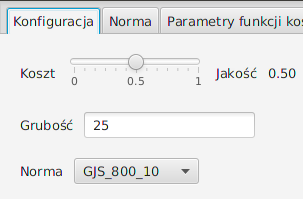
\includegraphics[scale=0.6]{images/conf.png}
        \caption {
            Konfiguracja
        }
        \label{fig:conf}
    \end{subfigure}
   \hfill
    \begin{subfigure}[b]{0.7\textwidth}
    	\centering
    	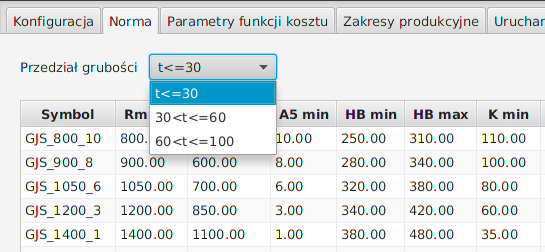
\includegraphics[scale=0.6]{images/norm.png}
    	\caption {
    		 Norma
    	}
    	\label{fig:norm}
    \end{subfigure}
    \vfill
    \begin{subfigure}[b]{0.3\textwidth}
    	\centering
    	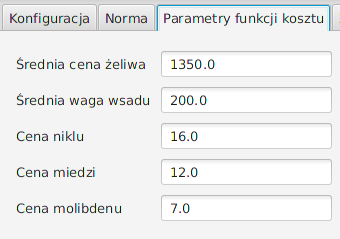
\includegraphics[scale=0.6]{images/cost.png}
    	\caption {
    		 Parametry funkcji kosztu
    	}
	    \label{fig:cost-tab}
    \end{subfigure}
    \hfill
    \begin{subfigure}[b]{0.7\textwidth}
    	\centering
    	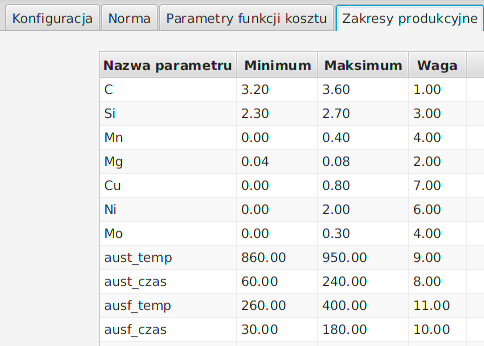
\includegraphics[scale=0.6]{images/prod_range.png}
    	\caption {
    		 Zakresy produkcyjne
    	}
    	\label{fig:prod-range-tab}
    \end{subfigure}
    \vfill
    \begin{subfigure}[b]{\textwidth}
    	\centering
    	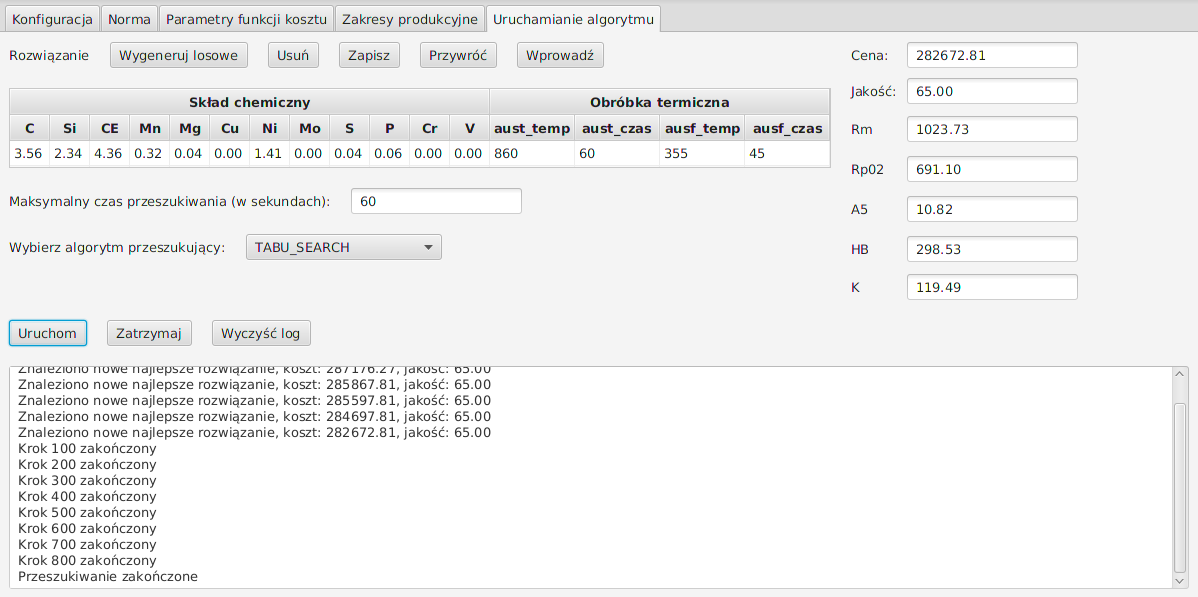
\includegraphics[scale=0.45]{images/algo_run.png}
    	\caption {
    		 Uruchamianie algorytmu
    	}
    	\label{fig:algo-run-tab}
    \end{subfigure}
    \caption{Zrzuty ekranu z graficznego interfejsu użytkownika}
    \label{fig:three graphs}
\end{figure}

Sposób uruchomienia i dodatkowe opisy zostały zawarte w załączniku na końcu pracy.

\FloatBarrier

\subsection{Ładowanie i używanie modeli w systemie}
Proces ładowania modeli odbywa się podczas ładowania systemu. Cała konfiguracja do tego służąca została zdefiniowana w postaci pliku o formacie JSON, w którym znajdują się ścieżki do modeli i ich konfiguracje warst wejściowych wraz z wartościami minimalnymi i maksymalnymi oraz przesunięciem, które służą do normalizacji wartości wejściowych modeli. Dodatkowo, w pliku konfiguracji znajduje się ścieżka do pliku w formacie JSON zawierającego wszystkie możliwe wartości, z których budowana jest przestrzeń rozwiązań dla algorytmów przeszukiwania. 

System obsługuje dwa źródła modeli:
\begin{itemize}
    \item modele wytrenowane za pomocą biblioteki XGBoost
    \item modele wytrenowane za pomocą biblioteki Keras
\end{itemize}

W pliku konfiguracyjnym należy podać typ modelu, czyli bibliotekę w której został wytrenowany. Przykładowa definicja modelu twardości została przedstawiona na rys. \ref{fig:hb-xgb}.

\begin{figure}[ht]{}
	\centering
	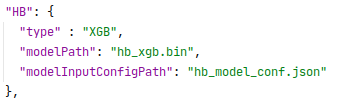
\includegraphics[scale=0.8]{images/hb-xgb.png}
	\caption {
		 Fragment konfiguracji systemu przedstawiający przykładową konfigurację modelu twardości.
	}
	\label{fig:hb-xgb}
\end{figure}








\chapter{Ewaluacja} \label{chap:evaluation}
Ten rozdział został poświęcony przedstawieniu badań nad elementami poruszonymi w poprzednim rozdziale. W sekcji \ref{sec:filling-research} zostały opisane zmagania związane z przetestowaniem parametrów algorytmu uzupełniania danych opisanego w sekcji \ref{sec:filling_data}. Badania nad algorytmem zostały przeprowadzone dwuetapowo, gdzie w pierwszym etapie zostało wyłonione 16 najlepszych konfiguracji parametrów, które w drugim etapie zostały ponownie przetestowane z większą liczbą kroków algorytmu.

Sekcja \ref{sec:models-eval} została poświęcona szczegółowemu przetestowaniu wybranych algorytmów uczenia maszynowego (sekcja \ref{sec:model}). Każdy z algorytmów został sprawdzony pod kątem jakości dla dwóch znanych metryk: średniego błędu bezwzględnego (MAE) oraz współczynnika determinacji $R^{2}$. Najlepsze konfiguracje dla każdego z algorytmu zostały następnie ze sobą porównane i został wytypowany algorytm, który cechuje się najlepszą jakością przewidywania dla stworzonego zbioru danych z sekcji \ref{sec:dataset}.

W ostatniej sekcji (\ref{sec:opt-research}) opisane zostały badania algorytmów optymalizacji wybranych w sekcji \ref{sec:algos}. Na wstępie został przeprowadzony test determinizmu, którego celem było sprawdzenie, czy jak algorytmy radzą sobie z optymalizacją dla różnych ziaren losowości. Dalsze testy zostały przeprowadzone dla dwóch różnych rozwiązań początkowych oraz 3 konfiguracji wag kryteriów kosztu i jakości. Ostatecznie zostały wybrane dwa różne algorytmy, które osiągnęły najlepsze wyniki.

\section{Badanie algorytmu uzupełniania danych}\label{sec:filling-research}
W tej sekcji zostały opisane badania algorytmu przedstawionego w sekcji \ref{sec:filling_data}, których celem jest znalezienie jakie wartości parametrów pozwolą na poprawne uzupełnienie danych w stworzonym zbiorze danych. 

\subsection{Badane parametry algorytmu}
Badania zostały przeprowadzone na parametrach z następującymi wartościami (parametry zostały opisane w sekcji \ref{sec:filling-pseudocode}):
\begin{itemize}
    \item amount\_of\_feats\_to\_predict - [1, 2],
    \item corr\_cutoff\_bound - [0.85, 0.9, 0.95],
    \item linear\_reg\_to - [0.7, 0.85],
    \item next\_predictor\_provider - ['lin', 'dec\_tree'] (gdzie 'lin' oznacza regresję liniową, 'dec\_tree' oznacza drzewo decyzyjne),
    \item order - [['HB', 'Rm', 'Rp02', 'A5', 'K'], ['Rp02', 'HB', 'Rm', 'K', 'A5']],
    \item req\_neighs - [5, 10, 20].
\end{itemize}

W przypadku parametru max\_steps podjęta została decyzja, że nie będzie on badany przy użyciu różnych wartości. Dla każdego z uruchomień został ustawiony z wartością 15. Miało to na celu ograniczenie czasu potrzebnego na uruchomienie wszystkich konfiguracji parametrów.

Z kombinacji wszystkich możliwych wartości parametrów otrzymano 144 unikalne zbiory. Uruchomienia zostały przeprowadzone na komputerze z procesorem Intel Core i7 8850H przy wykorzystaniu 8 procesorów logicznych. Całkowity czas uruchomienia wyniósł 7godzin 44 minuty.

\subsection{Sposób badania jakości uzupełnianych danych}
W celu sprawdzenia, jak dana konfiguracja parametrów zachowa się podczas uzupełnania zbioru danych, zostały losowo wyodrębnione zbiory walidacyjne dla każdego z~wymiarów właściwości mechanicznych o rozmiarze 5\% dostępnych wartości w danym wymiarze. Wyodrębnianie zostało przeprowadzone z dbałością o pozostawienie każdej z~próbek z~przynajmniej jedną wartością w wymiarach właściwości mechanicznych (Rm, Rp02, A5, HB, K). W celu rozjaśnienia sposobu wybierania danych została przygotowana tabela \ref{tab:validate-set-idea} z przykładowymi danymi dla wymiarów właściwości mechanicznych. Wybieranie wartości odbywa się w kolejności kolumn przedstawionej w tabeli. W pierwszej kolumnie wartości dostępne są tylko dla wierszy 1, 4, 5 i 7 lecz w wierszu 7 istnieje tylko jedna wartość dla wszystkich pięciu wymiarów, więc z tego wiersza nie możemy usunąć wartości w celu włączenia jej do zbioru walidacyjnego. Jeśli do zbioru walidacyjnego wybierzemy wartość z wiersza piątego (1657), to przy wybieraniu wartości dla kolumny A5 nie możemy wybrać wartości 3.2 gdyż w takiej sytuacji wiersz 5 zostałby bez żadnej wartości dla wymiarów opisujących właściwości mechaniczne. 



\begin{table}
\caption{Przykład kilku wierszy (tylko kolumny opisujące właściwości mechaniczne) ze zbioru danych dla celów przedstawienia sposobu wybierania wartości do zbioru walidacyjnego}
    \label{tab:validate-set-idea}
    \centering
    \begin{tabular}{|M{0.5cm}|M{0.8cm}|M{1cm}|M{1cm}|M{1.1cm}|M{0.8cm}|}
        \hline
        Lp&Rm&Rp02&A5&HB&K\\
        \hline
        1	&1005	&&	9.1	&336&	109\\
        \hline
        2	&		&	&&	&110\\
        \hline
        3	&		&	&&	&109\\
        \hline
        4	&1035	&705	&11	&330	&113.5\\
        \hline
        5	&1657	&	&3.2	&&	\\
        \hline
        6	&		&	&&292	&\\
        \hline
        7	&713	&	&		&&\\
        \hline
    \end{tabular}
    
\end{table}

Podsumowanie rozmiarów zbiorów walidacyjnych:
\begin{itemize}
    \item Rm - 21 wartości,
    \item Rp02 - 15 wartości,
    \item A5 - 21 wartości,
    \item HB - 18 wartości,
    \item K - 11 wartości.
\end{itemize}

Po wyodrębnieniu tych wartości, zbiór danych przekazywany do algorytmu zawiera 1550 brakujących wartości.

Jakość uzyskanych uzupełnień została zmierzona za pomocą następujących metryk:
\begin{itemize}
    \item $R^{2}$ - współczynnik determinacji,
    \item MAPE - średni procentowy błąd bezwzględny,
    \item liczba wartości brakujących w całym zbiorze danych,
    \item procent wartości brakujących w zbiorach walidacyjnych.
\end{itemize}

Wybór metryk $R^{2}$ i MAPE został podyktowany chęcią przedstawienia wyników jako wartości średniej dla każdego z uzupełnianych wymiarów właściwości mechanicznych.

\subsection{Schemat przedstawiania wyników}
Wyniki zostały przedstawione w postaci rankingu najlepszych konfiguracji pod względem rozpatrywanej metryki. Każdy z rankingów zawiera 15 różnych konfiguracji parametrów algorytmu uzupełniania.W celu ograniczenia szerokości kolumny dla parametru 'order',  wartość [’HB’, ’Rm’, ’Rp02’, ’A5’, ’K’] została zastąpiona wartością '1', a wartość  [’Rp02’, ’HB’, ’Rm’, ’K’, ’A5’] została zastąpiona wartością '2'.
Dodatkowo, ze względu na długie nazwy parametrów zostało wprowadzone następujące mapowanie:
\begin{itemize}
    \item amount\_of\_feats\_to\_predict => aoftp,
    \item corr\_cutoff\_bound => ccb,
    \item linear\_reg\_to => lrt,
    \item next\_predictor\_provider => npp,
    \item req\_neigh => rn,
    \item missing\_values => mv,
    \item missing\_percentage\_validate => mpv.
\end{itemize}

\subsection{\texorpdfstring{Wyniki badań dla metryki $R^{2}$}{Wyniki badań dla metryki R2}}
W tabeli \ref{tab:r2_ranking} został przedstawiony ranking konfiguracji parametrów, w którym miejsce zależy od jak największej wartości metryki $R^{2}$. Krótka analiza pozwala dostrzec, że wiele podobnych konfiguracji daje podobne wyniki dla metryki $R^{2}$. Przykładowo, dla pierwszych 4 konfiguracji wartości parametrów 'amount\_of\_features\_to\_predict', 'corr\_cutoff\_bound' i 'order' nie zmieniały się i ich wartości wynoszą kolejno 1, 0.95 i 1. Świadczy to o tym, że pozostałe parametry nie miały większego wpływu na działanie algorytmu, gdyż pierwsze 4 konfiguracje uzyskały takie same wyniki pomimo różnych wartości parametrów 'linear\_reg\_to', 'next\_predictor\_provider' i 'req\_neighs'.

Wartość współczynnika determinacji na poziomie 0.863 świadczy o poprawnym działaniu algorytmu lecz nie można powiedzieć o tym, że konfiguracje parametrów, na których ten wynik został otrzymany, są wiarygodne. Należy spojrzeć także na procent wartości brakujących w zbiorze walidacyjnym, gdzie wynosi on 55.81\%. Oznacza to, że wartość metryki została zmierzona tylko dla ok. 45\% próbek ze zbioru walidacyjnego. Powodem tego jest zapewne mała liczba kroków algorytmu (15), dlatego te konfiguracje zostały zbadane ponownie z większą liczbą kroków. Jednak uzupełnienie ok. 50\% brakujących wartości można uznać za dobry wynik.

Warto zwrócić też uwagę na dwie ostatnie konfiguracje w rankingu. Osiągneły one wartość 0.739 współczynnika determinacji przy 34.88\% wartości brakujących w zbiorze walidacyjnym, czyli spośród wszystkich konfiguracji, uzupełnione zostało najwięcej wartości. Te konfiguracje także zostaną poddane ponownemu badaniu opisanemu w sekcji \ref{sec:best-15}.

\begin{table}
 \caption{Ranking najlepszych konfiguracji parametrów algorytmu uzupełniania wg. współczynnika determinacji ($R^{2}$)}
    \label{tab:r2_ranking}
    \centering
    \begin{tabular}{|M{0.5cm}|M{0.8cm}|M{1cm}|M{1cm}|M{1.1cm}|M{0.8cm}|M{0.7cm}|M{1cm}|M{1.1cm}|M{1cm}|M{1.1cm}|}
        \hline
        \multirow{2}{*}{Lp}&\multicolumn{6}{c|}{Badane parametry} & \multirow{2}{*}{\underline{$R^{2}$}} & \multirow{2}{*}{MAPE}& \multirow{2}{*}{mv}& \multirow{2}{*}{mpv}\\
        \cline{2-7}
        &aoftp&ccb&lrt&npp&order&rn &&&&\\
        \hline
        \textbf{1}&1&0.95&0.85&dectree&1&10&0.863&11.01&781&55.81\%\\
        \hline
        \textbf{2}&1&0.95&0.85&lin&1&10&0.863&11.01&781&55.81\%\\
        \hline
        \textbf{3}&1&0.95&0.7&lin&1&20&0.863&11.01&781&55.81\%\\
        \hline
        \textbf{4}&1&0.95&0.7&dectree&1&10&0.863&11.01&781&55.81\%\\
        \hline
        5&2&0.95&0.7&dectree&1&10&0.827&8.43&1041&53.49\%\\
        \hline
        6&2&0.95&0.85&lin&1&10&0.827&8.43&1041&53.49\%\\
        \hline
        7&2&0.95&0.7&lin&1&20&0.827&8.43&1041&53.49\%\\
        \hline
        8&2&0.85&0.85&dectree&1&5&0.794&9.64&1046&56.98\%\\
        \hline
        9&2&0.85&0.85&lin&1&5&0.794&9.64&1046&56.98\%\\
        \hline
        10&2&0.85&0.7&dectree&1&10&0.794&9.64&1046&56.98\%\\
        \hline
        11&2&0.95&0.85&lin&2&10&0.748&10.38&1104&63.95\%\\
        \hline
        12&2&0.95&0.7&dectree&2&20&0.748&10.38&1104&63.95\%\\
        \hline
        13&2&0.95&0.7&lin&2&10&0.748&10.38&1104&63.95\%\\
        \hline
        \textbf{14}&1&0.9&0.7&lin&2&20&0.739&10.28&423&34.88\%\\
        \hline
        \textbf{15}&1&0.9&0.7&dectree&2&10&0.739&10.28&423&34.88\%\\
        \hline
    \end{tabular}
   
\end{table}

\FloatBarrier
\subsection{Wyniki badań dla metryki MAPE}
W tabeli \ref{tab:mape_ranking} został przedstawiony ranking konfiguracji parametrów, w którym miejsce zależy od jak najmniejszej wartości metryki średniego procentowego błędu bezwzględnego. Puste komórki w kolumnie $R^{2}$ spowodowane są tym, że dla zbiorów walidacyjnych udarności zostało uzupełnione tylko po jednej wartości, co nie pozwala na przeprowadzenie testu zwracającego wynik dla metryki $R^{2}$.

Pierwsze 3 najlepsze konfiguracje osiągneły taką samą wartość metryki MAPE. W~przypadku wartości parametrów, największy wpływ miały tutaj, podobnie jak w przypadku badań dla metryki $R^{2}$, parametry 'amount\_of\_features\_to\_predict', 'corr\_cutoff\_bound' i 'order' z wartościami 2, 0.95 i 1. Warto także zwrócić uwagę na to, że te konfiguracje wystąpiły także w rankingu opartym o metrykę $R^{2}$ lecz wiarygodność tych konfiguracji jest niska ze względu na wynik metryk oparty na ok. 47\% próbek ze zbioru walidacyjnego (53.49\% wartości brakujących w zbiorze walidacyjnym - kolumna 'mpv'). Te konfiguracje także zostaną ponownie przebadane z większą liczbą kroków algorytmu.

Odznaczającymi się tutaj konfiguracjami są te na miejscach 9, 10 i 11. Osiągneły bardzo zbliżone wyniki przy wysokim stopniu uzupełnienia brakujących wartości (ok. 75\% uzupełnionych wartości). Wartość metryki $R^{2}$ na poziomie 0.7 oraz MAPE z wartością 9\% można uznać za wiarygodne i te konfiguracje zostaną poddane ponownemu badaniu z~większą liczbą kroków w celu sprawdzenia, jak będą wypadały na tle innych konfiguracji, które osiągały wysokie wyniki lecz z mniejszą wiarygodnością.
\begin{table}
 \caption{Ranking najlepszych konfiguracji parametrów algorytmu uzupełniania wg. średniego procentowego błędu bezwzględnego (MAPE)}
    \label{tab:mape_ranking}
    \centering
   \begin{tabular}{|M{0.5cm}|M{0.8cm}|M{1cm}|M{1cm}|M{1.1cm}|M{0.8cm}|M{0.7cm}|M{1cm}|M{1.1cm}|M{1cm}|M{1.1cm}|}
        \hline
        \multirow{2}{*}{Lp}&\multicolumn{6}{c|}{Badane parametry} & \multirow{2}{*}{$R^{2}$} & \multirow{2}{*}{\underline{MAPE}}& \multirow{2}{*}{mv}& \multirow{2}{*}{mpv}\\
        \cline{2-7}
        &aoftp&ccb&lrt&npp&order&rn &&&&\\
        \hline
       \textbf{1}& 2&0.95&0.85&lin&1&10&0.827&8.43&1041&53.49\%\\
        \hline
        \textbf{2}&2&0.95&0.7&dectree&1&10&0.827&8.43&1041&53.49\%\\
        \hline
        \textbf{3}&2&0.95&0.7&lin&1&20&0.827&8.43&1041&53.49\%\\
        \hline
       4& 2&0.85&0.7&lin&1&5&&8.64&1016&54.65\%\\
        \hline
       5& 1&0.95&0.85&dectree&2&10&&8.75&1077&53.49\%\\
        \hline
      6 & 2&0.9&0.7&lin&1&20&&8.83&955&54.65\%\\
        \hline
      7 & 2&0.9&0.7&dectree&1&20&&8.83&955&54.65\%\\
        \hline
       8& 2&0.9&0.85&lin&1&20&&8.83&955&54.65\%\\
        \hline
       \textbf{9}& 1&0.85&0.7&lin&2&10&0.703&8.85&328&25.58\%\\
        \hline
       \textbf{10}& 1&0.85&0.85&lin&1&5&0.703&8.85&328&25.58\%\\
        \hline
     \textbf{11} & 1&0.85&0.7&lin&2&20&0.710&9.06&327&25.58\%\\
        \hline
       12& 2&0.9&0.85&dectree&2&5&&9.28&1086&50.00\%\\
        \hline
       13& 2&0.85&0.85&dectree&1&20&&9.31&957&50.00\%\\
        \hline
       14& 2&0.85&0.85&lin&1&5&0.794&9.64&1046&56.98\%\\
        \hline
      15 & 2&0.85&0.85&dectree&1&5&0.794&9.64&1046&56.98\%\\
        \hline
    \end{tabular}
   
\end{table}

\FloatBarrier
\subsection{Wyniki badań dla metryki liczby brakujących wartości}
W tabeli \ref{tab:mv_ranking} został przedstawiony ranking konfiguracji parametrów, w którym miejsce zależy od jak najmniejszej liczby brakujących wartości na koniec procesu uzupełniania. 

Widać w tym rankingu konfiguracje, które osiągneły bardzo niskie wartości dla metryki współczynnika determinacji (konfiguracje 2 i od 6 do 15). Warto zwrócić uwagę na konfiguracje 1 i od 3 do 5, gdyż osiągneły one wysokie wartości dla metryki $R^{2}$ i niską wartość średniego procentowego błędu absolutnego przy bardzo wysokiej wiarygodności (wartości metryk dla ponad 80\% próbek ze zbioru walidacyjnego). Te konfiguracje także zostały wzięte do ponownego zbadania przy większej liczbie kroków algorytmu.
\begin{table}
 \caption{Ranking najlepszych konfiguracji parametrów algorytmu uzupełniania wg. liczby brakujących wartości}
    \label{tab:mv_ranking}
    \centering
   \begin{tabular}{|M{0.5cm}|M{0.8cm}|M{1cm}|M{1cm}|M{1.1cm}|M{0.8cm}|M{0.7cm}|M{1.1cm}|M{1.1cm}|M{0.9cm}|M{1.1cm}|}
        \hline
        \multirow{2}{*}{Lp}&\multicolumn{6}{c|}{Badane parametry} & \multirow{2}{*}{$R^{2}$} & \multirow{2}{*}{MAPE}& \multirow{2}{*}{\underline{mv}}& \multirow{2}{*}{mpv}\\
        \cline{2-7}
        &aoftp&ccb&lrt&npp&order&rn &&&&\\
        \hline
      \textbf{1} &1&0.9&0.85&lin&1&20&0.661&12.11&173&18.60\%\\
        \hline
       2 &1&0.85&0.7&dectree&1&5&0.363&21.71&173&16.28\%\\
        \hline
       \textbf{3} &1&0.9&0.7&dectree&2&5&0.684&11.72&176&18.60\%\\
        \hline
       \textbf{4} &1&0.9&0.7&lin&1&5&0.684&11.72&176&18.60\%\\
        \hline
       \textbf{5} &1&0.85&0.85&dectree&2&5&0.684&11.72&176&18.60\%\\
        \hline
       6 &1&0.85&0.7&lin&1&20&0.388&19.24&179&17.44\%\\
        \hline
       7 &1&0.85&0.7&dectree&2&20&0.388&19.24&179&17.44\%\\
        \hline
      8 & 1&0.85&0.85&lin&2&20&0.431&18.67&180&17.44\%\\
        \hline
       9&1&0.9&0.85&dectree&1&5&-0.766&18.16&204&17.44\%\\
        \hline
       10 &1&0.9&0.7&lin&1&10&-0.677&17.62&217&17.44\%\\
        \hline
       11 &1&0.9&0.7&dectree&2&20&-0.677&17.62&217&17.44\%\\
        \hline
       12 &1&0.9&0.7&lin&2&10&-0.677&17.62&217&17.44\%\\
        \hline
       13 &1&0.85&0.7&lin&1&5&0.441&18.19&230&20.93\%\\
        \hline
        14&1&0.85&0.85&lin&1&20&0.421&18.40&233&22.09\%\\
        \hline
       15 &1&0.85&0.7&lin&1&10&0.430&18.36&247&20.93\%\\
        \hline

    \end{tabular}
   
\end{table}
\FloatBarrier
\subsection{Badania wybranych najlepszych konfiguracji}\label{sec:best-15}
Do dalszych zostało wybrane 16 konfiguracji, które zostały przedstawione w tabeli \ref{tab:mv_best_to_more_steps}.
\begin{table}
\caption{Zbiór konfiguracji wybranych do przeprowadzenia ponownych badań przy większej liczbie kroków algorytmu.}
    \label{tab:mv_best_to_more_steps}
    \centering
   \begin{tabular}{|M{0.5cm}|M{0.8cm}|M{1cm}|M{1cm}|M{1.1cm}|M{0.8cm}|M{0.7cm}|}
        \hline
        \multirow{2}{*}{Lp}&\multicolumn{6}{c|}{Badane parametry} \\
        \cline{2-7}
        &aoftp&ccb&lrt&npp&order&rn\\
        \hline
        1&1&0.95&0.85&dectree&1&10\\
        \hline
        2&1&0.95&0.85&lin&1&10\\
        \hline
        3&1&0.95&0.7&lin&1&20\\
        \hline
        4&1&0.95&0.7&dectree&1&10\\
        \hline
        5&1&0.9&0.7&lin&2&20\\
        \hline
        6&1&0.9&0.7&dectree&2&10\\
        \hline
        7& 2&0.95&0.85&lin&1&10\\
        \hline
        8&2&0.95&0.7&dectree&1&10\\
        \hline
        9&2&0.95&0.7&lin&1&20\\
        \hline
        10& 1&0.85&0.7&lin&2&10\\
        \hline
        11& 1&0.85&0.85&lin&1&5\\
        \hline
        12 & 1&0.85&0.7&lin&2&20\\
        \hline
        13&1&0.9&0.85&lin&1&20\\
        \hline
        14&1&0.9&0.7&dectree&2&5\\
        \hline
        15&1&0.9&0.7&lin&1&5\\
        \hline
        16&1&0.85&0.85&dectree&2&5\\
        \hline
    \end{tabular}
    
\end{table}

Ponowne badanie z użyciem 30 kroków algorytmu niestety nie przebiegło w identycznych warunkach ze względu na pominiętą konfigurację ziarna losowości w drzewach decyzyjnych. Jednakże, wyniki zostały przedstawione w tabeli \ref{tab:mv_best_to_more_steps_res}. Najlepsze wyniki pod względem metryk $R^{2}$, MAPE i liczby brakujących wartości zostały w tabeli pogrubione biorąc pod uwage wartości także wartości innych metryk. Dla metryki $R^{2}$ najlepszy wynik osiągneła konfiguracja na piątej pozycji lecz wynik został zmierzony dla ok. 62\% zbioru walidacyjnego. Konfiguracje 3 i 4 osiągneły nieznacznie gorsze wyniki lecz były one zbadane dla 65\% zbioru walidacyjnego. Pod względem metryki MAPE, najlepsza okazała się konfiguracja 1,5 której wynik został zmierzony dla ok. 69\% wartości ze zbioru walidacyjnego. Pod względem liczby uzupełnionych wartości, biorąc pod uwagę także metrykę $R^{2}$ oraz MAPE, najlepszymi konfiguracjami okazały się konfiguracja 1 i 8.

Bazując na przedstawionych wynikach, można przedstawić 6 różnych konfiguracji. które sprawdzą się dla różnych wymagać uzupełnionych danych. Niestety, w dalszej części badań uzupełniony zbiór nie został wykorzystany ze względu na ukończenie tej części pracy w późnym okresie jej rozwoju, gdzie badania nad algorytmami uczenia maszynowego musiały zostać rozpoczęte we wcześniejszym etapie.

\begin{table}
\caption{Wyniki konfiguracji wybranych do przeprowadzenia ponownych badań przy większej liczbie kroków algorytmu.}
    \label{tab:mv_best_to_more_steps_res}
    \centering
    \begin{tabular}{|M{0.5cm}|M{0.8cm}|M{1cm}|M{1cm}|M{1.1cm}|M{0.8cm}|M{0.7cm}|M{1.1cm}|M{1.1cm}|M{0.9cm}|M{1.1cm}|}
        \hline
        \multirow{2}{*}{Lp}&\multicolumn{6}{c|}{Badane parametry} & \multirow{2}{*}{$R^{2}$} & \multirow{2}{*}{MAPE}& \multirow{2}{*}{\underline{mv}}& \multirow{2}{*}{mpv}\\
        \cline{2-7}
        &aoftp&ccb&lrt&npp&order&rn &&&&\\
        \hline
        1&1&0.95&0.85&dectree&1&10&0.695&11.518&\textbf{252}&0.244\\
        \hline
        2&1&0.95&0.85&lin&1&10&0.706&10.850&451&0.291\\
        \hline
        3&1&0.95&0.7&lin&1&20&\textbf{0.736}&11.180&494&0.349\\
        \hline
        4&1&0.95&0.7&dectree&1&10&\textbf{0.736}&11.180&494&0.349\\
        \hline
        5&1&0.9&0.7&lin&2&20&\textbf{0.762}&12.218&619&0.384\\
        \hline
        6&1&0.9&0.7&dectree&2&10&&10.814&774&0.419\\
        \hline
        7&2&0.95&0.85&lin&1&10&0.430&16.537&191&0.174\\
        \hline
        8&2&0.95&0.7&dectree&1&10&0.711&11.474&\textbf{255}&0.279\\
        \hline
        9&2&0.95&0.7&lin&1&20&-8.294&22.842&100&0.093\\
        \hline
        10&1&0.85&0.7&lin&2&10&0.423&16.075&153&0.128\\
        \hline
        11&1&0.85&0.85&lin&1&5&0.721&11.639&854&0.477\\
        \hline
        12&1&0.85&0.7&lin&2&20&0.467&15.561&201&0.256\\
        \hline
        13&1&0.9&0.85&lin&1&20&0.721&11.639&854&0.477\\
        \hline
        14&1&0.9&0.7&dectree&2&5&0.552&16.248&310&0.151\\
        \hline
        15&1&0.9&0.7&lin&1&5&0.695&\textbf{10.483}&458&0.314\\
        \hline
        16&1&0.85&0.85&dectree&2&5&0.720&10.913&990&0.477\\
        \hline
    \end{tabular}
    
\end{table}



\section{Ewaluacja jakości modeli predykcyjnych}\label{sec:models-eval}
Ewaluacja jakości modeli została przeprowadzona dla każdego algorytmu z osobna w punktach \ref{sec:rf-eval}, \ref{sec:gb-eval}, \ref{sec:mlp-eval}, \ref{sec:ea-eval} oraz modele zostały poddane analizie porównawczej (punkt \ref{sec:comp-eval}) w celu określenia, który algorytm dał najlepsze wyniki dla każdej z~ właściwości mechanicznych. 

Dla każdego z algorytmów zostało przedstawione po 5 najlepszych konfiguracji parametrów, których ocena została przeprowadzona za pomocą walidacji krzyżowej i metryk średniego błędu bezwzględnego (MAE) oraz współczynnika determinacji ($R^{2}$). Dodatkowo, zostały przedstawione najgorsze konfiguracje w celu porównania i wyciągnięcia wniosków. 

Należy także tutaj zaznaczyć, że modele trenowane były na danych nieuzupełnionych. Wynikło to ze względu na równoległe rozwijanie każdego z elementów pracy. Kwestia uzupełniania danych zajęła niespodziewanie dużo czasu, co nie było zakładane na etapie rozpoczynania poszczególnych etapów. Proces trenowania wszystkich konfiguracji dla wszystkich rozpatrzonych algorytmów pochłonął bardzo dużo czasu (parę dni) i jego powtórzenie okazało się niewykonalne ze względu na termin złożenia pracy.

\subsection{Random Forest}\label{sec:rf-eval}
Parametry poddane badaniu:
\begin{itemize}
    \item n\_estimators - [10, 50, 100],
    \item max\_depth - [15, 20, 25, 30],
    \item max\_features - ['auto', 8, 9, 10, 11, 12] ('auto' - liczba wymiarów wejściowych),
    \item criterion - ['mse', 'mae'] ('mse' - błąd średniokwadratowy 'mae' - średni błąd bezwzględny),
    \item min\_samples\_split - [2, 3, 4].
\end{itemize}

Kombinacja wszystkich możliwych wartości powyższych parametrów tworzy 432 unikalnych zbiorów, które wraz z uwzględnieniem 5-krotnej walidacji krzyżowej dają 2880 procesów uczenia. Każdy z modeli był uczony z tym samym parametrem 'random\_state', który kontroluje ziarno generatora liczb losowych w czasie działania algorytmu.

Przeszukiwanie przestrzeni parametrów zostało zrealizowane za pomocą narzędzia GridSearchCV z biblioteki scikit-learn. Czas przeszukiwania na komputerze z procesorem Intel Core i7 8850H przy wykorzystaniu wszystkich 12 wątków wyniósł 2 minuty. Najlepsze modele pod względem każdej z rozpatrywanych metryk są douczane na całym zbiorze danych.
Parametry poddane badaniu zostały opisane w punkcie \ref{sec:rf-train}. Parametry wraz z wynikami dla 5 najlepszych konfiguracji zostały przedstawione w tabelach \ref{tab:rf-mae} i \ref{tab:rf-r2}, gdzie w~ pierwszej kryterium oceny stanowiła metryka średniego błedu absolutnego (MAE), a~ w~ drugiej współczynnik determinacji ($R^{2}$).

\begin{table}
\caption{Ranking najlepszych konfiguracji parametrów algorytmu Random Forest wg. metryki średniego błędu absolutnego (MAE)}
    \label{tab:rf-mae}
    \centering
    \begin{tabular}{|M{2cm}|M{1.5cm}|M{1.5cm}|M{1.5cm}|M{1.5cm}|M{1.5cm}|M{1.5cm}|}
        \hline
        \multirow{2}{*}{Właściwość}  & \multicolumn{5}{c|}{Badane parametry} & \multirow{2}{*}{MAE}\\
        \cline{2-6}
        & criterion & max\_ depth & max\_ features & min\_\-samples\_\-split & n\_estima\-tors & \\
        \hline
        \hline
        \multirow{5}{*}{Rm}  & mse&	30&	12&	2&	50&	58.167\\
        \cline{2-7}
        & mse&	25&	12&	2&	50&	58.167 \\
        \cline{2-7}
        & mse&	20&	12	&2	&50	&58.196 \\ 
        \cline{2-7}
        & mse&	25&	12&	2&	100	&58.239 \\
        \cline{2-7}
        & mse	&30&	12&	2&	100&	58.239 \\
        \hline
        \hline
        \multirow{5}{*}{Rp02} & mse	&30&	11&	2&	100&	66.266\\
        \cline{2-7}
        & mse&	25&	11&	2	&100&	66.266 \\
        \cline{2-7}
        & mse&	20&	11&	2&	100	&66.274 \\ 
        \cline{2-7}
        & mse&	20&	9&	2&	100&	66.295 \\
        \cline{2-7}
        & mse&	25&9&	2&	100	&66.300 \\
        \hline
        \hline
        \multirow{5}{*}{A5}  &mse&	15&	11&	3&	50&	1.262\\
        \cline{2-7}
        & mse&	20&	10&	2&	50&	1.268 \\
        \cline{2-7}
        & mse&	15&	10	&2&	50&	1.268 \\ 
        \cline{2-7}
        & mse&	25&	10&	2&	50&	1.269 \\
        \cline{2-7}
        & mse&	30	&10&	2&	50&	1.269 \\
        \hline
        \hline
        \multirow{5}{*}{HB}  & mse&	20&	9&	2&	50&	17.357\\
        \cline{2-7}
        & mse&	25&	9&	2	&50	&17.374 \\
        \cline{2-7}
        & mse&	30&	9&	2&	50&	17.374 \\ 
        \cline{2-7}
        & mse&	20&	9&	2&	100&	17.420 \\
        \cline{2-7}
        & mse	&25&	9&	2&	100&	17.441 \\
        \hline
        \hline
        \multirow{5}{*}{K}  & mse	&20	&8&	2&	100&	14.422\\
        \cline{2-7}
        & mse&	30	&8	&2	&100&	14.430 \\
        \cline{2-7}
        & mse	&25	&8	&2&	100&	14.430 \\ 
        \cline{2-7}
        & mse&	20&	10&	2&	100	&14.521 \\
        \cline{2-7}
        & mse	&30	&10	&2&	100&	14.527 \\
        \hline
    \end{tabular}
    
\end{table}

\begin{table}
\caption{Ranking najlepszych konfiguracji parametrów algorytmu Random Forest wg. metryki współczynnika determinacji ($R^{2}$)}
    \label{tab:rf-r2}
    \centering
    \begin{tabular}{|M{2cm}|M{1.5cm}|M{1.5cm}|M{1.5cm}|M{1.5cm}|M{1.5cm}|M{1.5cm}|}
        \hline
        \multirow{2}{*}{Właściwość}  & \multicolumn{5}{c|}{Badane parametry} & \multirow{2}{*}{$R^{2}$}\\
        \cline{2-6}
        & criterion & max\_ depth & max\_ features & min\_\-samples\_\-split & n\_estima\-tors & \\
        \hline
        \hline
        \multirow{5}{*}{Rm}  & mae&	25&	8&	2&	50&	0.8081\\
        \cline{2-7}
        & mae	&30	&8	&2&	50&	0.8081 \\
        \cline{2-7}
        & mae&	20&	8& 2&	50&	0.8080 \\ 
        \cline{2-7}
        & mae&	25	&8&	2&	100&	0.8076 \\
        \cline{2-7}
        & mae	&30	&8&	2&	100&	0.8076 \\
        \hline
        \hline
        \multirow{5}{*}{Rp02}  & mse&	30&	9&	2&	100&	0.8054\\
        \cline{2-7}
        & mse&	25&	9&	2&	100&	0.8054 \\
        \cline{2-7}
        & mse&	20&	9&	2&	100&	0.8053 \\ 
        \cline{2-7}
        & mse&	15&	9&	2&	100&	0.8034 \\
        \cline{2-7}
        & mse&	15&	9&	3&	50&	0.8016 \\
        \hline
        \hline
        \multirow{5}{*}{A5}  & mse&	15&	8&	4&	50&	0.7121\\
        \cline{2-7}
        &mse&	30&	8&	4&	50&	0.7109 \\
        \cline{2-7}
        & mse&	25	&8&	4&	50&	0.7109 \\ 
        \cline{2-7}
        & mse&	20&	8&	4&	50&	0.7109 \\
        \cline{2-7}
        & mse&	15&	8&	3	&100&	0.7098 \\
        \hline
        \hline
        \multirow{5}{*}{HB}  & mse	&20	&9&	2	&50&	0.8674\\
        \cline{2-7}
        & mse&	30&	9&	2	&50&	0.8671 \\
        \cline{2-7}
        & mse	&25&	9&	2	&50&	0.8671 \\ 
        \cline{2-7}
        & mse	&15&	9&	2	&50	&0.8649 \\
        \cline{2-7}
        & mse&	20&	9&	2&	100	&0.8632 \\
        \hline
        \hline
        \multirow{5}{*}{K}  & mse&30&	8&	2&	100&	0.7230\\
        \cline{2-7}
        & mse	&25	&8&	2&	100	&0.7230\\
        \cline{2-7}
        & mse	&20&	8&	2&	100&	0.7229 \\ 
        \cline{2-7}
        & mse&15&	8&	2&	100	&0.7209 \\
        \cline{2-7}
        & mse&	15	&9	&2	&100&	0.7206 \\
        \hline
    \end{tabular}
    
\end{table}
\FloatBarrier

Dla kontrastu, w tabelach \ref{tab:rf-mae-worst} i \ref{tab:rf-r2-worst} zostały przedstawione najgorsze konfiguracje parametrów. 

\begin{table}[H]
 \caption{Najgorsze konfiguracje parametrów algorytmu Random Forest wg. metryki średniego błędu absolutnego (MAE)}
    \label{tab:rf-mae-worst}
    \centering
    \begin{tabular}{|M{2cm}|M{1.5cm}|M{1.5cm}|M{1.5cm}|M{1.5cm}|M{1.5cm}|M{1.5cm}|}
        \hline
        \multirow{2}{*}{Właściwość}  & \multicolumn{5}{c|}{Badane parametry} & \multirow{2}{*}{MAE}\\
        \cline{2-6}
        & criterion & max\_ depth & max\_ features & min\_\-samples\_\-split & n\_estima\-tors & \\
        \hline
        \hline
        Rm  & mae	&20&	8&	4&	10&	65.810\\
        \hline
        \hline
        Rp02 & mae	&30	&9&	4&	10&	75.372\\
        \hline
        \hline
        A5  &mae	&30	&10	&3	&10	&1.423\\
        \hline
        \hline
        HB  & mae	&15	&9	&4&	10&	20.580\\
        \hline
        \hline
        K  & mae&	25&	10&	4&	10&	17.676\\
        \hline
    \end{tabular}
   
\end{table}

\begin{table}[H]
\caption{Najgorsze konfiguracje parametrów algorytmu Random Forest wg. metryki współczynnika determinacji ($R^{2}$)}
    \label{tab:rf-r2-worst}
    \centering
    \begin{tabular}{|M{2cm}|M{1.5cm}|M{1.5cm}|M{1.5cm}|M{1.5cm}|M{1.5cm}|M{1.5cm}|}
        \hline
        \multirow{2}{*}{Właściwość}  & \multicolumn{5}{c|}{Badane parametry} & \multirow{2}{*}{$R^{2}$}\\
        \cline{2-6}
        & criterion & max\_ depth & max\_ features & min\_\-samples\_\-split & n\_estima\-tors & \\
        \hline
        \hline
        Rm  & mae&	15&	9&	4	&10&	0.7714\\
        \hline
        \hline
        Rp02 & mae&	25	&auto&	4&	10	&0.7587	\\
        \hline
        \hline
        A5  &mae&	20	&12	&4	&10&	0.6342\\
        \hline
        \hline
        HB  & mae	&20	&10&	3&	10&	0.8150\\
        \hline
        \hline
        K  & mae	&15	&9	&4	&10&	0.6024\\
        \hline
    \end{tabular}
    
\end{table}

\FloatBarrier

\subsubsection{Wnioski z badań}
\begin{itemize}
    \item Dla każdej z właściwości mechanicznych, pięc najlepszych modeli są bardzo zbliżone do siebie pod względem jakości przewidywania i mogłyby być używane zamiennie chociaż widać wśród nich różnicę w parametrach. Parametr 'criterion' z~ wartością 'mse' prawie we wszystkich przypadkach okazał się lepszy od 'mae' (poza modelami dla właściwości Rm, gdzie jakość była mierzona za pomocą metryki $R^{2}$), co oznacza, że optymalizowanie błędu średniokwadratowego przynosi lepsze efekty, niż optymalizowanie średniego błędu absolutnego (wszystkie najgorsze modele były optymalizowane w ten sposób),
    \item Można także dostrzec, że wybór parametru 'n\_estimators' (liczba drzew) z wartością 10 dał najgorsze modele, co wprost mówi o tym, że im więcej drzew, tym model będzie lepszy, ale też bardziej skomplikowany,
    \item Parametr 'max\_depth' nie wpływa znacząco na jakość, gdyż dla każdej z właściwości mechanicznych najlepsze modele były trenowane z każdą z dostępnych wartości,
    \item Parametr 'max\_features' z wartością 'auto' nie sprawdził się w żadnym z najlepszych modeli, co może oznaczać, że lepszym wyborem będzie narzucenie z góry konkretnej liczby wymiarów branej pod uwagę w trakcie budowania drzew. Można także zauważyć, że większe wartości tego parametru (12, 11, 10) lepiej sprawdzały się w modelach najlepszych pod względem metryki średniego błędu absolutnego, w~ przypadku współczynnika determinacji dominują wartości mniejsze (8, 9, 10),
    \item Parametr 'min\_samples\_split' (minimalna liczba próbek potrzebna do przeprowadzenia podziału węzła) w większości najlepszych modeli występował z wartością 2 co oznacza, że budowane drzewa mają dużą liczbę liści. Jedynym wyjątkiem okazały się modele dla właściwości A5, w których jakość była mierzona metryką współczynnika determinacji, gdzie badany parametr wystąpił w 4 na 5 modelach z wartością 4. Oznacza to, że lepiej sprawdziły się drzewa z mniejszą liczbą liści,
    \item Widoczne różnice między najlepszymi i najgorszymi modelami pod względem jakości w obydwu metrykach pozwalają na stwierdzenie, że proces tuningowania parametrów był w tym przypadku potrzebny. 
\end{itemize}

\subsection{Gradient Boosting}\label{sec:gb-eval}
Przestrzeń parametrów została zbudowana z następujących możliwości:
\begin{itemize}
    \item learning\_rate - wartości: [0.01, 0.1, 0.3],
    \item subsample - współczynnik określający jaka część próbek treningowych zostanie losowo wybrana przed rozrastaniem się drzew, wartości: [0.3, 0.5, 1,0],
    \item max\_depth - maksymalna głębokość drzewa, wartości: [6, 10, 20, 30],
    \item eval\_metric - metryka służąca do ewaluacji modelu, wartości: ['rmse', 'mae'],
    \item booster - wartości: ['gbtree', 'gblinear', 'dart'].
\end{itemize}

Kombinacja wszystkich możliwych parametrów tworzy 216 unikalnych zbiorów. Podobnie jak w poprzednim algorytmie, parametr random\_state był ustawiony z jedną wartością dla każdego procesu uczenia.

W celu zbadania przestrzeni parametrów ponownie zostało zastosowane narzędzie GridSearchCV. Czas potrzebny na wytrenowanie wszystkich modeli wyniósł 10 sekund.

Parametry wraz z wynikami dla 5 najlepszych konfiguracji zostały przedstawione w tabelach \ref{tab:gb-mae} i \ref{tab:gb-r2}, gdzie w pierwszej kryterium oceny stanowiła metryka średniego błedu absolutnego (MAE), a w drugiej współczynnik determinacji ($R^{2}$). Konfiguracje z parametrem 'learning\_rate' równym 0.01 nie zostały wzięte podczas badań pod uwagę ze względu na bardzo słabą jakość wyników, która wynika ze zbyt małej liczby kroków uczenia.

\begin{table}
\caption{Ranking najlepszych konfiguracji parametrów algorytmu Gradient Boosting wg. metryki średniego błędu absolutnego (MAE)}
    \label{tab:gb-mae}
    \centering
    \begin{tabular}{|M{2cm}|M{1.5cm}|M{1.5cm}|M{1.5cm}|M{1.5cm}|M{1.5cm}|M{1.5cm}|}
        \hline
        \multirow{2}{*}{Właściwość}  & \multicolumn{5}{c|}{Badane parametry} & \multirow{2}{*}{MAE}\\
        \cline{2-6}
        & learning\_\-rate & sub\-sample & max\_\-depth & eval\_\-metric & param\_\-booster & \\
        \hline
        \hline
        \multirow{5}{*}{Rm}  & 0.1&	0.5	&30	&mae	&dart&	54.147\\
        \cline{2-7}
        & 0.1	&0.5&	30	&rmse&	dart&	54.147 \\
        \cline{2-7}
        & 0.1	&0.5&	20	&mae&	dart&	54.233 \\ 
        \cline{2-7}
        & 0.1&	0.5	&20	&rmse&	dart&	54.233 \\
        \cline{2-7}
        & 0.1&	0.5	&10	&rmse&	dart&	54.694 \\
        \hline
        \hline
        \multirow{5}{*}{Rp02} & 0.1	&0.3	&20	&mae	&gbtree	&55.706\\
        \cline{2-7}
        & 0.1	&0.3&	20	&rmse&	gbtree&	55.706 \\
        \cline{2-7}
        & 0.1	&0.3	&30	&mae&	gbtree&	55.706 \\ 
        \cline{2-7}
        & 0.1&	0.3	&30	&rmse&	gbtree&	55.706 \\
        \cline{2-7}
        & 0.1	&0.5&	10	&mae&	gbtree&	56.153 \\
        \hline
        \hline
        \multirow{5}{*}{A5}  & 0.1&	0.5&	30	&mae&	dart&	1.149\\
        \cline{2-7}
        & 0.1	&0.5	&30	&rmse&	dart&	1.149 \\
        \cline{2-7}
        & 0.1	&0.5&	20	&mae&	dart&	1.156 \\ 
        \cline{2-7}
        & 0.1&	0.5	&20&	rmse&	dart&	1.156 \\
        \cline{2-7}
        & 0.1	&0.5	&10	&rmse&	dart&	1.164 \\
        \hline
        \hline
        \multirow{5}{*}{HB}  & 0.1&	0.5&	10&	mae	&gbtree&	15.428\\
        \cline{2-7}
        & 0.1	&0.5&	10&	rmse&	gbtree&	15.428 \\
        \cline{2-7}
        & 0.1	&0.5&	30	&mae&	gbtree&	15.456 \\ 
        \cline{2-7}
        & 0.1&	0.5	&30	&rmse&	gbtree&	15.456 \\
        \cline{2-7}
        & 0.1&	0.5&	20	&rmse&	gbtree&	15.527 \\
        \hline
        \hline
        \multirow{5}{*}{K}  & 0.1&	0.5	&30	&rmse	&dart&	12.720\\
        \cline{2-7}
        & 0.1&	0.5	&30	&mae&	dart&	12.720 \\
        \cline{2-7}
        & 0.1&	0.5	&20	&mae&	dart&	12.721 \\ 
        \cline{2-7}
        & 0.1	&0.5&	20&	rmse&	dart&	12.721 \\
        \cline{2-7}
        & 0.1	&0.5&	10&	mae	&gbtree	&12.798\\
        \hline
    \end{tabular}
    
\end{table}

\begin{table}
\caption{Ranking najlepszych konfiguracji parametrów algorytmu Gradient Boosting wg. metryki współczynnika determinacji ($R^{2}$)}
    \label{tab:gb-r2}
    \centering
    \begin{tabular}{|M{2cm}|M{1.5cm}|M{1.5cm}|M{1.5cm}|M{1.5cm}|M{1.5cm}|M{1.5cm}|}
        \hline
        \multirow{2}{*}{Właściwość}  & \multicolumn{5}{c|}{Badane parametry} & \multirow{2}{*}{$R^{2}$}\\
        \cline{2-6}
        & learning\_\-rate & sub\-sample & max\_\-depth & eval\_\-metric & param\_\-booster & \\
        \hline
        \hline
        \multirow{5}{*}{Rm}  & 0.1	&0.5&	20&	mae&	dart&	0.8243\\
        \cline{2-7}
        & 0.1&	0.5&	20	&rmse	&dart&	0.8245 \\
        \cline{2-7}
        & 0.1	&0.5&	30	&mae&	dart&	0.8238 \\ 
        \cline{2-7}
        & 0.1&	0.5	&30	&rmse&	dart&	0.8238 \\
        \cline{2-7}
        & 0.1	&0.5	&10	&mae&	dart&	0.8213 \\
        \hline
        \hline
        \multirow{5}{*}{Rp02}  &  0.1&	0.3&	20&	mae&	gbtree&	0.8513\\
        \cline{2-7}
        & 0.1&	0.3	&20	&rmse&	gbtree&	0.8513 \\
        \cline{2-7}
        & 0.1	&0.3&	30&	mae&	gbtree&	0.8513 \\ 
        \cline{2-7}
        & 0.1	&0.3&	30&	rmse&	gbtree&	0.8513 \\
        \cline{2-7}
        & 0.1&	0.3	&10	&mae&	gbtree&	0.8476 \\
        \hline
        \hline
        \multirow{5}{*}{A5}  &  0.1	&0.3&	30	&mae&	gbtree&	0.7296\\
        \cline{2-7}
        &0.1&	0.3	&20	&mae&	gbtree&	0.7296\\
        \cline{2-7}
        & 0.1	&0.3&	30&	rmse&	gbtree	&0.7296 \\ 
        \cline{2-7}
        & 0.1&	0.3	&20&	rmse&	gbtree&	0.7296\\
        \cline{2-7}
        & 0.1&	0.3&	30&	rmse&	dart&	0.7289 \\
        \hline
        \hline
        \multirow{5}{*}{HB}  & 0.1	&0.3&	20&	rmse&	gbtree&	0.8791\\
        \cline{2-7}
        & 0.1&	0.3	&20	&mae&	gbtree&	0.8791 \\
        \cline{2-7}
        & 0.1&	0.5	&10	&rmse&	gbtree&	0.8784\\ 
        \cline{2-7}
        & 0.1&	0.5&	10&	mae&	gbtree&	0.8784 \\
        \cline{2-7}
        & 0.1&	0.3	&30	&rmse&	gbtree&	0.8783 \\
        \hline
        \hline
        \multirow{5}{*}{K}  & 0.1	&0.5&	10&	mae	&gbtree&	0.7694\\
        \cline{2-7}
        & 0.1&	0.5&	10&	rmse&	gbtree&	0.7694\\
        \cline{2-7}
        & 0.1&	0.5&	6&	rmse&	gbtree&	0.7693 \\ 
        \cline{2-7}
        & 0.1&	0.5	&6	&mae&	gbtree&	0.7693\\
        \cline{2-7}
        & 0.1&	0.5	&20	&mae&	gbtree&	0.7657\\
        \hline
    \end{tabular}
    
\end{table}
\FloatBarrier

Dla kontrastu, w tabelach \ref{tab:rf-mae-worst} i \ref{tab:rf-r2-worst} zostały przedstawione najgorsze konfiguracje parametrów.

\begin{table}[H]
\caption{Najgorsze konfiguracje parametrów algorytmu Gradient Boosting wg. metryki średniego błędu absolutnego (MAE)}
    \label{tab:gb-mae-worst}
    \centering
    \begin{tabular}{|M{2cm}|M{1.5cm}|M{1.5cm}|M{1.5cm}|M{1.5cm}|M{1.5cm}|M{1.5cm}|}
        \hline
        \multirow{2}{*}{Właściwość}  & \multicolumn{5}{c|}{Badane parametry} & \multirow{2}{*}{MAE}\\
        \cline{2-6}
        & learning\_\-rate & sub\-sample & max\_\-depth & eval\_\-metric & param\_\-booster & \\
        \hline
        \hline
        Rm  & 0.1&	0.5	&10&	mae&	gblinear&	109.199\\
        \hline
        \hline
        Rp02 & 0.1	&0.5&	10	&mae	&gblinear&	113.003\\
        \hline
        \hline
        A5  &0.1	&0.5&	10	&mae&	gblinear&	2.075\\
        \hline
        \hline
        HB  & 0.1	&0.5&	10&	mae	&gblinear &42.742\\
        \hline
        \hline
        K  &0.3	&0.3&	30	&rmse&	gblinear&	27.330\\
        \hline
    \end{tabular}
    
\end{table}

\begin{table}[H]
\caption{Najgorsze konfiguracje parametrów algorytmu Gradient Boosting wg. metryki współczynnika determinacji ($R^{2}$)}
    \label{tab:gb-r2-worst}
    \centering
    \begin{tabular}{|M{2cm}|M{1.5cm}|M{1.5cm}|M{1.5cm}|M{1.5cm}|M{1.5cm}|M{1.5cm}|}
        \hline
        \multirow{2}{*}{Właściwość}  & \multicolumn{5}{c|}{Badane parametry} & \multirow{2}{*}{$R^{2}$}\\
        \cline{2-6}
        & learning\_\-rate & sub\-sample & max\_\-depth & eval\_\-metric & param\_\-booster & \\
        \hline
        \hline
        Rm  & 0.1	&0.5&	10	&mae&	gblinear&	0.4447\\
        \hline
        \hline
        Rp02 & 0.1	&0.5&	10	&mae&	gblinear&	0.5563	\\
        \hline
        \hline
        A5  &0.1	&0.5&	10&	mae&	gblinear&	0.3800\\
        \hline
        \hline
        HB  & 0.1&	0.5	&10	&mae&	gblinear&	0.4220\\
        \hline
        \hline
        K  & 0.1&	0.5	&10	&mae&	gblinear&	0.1740\\
        \hline
    \end{tabular}
    
\end{table}

\FloatBarrier

\subsubsection{Wnioski z badań}
\begin{itemize}
    \item Największy wpływ na jakość przewidywań miały parametry 'learning\_rate', 'sub\_sample' oraz 'param\_booster' gdyż ich wartości dla najlepszych modeli są w większości przypadków takie same,
    \item Parametr 'max\_depth' z wartością 6 wystąpił tylko przy najlepszych konfiguracjach dla modeli przewidujących właściwość K. W przypadku pozostałych pozostałych właściwości, wartość tego parametru dla najlepszych modeli była różna. W przypadku najgorszych modeli, najczęściej występowała wartość 10,
    \item Parametr 'param\_booster' z wartością 'dart' częściej sprawdzał się w przypadku najlepszych konfiguracji dla metryki MAE oraz w przypadku modeli dla właściwości Rm ocenianych metryką $R^{2}$. Świadczy to o tym, że w tych przypadkach zastosowanie mechanizmu drop-out wpłynęło pozytywnie na jakość przewidywanych wartości. Wartość 'gblinear' nie wystąpiła w żadnej z najlepszych konfiguracji i na podstawie tabel \ref{tab:gb-r2-worst} i \ref{tab:gb-mae-worst} można stwierdzić, że modele regresji liniowej nie dają dobrych wyników przy gradient boostingu.
\end{itemize}


\subsection{Multilayer Perceptron}\label{sec:mlp-eval}

Parametry poddane badaniu:
\begin{itemize}
    \item stałe regularyzacji L2 dla wag, biasów oraz wyjścia warstwy - [1e-1, 1e-2, 1e-3],
    \item liczba neuronów w warstwie: [20, 30, 40],
    \item rozmiar wsadu: [32, 64],
    \item liczba epok: [500, 1000],
    \item liczba epok bez zmian wartości funkcji straty po których proces uczenia zostanie zakończony: [50, 100, 200].
\end{itemize}

Kombinacja wszystkich możliwych parametrów tworzy 972 unikalne zbiory. Cała przestrzeń możliwych parametrów została sprawdzona za pomocą walidacji krzyżowej w identyczny sposób jak dla dwóch poprzednich algorytmów. Zbiór testowy wyznaczony przez walidację krzyżową służył jako zbiór walidacyjny dla metody Early Stopping.

Parametry poddane badaniu zostały opisane w punkcie \ref{sec:mlp-train}. Parametry wraz z wynikami dla 5 najlepszych konfiguracji zostały przedstawione w tabelach \ref{tab:mlp-mae} i \ref{tab:mlp-r2}, gdzie w~ pierwszej kryterium oceny stanowiła metryka średniego błedu absolutnego (MAE), a~ w~ drugiej współczynnik determinacji ($R^{2}$).

\begin{table}
\caption{Ranking najlepszych konfiguracji parametrów algorytmu Multilayer Perceptron wg. metryki średniego błędu absolutnego (MAE)}
    \label{tab:mlp-mae}
    \centering
    \begin{tabular}{|M{1cm}|M{1.25cm}|M{1.25cm}|M{1.25cm}|M{1.25cm}|M{1.25cm}|M{1.25cm}|M{1.25cm}|M{1.5cm}|}
        \hline
        \multirow{2}{*}{Wł.}  & \multicolumn{7}{c|}{Badane parametry} & \multirow{2}{*}{MAE}\\
        \cline{2-8}
        
        & units &  epochs & batch\_\-size & patience & kernel & bias & activity & \\
        \hline
        \hline
        \multirow{5}{*}{Rm}  &  40 & 1000 & 32 & 200 & 0.1 & 0.1 & 0.01 & 62.362\\
        \cline{2-9}
        & 40 & 1000 & 32 & 100 & 0.1 & 0.1 & 0.01 & 64.498 \\
        \cline{2-9}
        & 40 & 500 & 32 & 100 & 0.1 & 0.001 & 0.01 & 64.794 \\ 
        \cline{2-9}
        & 40 & 500 & 64 & 50 & 0.1 & 0.1 & 0.01 & 64.921 \\
        \cline{2-9}
        & 40 & 500 & 32 & 50 & 0.1 & 0.001 & 0.01 & 64.974 \\
        \hline
        \hline
        \multirow{5}{*}{Rp02} & 40 & 1000 & 64 & 200 & 0.1 & 0.01 & 0.01 & 61.531\\
        \cline{2-9}
        & 40 & 1000 & 32 & 100 & 0.1 & 0.1 & 0.001 & 61.731 \\
        \cline{2-9}
        & 40 & 500 & 32 & 200 & 0.1 & 0.1 & 0.01 & 62.037 \\ 
        \cline{2-9}
        & 40 & 1000 & 64 & 100 & 0.1 & 0.01 & 0.1 & 62.540 \\
        \cline{2-9}
        & 40 & 1000 & 32 & 200 & 0.1 & 0.001 & 0.01 & 62.786 \\
        \hline
        \hline
        \multirow{5}{*}{A5}  &30 & 1000 & 64 & 200 & 0.001 & 0.01 & 0.01 & 1.381\\
        \cline{2-9}
        &40 & 1000 & 32 & 100 & 0.001 & 0.01 & 0.01 & 1.390 \\
        \cline{2-9}
        & 40 & 1000 & 32 & 200 & 0.001 & 0.01 & 0.001 & 1.398 \\ 
        \cline{2-9}
        &30 & 500 & 64 & 200 & 0.001 & 0.1 & 0.001 & 1.399 \\
        \cline{2-9}
        & 40 & 1000 & 64 & 100 & 0.001 & 0.1 & 0.001 & 1.404 \\
        \hline
        \hline
        \multirow{5}{*}{HB}  & 40 & 1000 & 32 & 100 & 0.1 & 0.01 & 0.01 & 19.169\\
        \cline{2-9}
        & 40 & 1000 & 32 & 200 & 0.01 & 0.1 & 0.001 & 19.514\\
        \cline{2-9}
        & 40 & 1000 & 64 & 100 & 0.1 & 0.1 & 0.1 & 19.627\\ 
        \cline{2-9}
        &40 & 1000 & 64 & 100 & 0.1 & 0.01 & 0.1 & 19.637 \\
        \cline{2-9}
        & 40 & 1000 & 32 & 200 & 0.1 & 0.001 & 0.001 & 19.643 \\
        \hline
        \hline
        \multirow{5}{*}{K}  & 40 & 1000 & 32 & 100 & 0.01 & 0.1 & 0.1 & 13.446\\
        \cline{2-9}
        & 40 & 1000 & 32 & 50 & 0.01 & 0.1 & 0.1 & 13.496 \\
        \cline{2-9}
        & 40 & 1000 & 32 & 200 & 0.01 & 0.1 & 0.1 & 14.079\\ 
        \cline{2-9}
        & 40 & 1000 & 32 & 200 & 0.01 & 0.1 & 0.001 & 14.156 \\
        \cline{2-9}
        & 30 & 1000 & 32 & 200 & 0.1 & 0.001 & 0.1 & 14.187 \\
        \hline
    \end{tabular}
    
\end{table}

\begin{table}
 \caption{Ranking najlepszych konfiguracji parametrów algorytmu Multilayer Perceptron wg. metryki współczynnika determinacji ($R^{2}$)}
    \label{tab:mlp-r2}
    \centering
    \begin{tabular}{|M{1cm}|M{1.25cm}|M{1.25cm}|M{1.25cm}|M{1.25cm}|M{1.25cm}|M{1.25cm}|M{1.25cm}|M{1.5cm}|}
        \hline
        \multirow{2}{*}{Wł.}  & \multicolumn{7}{c|}{Badane parametry} & \multirow{2}{*}{$R^{2}$}\\
        \cline{2-8}
        & units &  epochs & batch\_\-size & patience & kernel & bias & activity & \\
        \hline
        \hline
        \multirow{5}{*}{Rm}  & 40 & 1000 & 32 & 200 & 0.1 & 0.1 & 0.01 & 0.8011\\
        \cline{2-9}
        & 40 & 1000 & 64 & 200 & 0.1 & 0.01 & 0.01 & 0.7944 \\
        \cline{2-9}
        & 40 & 500 & 32 & 100 & 0.1 & 0.01 & 0.01 & 0.7937 \\ 
        \cline{2-9}
        & 40 & 1000 & 64 & 200 & 0.1 & 0.1 & 0.001 & 0.7930 \\
        \cline{2-9}
        & 40 & 1000 & 32 & 200 & 0.1 & 0.01 & 0.001 & 0.7922 \\
        \hline
        \hline
        \multirow{5}{*}{Rp02}  & 40 & 1000 & 32 & 200 & 0.1 & 0.1 & 0.001 & 0.8287\\
        \cline{2-9}
        & 40 & 1000 & 32 & 200 & 0.1 & 0.001 & 0.01 & 0.8278 \\
        \cline{2-9}
        & 40 & 1000 & 64 & 200 & 0.1 & 0.01 & 0.01 & 0.8245 \\ 
        \cline{2-9}
        & 40 & 1000 & 32 & 100 & 0.1 & 0.1 & 0.001 & 0.8242 \\
        \cline{2-9}
        & 40 & 1000 & 32 & 100 & 0.1 & 0.1 & 0.01 & 0.8230 \\
        \hline
        \hline
        \multirow{5}{*}{A5}  & 30 & 1000 & 64 & 200 & 0.001 & 0.01 & 0.01 & 0.6890\\
        \cline{2-9}
        &30 & 1000 & 64 & 100 & 0.001 & 0.1 & 0.001 & 0.6855 \\
        \cline{2-9}
        & 40 & 1000 & 32 & 100 & 0.001 & 0.01 & 0.01 & 0.6834 \\ 
        \cline{2-9}
        & 40 & 1000 & 32 & 200 & 0.001 & 0.01 & 0.001 & 0.6825 \\
        \cline{2-9}
        & 40 & 1000 & 64 & 200 & 0.001 & 0.01 & 0.01 & 0.6801 \\
        \hline
        \hline
        \multirow{5}{*}{HB}  & 40 & 1000 & 32 & 100 & 0.1 & 0.01 & 0.01 & 0.8416\\
        \cline{2-9}
        & 40 & 1000 & 64 & 200 & 0.01 & 0.1 & 0.001 & 0.8395 \\
        \cline{2-9}
        &40 & 1000 & 64 & 100 & 0.1 & 0.01 & 0.1 & 0.8393 \\ 
        \cline{2-9}
        & 40 & 1000 & 32 & 100 & 0.1 & 0.001 & 0.1 & 0.8375\\
        \cline{2-9}
        & 40 & 1000 & 32 & 200 & 0.01 & 0.001 & 0.01 & 0.8370 \\
        \hline
        \hline
        \multirow{5}{*}{K}  & 40 & 1000 & 32 & 200 & 0.01 & 0.1 & 0.001 & 0.7351\\
        \cline{2-9}
        & 40 & 1000 & 32 & 100 & 0.01 & 0.1 & 0.1 & 0.7331\\
        \cline{2-9}
        & 40 & 1000 & 32 & 50 & 0.01 & 0.1 & 0.1 & 0.7296 \\ 
        \cline{2-9}
        & 40 & 1000 & 32 & 200 & 0.01 & 0.01 & 0.1 & 0.7266 \\
        \cline{2-9}
        & 40 & 500 & 32 & 100 & 0.01 & 0.1 & 0.001 & 0.7233 \\
        \hline
    \end{tabular}
   
\end{table}
\FloatBarrier

Dla kontrastu, w tabelach \ref{tab:mlp-mae-worst} i \ref{tab:mlp-r2-worst} zostały przedstawione najgorsze konfiguracje parametrów. 

\begin{table}[H]
\caption{Najgorsze konfiguracje parametrów algorytmu Multilayer Perceptron wg. metryki średniego błędu absolutnego (MAE)}
    \label{tab:mlp-mae-worst}
    \centering
    \begin{tabular}{|M{1cm}|M{1.25cm}|M{1.25cm}|M{1.25cm}|M{1.25cm}|M{1.25cm}|M{1.25cm}|M{1.25cm}|M{1.5cm}|}
        \hline
        \multirow{2}{*}{Wł.}  & \multicolumn{7}{c|}{Badane parametry} & \multirow{2}{*}{MAE}\\
        \cline{2-8}
        
        & units &  epochs & batch\_\-size & patience & kernel & bias & activity & \\
        \hline
        \hline
        Rm  & 20 & 500 & 64 & 200 & 0.001 & 0.001 & 0.01 & 88.232\\
        \hline
        \hline
        Rp02 & 20 & 500 & 64 & 100 & 0.001 & 0.001 & 0.001 & 86.576\\
        \hline
        \hline
        A5  &40 & 500 & 32 & 200 & 0.1 & 0.1 & 0.01 & 2.080\\
        \hline
        \hline
        HB  & 20 & 500 & 64 & 50 & 0.001 & 0.001 & 0.01 & 26.673\\
        \hline
        \hline
        K  & 40 & 500 & 64 & 200 & 0.1 & 0.01 & 0.1 & 18.032\\
        \hline
    \end{tabular}
    
\end{table}

\begin{table}[H]
  \caption{Najgorsze konfiguracje parametrów algorytmu Multilayer Perceptron wg. metryki współczynnika determinacji ($R^{2}$)}
    \label{tab:mlp-r2-worst}
    \centering
    \begin{tabular}{|M{1cm}|M{1.25cm}|M{1.25cm}|M{1.25cm}|M{1.25cm}|M{1.25cm}|M{1.25cm}|M{1.25cm}|M{1.5cm}|}
        \hline
        \multirow{2}{*}{Wł.}  & \multicolumn{7}{c|}{Badane parametry} & \multirow{2}{*}{$R^{2}$}\\
        \cline{2-8}
        & units &  epochs & batch\_\-size & patience & kernel & bias & activity & \\
        \hline
        \hline
        Rm  & 20 & 500 & 64 & 200 & 0.001 & 0.001 & 0.01 & 0.6458\\
        \hline
        \hline
        Rp02 & 20 & 500 & 64 & 200 & 0.01 & 0.01 & 0.01 & 0.6816	\\
        \hline
        \hline
        A5  &40 & 500 & 32 & 200 & 0.1 & 0.1 & 0.01 & 0.3650\\
        \hline
        \hline
        HB  & 20 & 500 & 64 & 50 & 0.001 & 0.001 & 0.01 & 0.7285\\
        \hline
        \hline
        K  & 40 & 500 & 64 & 200 & 0.1 & 0.01 & 0.01 & 0.5717\\
        \hline
    \end{tabular}
  
\end{table}

\FloatBarrier

\subsubsection{Wnioski z badań}
\begin{itemize}
    \item We wszystkich najlepszych konfiguracjach liczba neuronów w warstwie ukrytej (parametr 'units') wynosiła 30 lub 40 (z przewagą 40). Jest to zrozumiałe ze względu na dużą liczbę wymiarów, które przekazywane są do warstwy wejściowej,
    \item Maksymalna liczba epok w większości przypadków wynosiła 1000 co pozwala na stwierdzenie, że 500 epok było wartością niewystarczającą w większości przypadków,
    \item Rozmiar wsadu nie miał większego wpływu na najlepsze wyniki gdyż występował zarówno z jedną jak i druga wartością, 
    \item Wartość stałej regularyzacji dla wag w większości przypadków występuje z jedną wartością dla najlepszych konfiguracji i widać także, że dla właściwości Rm, Rp02 i HB najlepiej sprawiła się wartość 0.1.
\end{itemize}


\subsection{Ensemble Averaging}\label{sec:ea-eval}
W celu ograniczenia liczby możliwych konfiguracji stałych regularyzacji a jednocześnie zapewnienia, że wyniki uzyskiwane z ich udziałem będą tymi najlepszymi, zostały przeprowadzone badania przedwstępne. Przedmiotem tych badań było znalezienie 4 konfiguracji stałych regularyzacji dla każdej z właściwości mechanicznych o następujących cechach:
\begin{itemize}
    \item najlepsza konfiguracja z punktu widzenia metryki $R^{2}$ dla 10 neuronów w warstwie ukrytej,
    \item najlepsza konfiguracja z punktu widzenia metryki $R^{2}$ dla 25 neuronów w warstwie ukrytej,
    \item najlepsza konfiguracja z punktu widzenia metryki MAE dla 10 neuronów w warstwie ukrytej,
    \item najlepsza konfiguracja z punktu widzenia metryki MAE dla 25 neuronów w warstwie ukrytej.
\end{itemize}
Najlepsze konfiguracje były wyszukiwane spośród wartości [1e-1, 1e-2, 1e-3, 1e-4, 1e-5] dla stałych regularyzacji wag, biasów i wyjścia. Biorąc pod uwagę 10 i 25 neuronów w wartwie ukrytej oraz 5 właściwości mechanicznych, daje to łącznie 1250 różnych konfiguracji do zbadania. Czas poświęcony na badanie wyniósł 10h przy użyciu 12 procesorów logicznych procesora Intel Core i7-8850H. Wyniki zostały już przedstawione w tabeli \ref{tab:regularization}.

W następnym kroku zostały wytrenowane modele z parametrami, które zostały opisane w sekcji \ref{sec:ea-train}. W całym procesie, biorąc pod uwagę 5 różnych właściwości mechanicznych oraz 5-krotną walidację krzyżową i różne wartości stałych regularyzacji oraz liczbę neuronów wchodzących w skład warstwy ukrytej, zostało wytrenowane 2800 różnych modeli. Wszystkie modele były trenowane równolegle na komputerze z procesorem Intel Core i7 8850H z użyciem wszystkich 12 dostępnych procesorów logicznych i cały proces zajął ok. 10 godzin.

Jakość wytrenowanych modeli została przedstawiona na rys. \ref{fig:perf-avg}. Wykresy przedstawiają jednoznacznie, że wzrost liczby neuronów w warstwie ukrytej wpływa na wzrost jakości predykcji modeli.


\begin{figure}
     \centering
     \begin{subfigure}[b]{0.37\textwidth}
         \centering
         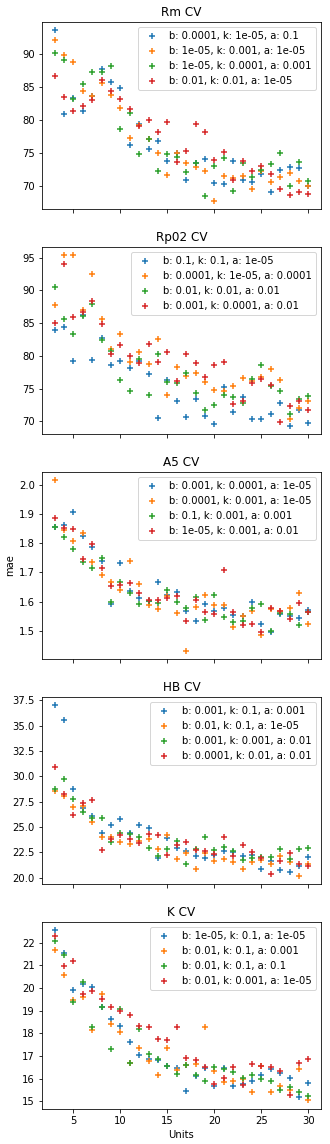
\includegraphics[width=\textwidth]{images/perf_avg_mae.png}
         \caption{MAE}
         \label{fig:perf-avg-mae}
     \end{subfigure}
     \hfill
     \begin{subfigure}[b]{0.37\textwidth}
         \centering
         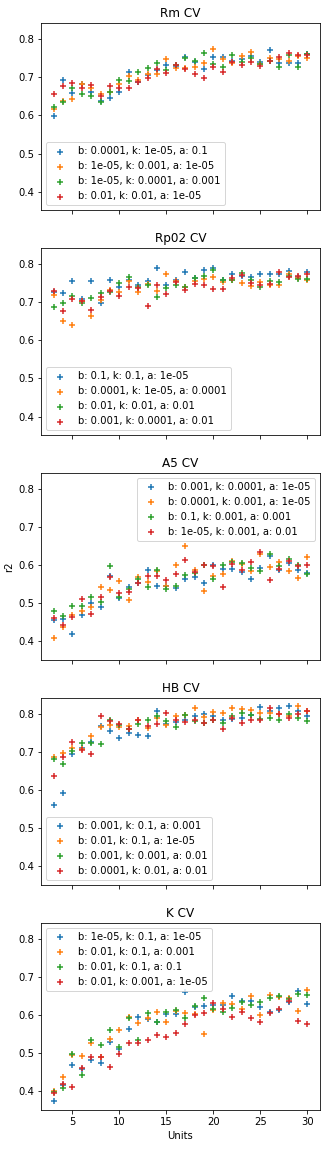
\includegraphics[width=\textwidth]{images/perf_avg_r2.png}
         \caption{$R^{2}$}
         \label{fig:peft-avg-r2}
     \end{subfigure}
        \caption{Wykres zależności jakości modelu mierzonej w metrykach: (a)średniego błędu bezwzględnego oraz (b)współczynnika determinacji od liczby neuronów w warstwie ukrytej}
        \label{fig:perf-avg}
\end{figure}

\FloatBarrier

W następnym kroku, wykorzystując dwie opracowane strategie wyboru modeli - 'avg' i 'split' (opisane w sekcji \ref{sec:ea-train}), zostały zbudowane modele komitetów sieci neuronowych, w których w skład wchodziło od 2 do 30 najlepszych modeli. Do każdej ze strategii modele wybierane były pod względem najlepszych wyników dla metryk współczynnika determinacji i średniego błędu bezwzględnego. Modele komitetów były tworzone korzystając z modeli wytrenowanych z jednego podzbioru próbek pochodzących z walidacji krzyżowej.

Analizując wykresy zależności liczby modeli od ich jakości (rys. \ref{fig:rm-committee}, \ref{fig:rp02-committee}, \ref{fig:a5-committee}, \ref{fig:hb-committee}, \ref{fig:k-committee}) można zauważyć, że zwiększanie liczby modeli poprawia jakość wyników komitetu tylko do pewnego momentu (np. na rys. \ref{fig:ea-split-mae-rm} do 10 modeli jakość się zwiększa a od 11 modeli jakość zaczyna się pogarszać). Następnie można zauważyć tendencję spadku jakości wraz ze wzrastaniem liczby modeli. Świadczy to o złym wpływie zbyt dużej liczby parametrów modelu na jakość przewidywania.

Zauważalna jest także przewaga strategii wybierania modeli spośród najlepszych modeli wytrenowanych na danym podzbiorze ze zbiorów wyznaczonych przy walidacji krzyżowej (strategia 'split'). Niewiele gorsze wyniki daje strategia wyznaczania najlepszych konfiguracji na podstawie najlepszych wyników jakości przedstawionych jako średnia ze wszystkich podziałów walidacji krzyżowej. Widoczna przy tej strategii jest mniejsza degradacja jakości przy zwiększaniu liczby modeli (rys. \ref{fig:ea-avg-r2-rp02} i \ref{fig:ea-avg-mae-rp02}).

Dokładne wyniki najlepszych komitetów zostały przedstawione w tabeli \ref{tab:committee-bests}. Dla każdej z właściwości mechanicznych zostały przedstawione 4 najlepsze komitety pod względem każdej ze strategi i metryki użytej do wyłonienia najlepszych modeli wchodzących w skład komitetu. Najlepsze wyniki dla każdej z właściwości mechanicznych zostały osiągnięte przy użyciu strategii 'split'. Liczba modeli wchodzacych w skład najlepszych komitetów nie przekraczała 5 w przypadku metryki $R^{2}$. Dla metryki MAE tylko w przypadku modelu dla właściwości Rm liczba modeli dla najlepszego komitetu wyniosła 10.

\begin{figure}
     \centering
     \begin{subfigure}[b]{0.49\textwidth}
         \centering
         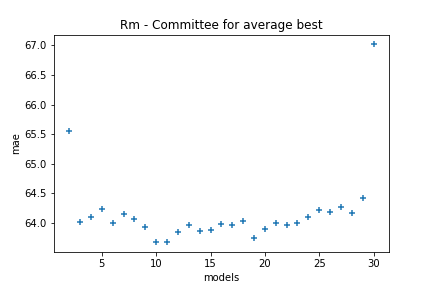
\includegraphics[width=\textwidth]{images/Rm_avg_mae.png}
         \caption{}
         \label{fig:ea-avg-mae-rm}
     \end{subfigure}
     \begin{subfigure}[b]{0.49\textwidth}
         \centering
         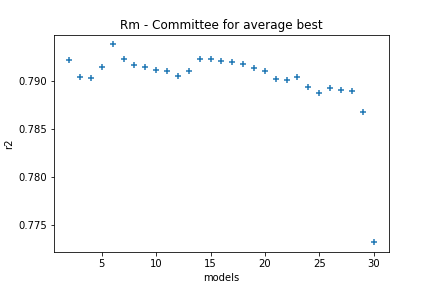
\includegraphics[width=\textwidth]{images/Rm_avg_r2.png}
         \caption{}
         \label{fig:ea-avg-r2-rm}
     \end{subfigure}
     \hfill
     \begin{subfigure}[b]{0.49\textwidth}
         \centering
         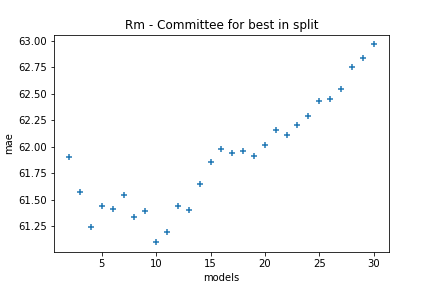
\includegraphics[width=\textwidth]{images/Rm_split_mae.png}
         \caption{}
         \label{fig:ea-split-mae-rm}
     \end{subfigure}
     \begin{subfigure}[b]{0.49\textwidth}
         \centering
         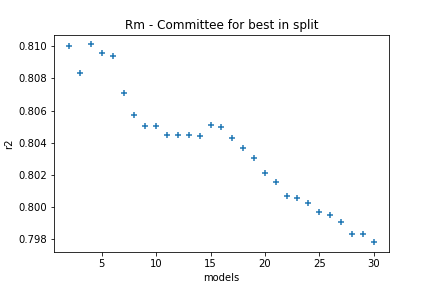
\includegraphics[width=\textwidth]{images/Rm_split_r2.png}
         \caption{}
         \label{fig:ea-split-r2-rm}
     \end{subfigure}
        \caption{Wykresy zależności jakości modelu mierzonej w metrykach: (a i c) średniego błędu bezwzględnego oraz (b i d) współczynnika determinacji od liczby modeli wchodzacych w skład komitetów (przewidujących właściwość Rm)}
        \label{fig:rm-committee}
\end{figure}

\begin{figure}
     \centering
     \begin{subfigure}[b]{0.49\textwidth}
         \centering
         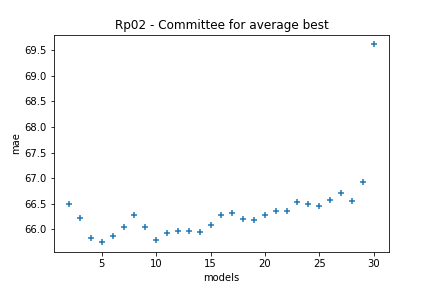
\includegraphics[width=\textwidth]{images/Rp02_avg_mae.png}
         \caption{}
         \label{fig:ea-avg-mae-rp02}
     \end{subfigure}
     \begin{subfigure}[b]{0.49\textwidth}
         \centering
         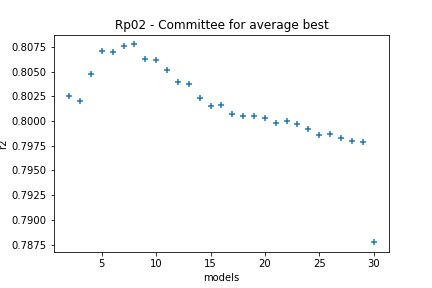
\includegraphics[width=\textwidth]{images/Rp02_avg_r2.png}
         \caption{}
         \label{fig:ea-avg-r2-rp02}
     \end{subfigure}
     \hfill
     \begin{subfigure}[b]{0.49\textwidth}
         \centering
         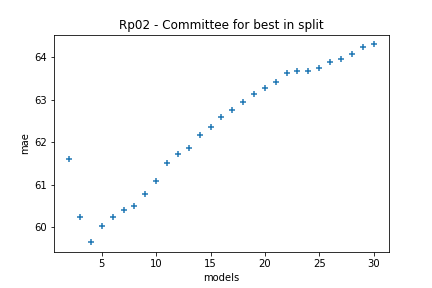
\includegraphics[width=\textwidth]{images/Rp02_split_mae.png}
         \caption{}
         \label{fig:ea-split-mae-rp02}
     \end{subfigure}
     \begin{subfigure}[b]{0.49\textwidth}
         \centering
         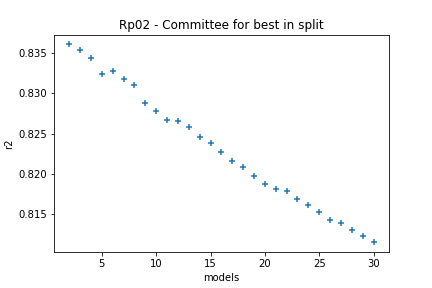
\includegraphics[width=\textwidth]{images/Rp02_split_r2.png}
         \caption{}
         \label{fig:ea-split-r2-rp02}
     \end{subfigure}
        \caption{Wykresy zależności jakości modelu mierzonej w metrykach: (a i c) średniego błędu bezwzględnego oraz (b i d) współczynnika determinacji od liczby modeli wchodzacych w skład komitetów (przewidujących właściwość Rp02)}
        \label{fig:rp02-committee}
\end{figure}

\begin{figure}
     \centering
     \begin{subfigure}[b]{0.49\textwidth}
         \centering
         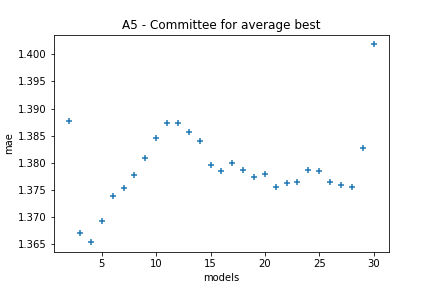
\includegraphics[width=\textwidth]{images/A5_avg_mae.png}
         \caption{}
         \label{fig:ea-avg-mae-a5}
     \end{subfigure}
     \begin{subfigure}[b]{0.49\textwidth}
         \centering
         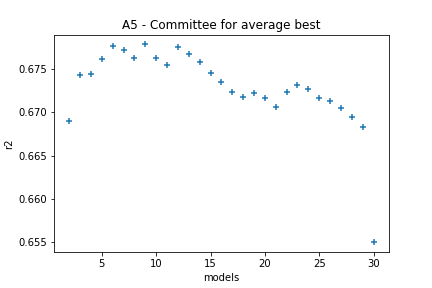
\includegraphics[width=\textwidth]{images/A5_avg_r2.png}
         \caption{}
         \label{fig:ea-avg-r2-a5}
     \end{subfigure}
     \hfill
     \begin{subfigure}[b]{0.49\textwidth}
         \centering
         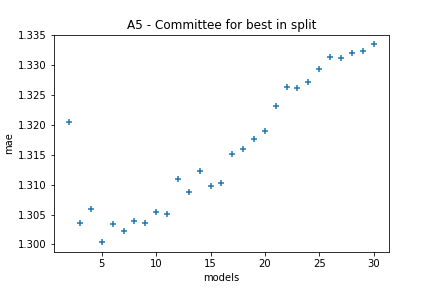
\includegraphics[width=\textwidth]{images/A5_split_mae.png}
         \caption{}
         \label{fig:ea-split-mae-a5}
     \end{subfigure}
     \begin{subfigure}[b]{0.49\textwidth}
         \centering
         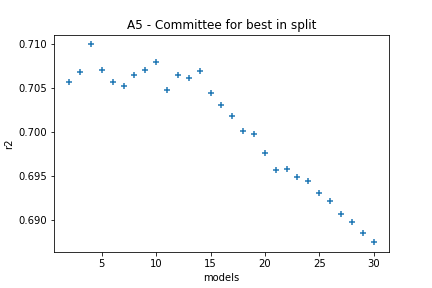
\includegraphics[width=\textwidth]{images/A5_split_r2.png}
         \caption{}
         \label{fig:ea-split-r2-a5}
     \end{subfigure}
        \caption{Wykresy zależności jakości modelu mierzonej w metrykach: (a i c) średniego błędu bezwzględnego oraz (b i d) współczynnika determinacji od liczby modeli wchodzacych w skład komitetów (przewidujących właściwość A5)}
        \label{fig:a5-committee}
\end{figure}

\begin{figure}
     \centering
     \begin{subfigure}[b]{0.49\textwidth}
         \centering
         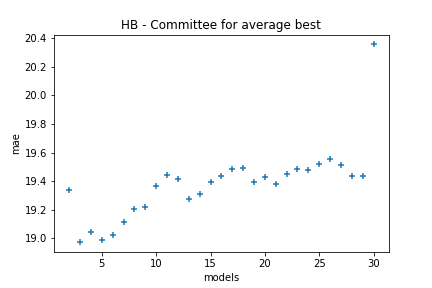
\includegraphics[width=\textwidth]{images/HB_avg_mae.png}
         \caption{}
         \label{fig:ea-avg-mae-hb}
     \end{subfigure}
     \begin{subfigure}[b]{0.49\textwidth}
         \centering
         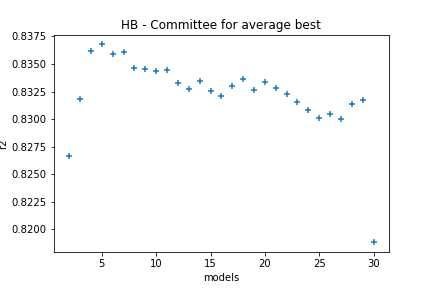
\includegraphics[width=\textwidth]{images/HB_avg_r2.png}
         \caption{}
         \label{fig:ea-avg-r2-hb}
     \end{subfigure}
     \hfill
     \begin{subfigure}[b]{0.49\textwidth}
         \centering
         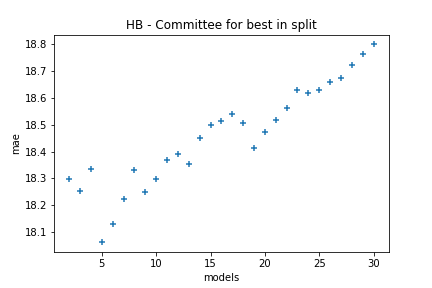
\includegraphics[width=\textwidth]{images/HB_split_mae.png}
         \caption{}
         \label{fig:ea-split-mae-hb}
     \end{subfigure}
     \begin{subfigure}[b]{0.49\textwidth}
         \centering
         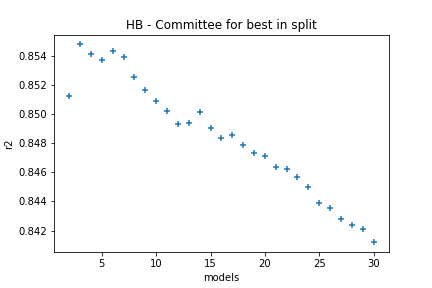
\includegraphics[width=\textwidth]{images/HB_split_r2.png}
         \caption{}
         \label{fig:ea-split-r2-hb}
     \end{subfigure}
        \caption{Wykresy zależności jakości modelu mierzonej w metrykach: (a i c) średniego błędu bezwzględnego oraz (b i d) współczynnika determinacji od liczby modeli wchodzacych w skład komitetów (przewidujących właściwość HB)}
        \label{fig:hb-committee}
\end{figure}

\begin{figure}
     \centering
     \begin{subfigure}[b]{0.49\textwidth}
         \centering
         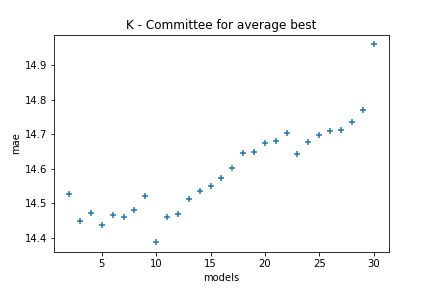
\includegraphics[width=\textwidth]{images/K_avg_mae.png}
         \caption{}
         \label{fig:ea-avg-mae-k}
     \end{subfigure}
     \begin{subfigure}[b]{0.49\textwidth}
         \centering
         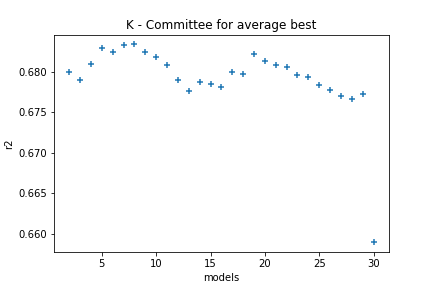
\includegraphics[width=\textwidth]{images/K_avg_r2.png}
         \caption{}
         \label{fig:ea-avg-r2-k}
     \end{subfigure}
     \hfill
     \begin{subfigure}[b]{0.49\textwidth}
         \centering
         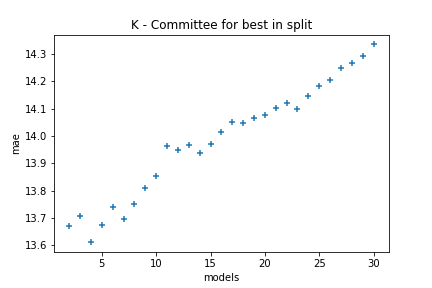
\includegraphics[width=\textwidth]{images/K_split_mae.png}
         \caption{}
         \label{fig:ea-split-mae-k}
     \end{subfigure}
     \begin{subfigure}[b]{0.49\textwidth}
         \centering
         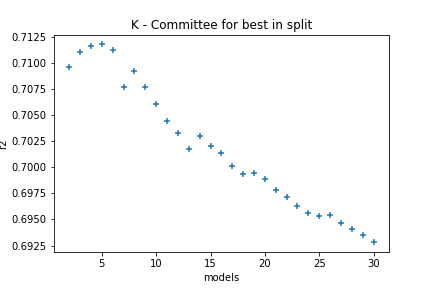
\includegraphics[width=\textwidth]{images/K_split_r2.png}
         \caption{}
         \label{fig:ea-split-r2-k}
     \end{subfigure}
        \caption{Wykresy zależności jakości modelu mierzonej w metrykach: (a i c) średniego błędu bezwzględnego oraz (b i d) współczynnika determinacji od liczby modeli wchodzacych w skład komitetów (przewidujących właściwość K)}
        \label{fig:k-committee}
\end{figure}

\FloatBarrier

\begin{table}[H]
\caption{Tabela przestawiająca najlepsze modele komitetów dla wszystkich właściwości mechanicznych z podziałem na najlepsze pod względem strategi i metryki dobierania modeli}
    \label{tab:committee-bests}
    \centering
    \begin{tabular}{|M{1cm}|M{1.5cm}|M{1.5cm}|M{1.25cm}||M{1.25cm}|M{1.25cm}|}
        \hline
        Wł. & strategia & metryka & liczba modeli & $R^{2}$ & MAE\\
        \hline
        \hline
        \multirow{4}{*}{Rm} & \multirow{2}{*}{avg} & $R^{2}$ & 6 & 0.794 & 63.594\\
        \cline{3-6}
        && MAE & 10 & 0.791 & 63.678 \\
        \cline{2-6}
        & \multirow{2}{*}{split} &$R^{2}$&4 & \textbf{0.810} & 61.533 \\
        \cline{3-6}
        && MAE & 10 & 0.804 & \textbf{61.098} \\
        \hline
        \hline
        \multirow{4}{*}{Rp02} & \multirow{2}{*}{avg} & $R^{2}$ & 8 & 0.808 & 65.402 \\
        \cline{3-6}
        && MAE & 5 & 0.802 & 65.749 \\
        \cline{2-6}
        & \multirow{2}{*}{split} &$R^{2}$&2 & \textbf{0.836} & 62.612 \\
        \cline{3-6}
        && MAE & 4 & 0.832 & \textbf{59.652} \\
        \hline
        \hline
        \multirow{4}{*}{A5} & \multirow{2}{*}{avg} & $R^{2}$ & 9 & 0.678 & 1.382 \\
        \cline{3-6}
        && MAE & 4 & 0.672 & 1.365 \\
        \cline{2-6}
        & \multirow{2}{*}{split} &$R^{2}$&4 & \textbf{0.710} & 1.320 \\
        \cline{3-6}
        && MAE & 5 & 0.701 & \textbf{1.300} \\
        \hline
        \hline
        \multirow{4}{*}{HB} & \multirow{2}{*}{avg} & $R^{2}$ & 5 & 0.837 & 18.988 \\
        \cline{3-6}
        && MAE & 3 & 0.835 & 18.974 \\
        \cline{2-6}
        & \multirow{2}{*}{split} &$R^{2}$&3 & \textbf{0.855} & 18.089 \\
        \cline{3-6}
        && MAE & 5 & 0.849 & \textbf{18.062} \\
        \hline
        \hline
        \multirow{4}{*}{K} & \multirow{2}{*}{avg} & $R^{2}$ & 8 & 0.683 & 14.732 \\
        \cline{3-6}
        && MAE & 10 & 0.686 & 14.387 \\
        \cline{2-6}
        & \multirow{2}{*}{split} &$R^{2}$&5 & 0.712 & 13.808 \\
        \cline{3-6}
        && MAE & 4 & \textbf{0.713} & \textbf{13.612} \\
        \hline
    \end{tabular}
    
\end{table}

\subsection{Porównanie jakości zbadanych modeli}\label{sec:comp-eval}
Aby dokonać oceny, które algorytmy uczenia maszynowego sprawdziły się najlepiej dla zebranych danych, w tabeli \ref{tab:best_compare} zostały przedstawione najlepsze wyniki dla poszczególnych algorytmów pod względem metryki $R^{2}$. 

Jednoznacznie można wskazać, że najlepszym algorytmem okazał się Gradient Boosting.  Osiągnął on najlepsze wyniki dla każdej z właściwości mechanicznych. Dla właściwości Rm i Rp02 dobrze sprawdził się także algorytm Ensemble Averaging, przy czym osiągnał on gorsze wyniki w pozostałych przypadkach. Największym zaskoczeniem jest wynik algorytmu Random Forest dla właściwości HB, gdzie zajął on drugie miejsce a w przypadku pozostałych właściwości plasował się na miejscach ostatnim i przedostatnim.


\begin{table}[H]
 \caption{Tabela przestawiająca zestawienie najlepszych wyników dla wszystkich użytych algorytmów dla wszystkich właściwości mechanicznych.}
    \label{tab:best_compare}
    \centering
    \begin{tabular}{|M{1cm}|M{4cm}|M{1.5cm}|}
        \hline
        Wł. & algorytm & $R^{2}$\\
        \hline
        \hline
        \multirow{4}{*}{Rm} & Gradient Boosting & 0.8243 \\
        \cline{2-3}
        & Ensemble Averaging & 0.810 \\
        \cline{2-3}
        & Random Forest &  0.8081\\
        \cline{2-3}
        & Multilayer Perceptron & 0.8011 \\
        \hline
        \hline
        \multirow{4}{*}{Rp02} & Gradient Boosting & 0.8513 \\
        \cline{2-3}
        & Ensemble Averaging & 0.836 \\
        \cline{2-3}
        & Multilayer Perceptron & 0.8287 \\
        \cline{2-3}
        & Random Forest &  0.8054\\
        \hline
        \hline
        \multirow{4}{*}{A5} & Gradient Boosting & 0.7296 \\
        \cline{2-3}
        & Random Forest &  0.7121\\
        \cline{2-3}
        & Ensemble Averaging & 0.710 \\
        \cline{2-3}
        & Multilayer Perceptron & 0.6890 \\
        \hline
        \hline
        \multirow{4}{*}{HB} & Gradient Boosting & 0.8791 \\
        \cline{2-3}
        & Random Forest & 0.8674\\
        \cline{2-3}
        & Ensemble Averaging & 0.855 \\
        \cline{2-3}
        & Multilayer Perceptron & 0.8416 \\
        \hline
        \hline
        \multirow{4}{*}{K} & Gradient Boosting & 0.7694 \\
        \cline{2-3}
        & Multilayer Perceptron & 0.7351 \\
        \cline{2-3}
        & Random Forest &  0.7230\\
        \cline{2-3}
        & Ensemble Averaging & 0.713 \\
        \hline
    \end{tabular}
   
\end{table}

\section{Badanie algorytmów optymalizacji}\label{sec:opt-research}
W tej sekcji zostały opisane badania, których celem było sprawdzenie, które z algorytmów wspomnianych w sekcji \ref{sec:algos} będą zdolne do optymalizacji kryteriów kosztu i jakości przedstawionych w postaci skalaryzacji ważonej (funkcja QC opisana w sekcji \ref{sec:opt}).

\subsection{Przygotowanie do badań}
Przeprowadzenie badań wiązało się z przygotowaniem następujących elementów:
\begin{itemize}
    \item rozwiązania początkowe, które pozwolą na ukazanie jak algorytmu poradzą sobie z przypadkami bardzo odległymi od rozwiązań optymalnych - w tym celu zostały w 300 losowych krokach wybrane 2 początkowe rozwiązania, z których jedno zostało wybrane z największą wartością funkcji kosztu a drugie z najmniejszą wartością funkcji jakości,
    \item wagi kryteriów, które ze względu na większe skomplikowanie funkcji kosztu zostały wybrane właśnie z większym uwzględnieniem tego kryterium - wagi: [koszt - 1.0, jakość 0.0], [koszt - 0.7, jakość - 0.3], [koszt - 0.5, jakość - 0.5],
    \item maksymalny czas przeszukiwania - została ustalona wartość 10 sekund,
    \item grubość wytopu - została ustalona wartość 30mm,
    \item gatunek z normy PN-EN 1564:2012 - została wybrana norma GJS-800-10,
    \item wartości parametrów od których zależy funkcja kosztu:
    \begin{itemize}
        \item średnia cena żeliwa - 1350,
        \item średnia waga wsadu - 200,
        \item koszt niklu - 16,
        \item koszt miedzi - 12,
        \item koszt molibdenu - 7.
    \end{itemize}
    \item modele właściwości mechanicznych - wybrane zostały modele wytrenowane za pomocą algorytmu XGBoost ze względu na szybkość działania.
\end{itemize}

Wybrane rozwiązania początkowe: 
\begin{itemize}
    \item Rozwiązanie z najwyższym kosztem (Rozwiązanie 1):
    \begin{itemize}
        \item skład chemiczny - [C=3.45, Si=2.48, Mn=0.4, Mg=0.05, Cu=0.3, Ni=1.5, Mo=0.5, S=0.012, P=0.013, Cr=0.0, V=0.0, CE=4.281],
        \item parametry obróbki termicznej - [aust\_temp=830, aust\_czas=60, ausf\_czas=735, ausf\_temp=430],
        \item wartość funkcji kosztu - 509136.538,
        \item wartość funkcji jakości - 31.
    \end{itemize}
    \item Rozwiązanie z najniższą jakością (Rozwiązanie 2):
    \begin{itemize}
        \item skład chemiczny - [C=3.45, Si=2.48, Mn=0.4, Mg=0.05, Cu=0.3, Ni=1.5, Mo=0.5, S=0.012, P=0.013, Cr=0.0, V=0.0, CE=4.281],
        \item parametry obróbki termicznej - [aust\_temp=835, aust\_czas=45, ausf\_czas=615, ausf\_temp=440],
        \item wartość funkcji kosztu - 466137.584,
        \item wartość funkcji jakości - 23.
    \end{itemize}
\end{itemize}

W przypadku algorytmów Tabu Search, Metropolis Search czy Parallel Tempering, przyjmują one parametry, które wpływają na ich działanie. Zostały one przetestowane w następujących konfiguracjach:
\begin{itemize}
    \item Tabu Search - rozmiar tablicy tabu z wartościami: [5, 10, 50],
    \item Metropolis Search - temperatura początkowa: [20, 50],
    \item Parallel Tempering - w przypadku tego algortmu należy podać wartości dla parametrów:
    \begin{itemize}
        \item 'num\_replicas' (liczba replik instancji algorytmu Metropolis Search),
        \item 'minTemperature'(minimalna temperatura dla nowej instacji Metropolis Search),
        \item 'maxTemperature'(maksymalna temperatura dla nowej instancji Metropolis Search).\\
        Wybrane zostały konfiguracje: 
        \begin{itemize}
            \item \{'num\_replicas':5,  'minTemperature':1, 'maxTemperature':200\},
            \item \{'num\_replicas':10,  'minTemperature':10, 'maxTemperature':100\}.
        \end{itemize}
    \end{itemize}  
\end{itemize}

Biorąc pod uwagę dwa początkowe rozwiazania, 3 różne zbiory dla wag kryteriów i 9 algorytmów (włączając tutaj różne konfiguracje dla Tabu Search, Metropolis Search oraz Parallel Tempering) proces optymalizacji został uruchomiony łącznie 54 razy.

\subsection{Wyniki badań}

Na pierwszym etapie badań został sprawdzony determinizm użytych algorytmów. W~tym celu każdy z nich został uruchomiony 10 razy z różnymi ziarnami losowości dla każdego z rozwiązań początkowych i wagach kryteriów 0.5 dla kosztu i jakości. Wyniki zostały zaprezentowane w tabeli \ref{tab:random-stability}, gdzie zostały zawarte kolumny opisujące najmniejszą i średnią wartość funkcji QC oraz jej odchylenie standardowe.

\begin{table}[H]
 \caption{Tabela przedstawiająca wyniki testu determinizmu użytych algorytmów dla każdego z rozwiazań początkowych i z wagami [koszt - 0.5, jakość 0.5]}
    \label{tab:random-stability}
    \centering
    \begin{tabular}{|M{0.5cm}|M{4.4cm}|M{1cm}|M{1cm}|M{1cm}||M{1cm}|M{1cm}|M{1cm}|}
        \hline
        \multirow{2}{*}{Lp} & \multirow{2}{*}{algorytm} & \multicolumn{3}{c||}{Rozwiązanie 1} & \multicolumn{3}{c|}{Rozwiązanie 2}\\
        \cline{3-8}
        &&min&avg&std&min&avg&std\\
        \hline
        1&TABU\_5 & 29.26 & 29.26 & 0.00&29.26 & 29.26 & 0.00\\
        \hline
        2&TABU\_10 & 29.26 & 29.26 & 0.00&29.26 & 29.26 & 0.00\\
        \hline
        3&TABU\_50 & 0.76 & 0.76 & 0.00&29.26 & 29.26 & 0.00\\
        \hline
        4&RANDOM\_DESCENT & 35.24 & 35.24 & 0.00&29.26 & 29.26 & 0.00\\
        \hline
        5&STEEPEST\_DESCENT & 29.26 & 29.26 & 0.00&29.26 & 29.26 & 0.00\\
        \hline
        6&METRO\_20 & 0.76 & 0.76 & 0.00&0.76 & 0.76 & 0.00\\
        \hline
        7&METRO\_50 & 0.93 & 0.95 & 0.01&0.96 & 0.96 & 0.00\\
        \hline
        8&PARALLEL\_5\_1.0\_200.0 & 0.76 & 17.56 & 13.26&0.98 & 12.70 & 10.82\\
        \hline
        9&PARALLEL\_10\_10\_100.0 & 1.13 & 25.58 & 11.29&29.28 & 33.73 & 3.00\\
        \hline
    \end{tabular}
\end{table}

Wyniki przedstawione w tabeli pokazują, że brak determinizmu występuje tylko dla algotymu Parallel Tempering (wiersze 8 i 9) oraz dla Metropolis Search z temperaturą początkową 50 w teście dla pierwszego rozwiązania początkowego. Niedeterminizm został stwierdzony na podstawie odchylenia standardowego wartości funkcji QC dla rozwiązań zbliżonych do optymalnych po 10 sekundach od uruchomienia algorytmów.

\subsubsection{Sposób przedstawienia dalszych wyników}
Podczas uruchamiania algorytmów, ich wyniki były zapisywane wspólnie dla uruchomień z tym samym początkowym rozwiązaniem oraz tymi samymi wagami kryteriów. Wyniki wszystkich uruchomień w takiej grupie zostały przedstawione w postaci tabelarycznej, w których znajdują się następujące kolumny:
\begin{itemize}
    \item 'algo' - nazwa algorytmu wraz z konfiguracją parametrów, przykładowo 'METRO\_50' oznacza algorytm Metropolis Search z parametrem temperatury początkowej o wartości 50,
    \item 'step' - krok algorytmu, w którym zostało znalezione najlepsze rozwiązanie,
    \item 'millis' - liczba milisekund, po których najlepsze rozwiązanie zostało znalezione,
    \item 'qce' - liczba ewaluacji funkcji QC do momentu znalezienia najlepszego rozwiązania,
    \item 'me' - liczba ewaluacji właściwości mechanicznych do momentu znalezienia najlepszego rozwiązania,
    \item 'qc' - wartość funkcji QC dla najlepszego rozwiązania.
\end{itemize}

Następnie, z każdej grupy zostało wybrane 5 najlepszych algorytmów i ich przebieg został wspólnie przedstawiony na wykresach. Osią x na wykresach jest liczba milisekund od startu, a na osi y pokazane są wartości funkcji QC.
\FloatBarrier
\subsubsection{Wyniki dla rozwiązania pierwszego z wagami [koszt - 1.0, jakość 0.0]}
W tabeli \ref{tab:opt-sol1-w1} przedstawiającej wyniki uruchomień algorytmów dla konfiguracji zawartej w tytule tej podsekcji możemy zauważyć, że ostatnie dwa algorytmy nie poradziły sobie zbyt dobrze z zadaniem optymalizacji w tym przypadku. Dwa pierwsze miejsca zajął algorytm Tabu Search z tablicą tabu o rozmiarze 10 i 50 minimalizując funkcję QC do tej samej wartości. Różnicą był tutaj czas, który był dłuższy dla drugiej konfiguracji, zapewne ze względu na więcej operacji wykonanych na większej tablicy tabu. Dodatkowo, konfiguracja z pierwszej pozycji potrzebowała najmniej czasu na znalezenie optymalnego rozwiązania. Przebiegi pięciu najlepszych konfiguracji znajdują się na rys. \ref{fig:sol-1-w-1}.
\begin{table}[H]
 \caption{Tabela przedstawiająca wyniki osiągnięte przez badane algorytmy przeszukiwania dla rozwiązania pierwszego z wagami [koszt - 1.0, jakość 0.0].}
    \label{tab:opt-sol1-w1}
    \centering
    \begin{tabular}{|M{0.5cm}|M{4.4cm}|M{1cm}|M{1cm}|M{1cm}|M{1cm}|M{1.1cm}|}
        \hline
        Lp &algo &  step & millis & qce & me & \textbf{qc}\\
        \hline
       1&TABU\_10&72&655&785&7240&1.146\\
        \hline
        2&TABU\_50&72&962&785&7240&1.146\\
        \hline
        3&METRO\_50&9139&1181&6675&9140&1.315\\
        \hline
        4&TABU\_5&57&914&697&5759&1.337\\
        \hline
        5&METRO\_20&19653&3018&13670&19654&1.349\\
        \hline
        6&STEEPEST\_DESCENT&54&846&661&5509&1.477\\
        \hline
        7&PARALLEL\_5\_1.0\_200.0&4&9273&6436&8858&1.851\\
        \hline
        8&RANDOM\_DESCENT&187&75&135&188&28.943\\
        \hline
        9&PARALLEL\_10\_10\_100.0&2&10447&7557&9945&39.526\\
        \hline
    \end{tabular}
   
\end{table}

\begin{figure}[ht]{}
	\centering
	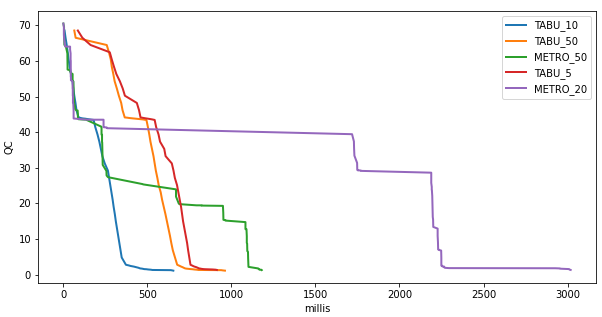
\includegraphics[scale=0.85]{images/solution_1_cqp_1.png}
	\caption {
		 Wykres przedstawiający historię przebiegu 5 najlepszych algorytmów dla rozwiązania pierwszego z wagami [koszt - 1.0, jakość 0.0]. 
	}
	\label{fig:sol-1-w-1}
\end{figure}

\subsubsection{Wyniki dla rozwiązania pierwszego z wagami [koszt - 0.7, jakość - 0.3]}
W tabeli \ref{tab:opt-sol1-w2}, przedstawiającej wyniki uruchomień algorytmów dla konfiguracji zawartej w tytule tej podsekcji, na pierwszym miejscu znajduje się algorytm Tabu Search z~tablicą tabu o rozmiarze 50. Zakończył on optymalizację w czasie 3s znajdując optymalne rozwiązanie. Takie samo optymalne rozwiązanie zostało znalezione przez algorytm Metropolis Search z temperaturą początkową o wartości 50 (pozycja druga w tabeli), jednak potrzebował on ponad 3x więcej czasu w porównaniu do Tabu Search. Na rys. \ref{fig:sol-1-w-2} zostały przedstawione przebiegi uruchomienia 5 najlepszych konfiguracji algorytmów.
\begin{table}[H]
\caption{Tabela przedstawiająca wyniki osiągnięte przez badane algorytmy przeszukiwania dla rozwiązania pierwszego z wagami [koszt - 0.7, jakość - 0.3].}
    \label{tab:opt-sol1-w2}
    \centering
    \begin{tabular}{|M{0.5cm}|M{4.4cm}|M{1.2cm}|M{1cm}|M{1cm}|M{1.2cm}|M{1.1cm}|}
        \hline
        Lp &algo &  step & millis & qce & me & \textbf{qc}\\
        \hline
        1&TABU\_50&260&3031&2350&25938&1.062\\
        \hline
        2&METRO\_50&103400&9992&72213&103401&1.062\\
        \hline
        3&METRO\_20&35568&3296&24971&35569&1.247\\
        \hline
        4&PARALLEL\_5\_1.0\_200.0&5&9605&7495&10329&5.382\\
        \hline
        5&PARALLEL\_10\_10\_100.0&2&8571&6074&8073&5.669\\
        \hline
        6&TABU\_5&32&465&311&3234&29.272\\
        \hline
        7&TABU\_10&32&321&311&3234&29.272\\
        \hline
        8&STEEPEST\_DESCENT&32&297&311&3265&29.272\\
        \hline
        9&RANDOM\_DESCENT&214&25&144&215&37.754\\
        \hline
    \end{tabular}
    
\end{table}
\begin{figure}[ht]{}
	\centering
	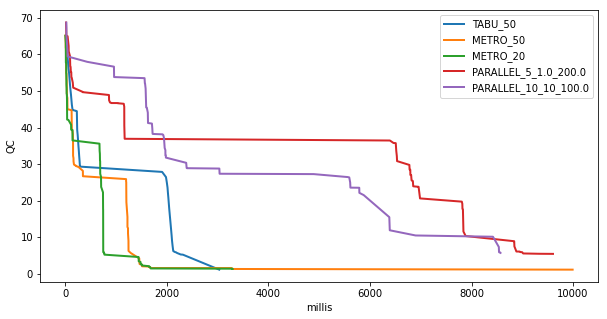
\includegraphics[scale=0.85]{images/solution_1_cqp_2.png}
	\caption {
		 Wykres przedstawiający historię przebiegu 5 najlepszych algorytmów dla rozwiązania pierwszego z wagami [koszt - 0.7, jakość - 0.3]. 
	}
	\label{fig:sol-1-w-2}
\end{figure}


\subsubsection{Wyniki dla rozwiązania pierwszego z wagami [koszt - 0.5, jakość - 0.5]}
W tej konfiguracji pierwsze miejsce ex aequo ponownie zajął algorytm Tabu Search z~tablicą tabu o rozmiarze 50 (tabela \ref{tab:opt-sol1-w3}). Zaraz za nim znajduje się algorytm Metropolis Search z temperaturą początkową o wartości 50. Ponownie, obie konfuguracje znalazły takie samo optymalne rozwiązanie z tą różnicą, że tym razem Metropolis Search był 3x szybszy. Na miejscach 3 i 4 znalazły się konfiguracje, których wyniki są bardzo zbliżone do tego optymalnego, jednak czas potrzebny na znalezienie tych rozwiązań był wielokrotnie wyższy w porównianiu do Metropolis Search z temperaturą początkową o wartości 50.
\begin{table}[H]
\caption{Tabela przedstawiająca wyniki osiągnięte przez badane algorytmy przeszukiwania dla rozwiązania pierwszego z wagami [koszt - 0.5, jakość - 0.5].}
    \label{tab:opt-sol1-w3}
    \centering
    \begin{tabular}{|M{0.5cm}|M{4.4cm}|M{1.2cm}|M{1cm}|M{1cm}|M{1cm}|M{1.1cm}|}
        \hline
        Lp &algo &  step & millis & qce & me & \textbf{qc}\\
        \hline
        1&TABU\_50&260&2993&2350&25938&0.759\\
        \hline
        2&METRO\_50&9350&862&6723&9351&0.759\\
        \hline
        3&PARALLEL\_5\_1.0\_200.0&4&7889&6621&9035&0.927\\
        \hline
        4&METRO\_20&71514&7353&49123&71515&0.968\\
        \hline
        5&TABU\_5&32&370&311&3234&29.260\\
        \hline
        6&TABU\_10&32&332&311&3234&29.260\\
        \hline
        7&STEEPEST\_DESCENT&32&364&311&3265&29.260\\
        \hline
        8&RANDOM\_DESCENT&214&27&144&215&35.319\\
        \hline
        9&PARALLEL\_10\_10\_100.0&0&3925&3551&4647&36.548\\
        \hline
    \end{tabular}
    
\end{table}

\begin{figure}[ht]{}
	\centering
	\includegraphics[scale=0.85]{images/solution_1_cqp_3.png}
	\caption {
		 Wykres przedstawiający historię przebiegu 5 najlepszych algorytmów dla rozwiązania pierwszego z wagami [koszt - 0.5, jakość - 0.5]. 
	}
	\label{fig:sol-1-w3}
\end{figure}

\subsubsection{Wyniki dla rozwiązania drugiego z wagami [koszt - 1.0, jakość 0.0]}
Wyniki tej konfiguracji (tabela \ref{tab:opt-sol2-w1}) pokazują, że najlepiej poradził sobie ponownie algorytm Tabu Search z tablicą tabu o rozmiarze 50. Czas potrzebny na znalezienie optymalnego rozwiazania wyniósł 1,5 sekundy. Na dalszych dwóch miejscach uplasował sie algorytm Metropolis Search z wynikami zbliżonymi do tego z pierwszego miejsca. 
\begin{table}[H]
\caption{Tabela przedstawiająca wyniki osiągnięte przez badane algorytmy przeszukiwania dla rozwiązania drugiego z wagami [koszt - 1.0, jakość 0.0].}
    \label{tab:opt-sol2-w1}
    \centering
    \begin{tabular}{|M{0.5cm}|M{4.4cm}|M{1.2cm}|M{1cm}|M{1cm}|M{1cm}|M{1.1cm}|}
        \hline
        Lp &algo &  step & millis & qce & me & \textbf{qc}\\
        \hline
        1&TABU\_50&97&1485&836&9675&1.147\\
        \hline
        2&METRO\_50&9138&972&6683&9139&1.315\\
        \hline
        3&METRO\_20&19652&2500&13678&19653&1.350\\
        \hline
        4&PARALLEL\_5\_1.0\_200.0&3&3975&4355&5897&1.788\\
        \hline
        5&PARALLEL\_10\_10\_100.0&4&10994&13968&18884&2.517\\
        \hline
        6&TABU\_5&42&341&357&4202&28.943\\
        \hline
        7&TABU\_10&42&372&357&4202&28.943\\
        \hline
        8&RANDOM\_DESCENT&282&30&200&283&28.943\\
        \hline
        9&STEEPEST\_DESCENT&42&1211&357&4243&28.943\\
        \hline
    \end{tabular}
    
\end{table}

\begin{figure}[ht]{}
	\centering
	\includegraphics[scale=0.85]{images/solution_2_cqp_1.png}
	\caption {
		 Wykres przedstawiający historię przebiegu 5 najlepszych algorytmów dla rozwiązania drugiego z wagami [koszt - 1.0, jakość 0.0]. 
	}
	\label{fig:sol-2-w-1}
\end{figure}

\subsubsection{Wyniki dla rozwiązania drugiego z wagami [koszt - 0.7, jakość - 0.3]}
Dla tej konfiguracji zwycięzcą poraz pierwszy okazał się algorytm Metropolis Search z~temperaturą początkową o wartości 20 (tabela \ref{tab:opt-sol2-w2}. Na drugim miejscu także znajduje się algorytm Metropolis Search ale z temperaturą początkową o wartości 50. Obie konfiguracje uzyskały takie samo rozwiązanie optymalne lecz konfiguracja z temperaturą początkową o wartości 20 znalazła to rozwiązanie w czasie krótszym o 0.4 sekundy. 
\begin{table}[H]
\caption{Tabela przedstawiająca wyniki osiągnięte przez badane algorytmy przeszukiwania dla rozwiązania drugiego z wagami [koszt - 0.7, jakość - 0.3].}
    \label{tab:opt-sol2-w2}
    \centering
    \begin{tabular}{|M{0.5cm}|M{4.4cm}|M{1.2cm}|M{1cm}|M{1cm}|M{1cm}|M{1.1cm}|}
        \hline
        Lp &algo &  step & millis & qce & me & \textbf{qc}\\
        \hline
        1&METRO\_20&35568&3459&24978&35569&1.248        \\
        \hline
        2&METRO\_50&35824&3859&24925&35825&1.248        \\
        \hline
        3&PARALLEL\_5\_1.0\_200.0&4&8335&6665&9232&5.167        \\
        \hline
        4&PARALLEL\_10\_10\_100.0&3&12910&11155&14960&20.633        \\
        \hline
        5&TABU\_5&37&302&326&3702&29.272        \\
        \hline
        6&TABU\_10&37&327&326&3702&29.272        \\
        \hline
        7&TABU\_50&37&311&326&3702&29.272        \\
        \hline
        8&STEEPEST\_DESCENT&37&311&326&3738&29.272        \\
        \hline
        9&RANDOM\_DESCENT&1066&91&598&1067&37.755        \\
        \hline
    \end{tabular}
    
\end{table}

\begin{figure}[ht]{}
	\centering
	\includegraphics[scale=0.85]{images/solution_2_cqp_2.png}
	\caption {
		 Wykres przedstawiający historię przebiegu 5 najlepszych algorytmów dla rozwiązania drugiego z wagami [koszt - 0.7, jakość - 0.3]. 
	}
	\label{fig:sol-2-w-2}
\end{figure}

\subsubsection{Wyniki dla rozwiązania drugiego z wagami [koszt - 0.5, jakość - 0.5]}
Wyniki dla tej konfiguracji (tabela \ref{tab:opt-sol2-w3}) różnią się od poprzednich. Rozwiązania zadowalające zostały znalezione tylko przez algorytm Metropolis Search z temperaturami 20 i 50, gdzie ten drugi znalazł konfigurację z mniejszą wartością funkcji QC i potrzebował na to prawie 10x mniej czasu. Pozostałe konfiguracje utkneły w minimach lokalnych. Przy większym czasie maksymalnym istnieje podejrzenie, że konfiguracje z algorytmem Tabu Search znalazłyby optymalne rozwiązania. Takie podejrzenie jest uzasadnione ze względu na dobre wyniki algorytmu Tabu Search w poprzednich badaniach.
\begin{table}[H]
\caption{Tabela przedstawiająca wyniki osiągnięte przez badane algorytmy przeszukiwania dla rozwiązania drugiego z wagami [koszt - 0.5, jakość - 0.5].}
    \label{tab:opt-sol2-w3}
    \centering
    \begin{tabular}{|M{0.5cm}|M{4.4cm}|M{1.2cm}|M{1cm}|M{1cm}|M{1cm}|M{1.1cm}|}
        \hline
        Lp &algo &  step & millis & qce & me & \textbf{qc}\\
        \hline
        1&METRO\_50&9352&731&6725&9353&0.759\\
        \hline
        2&METRO\_20&71515&6400&49128&71516&0.968\\
        \hline
        3&TABU\_5&37&365&326&3702&29.260\\
        \hline
        4&TABU\_10&37&291&326&3702&29.260\\
        \hline
        5&TABU\_50&37&453&326&3702&29.260\\
        \hline
        6&STEEPEST\_DESCENT&37&372&326&3738&29.260\\
        \hline
        7&PARALLEL\_5\_1.0\_200.0&3&8451&5368&7343&29.260\\
        \hline
        8&PARALLEL\_10\_10\_100.0&3&6515&8573&11319&32.442\\
        \hline
        9&RANDOM\_DESCENT&1066&86&598&1067&35.319\\
        \hline
    \end{tabular}
    
\end{table}

\begin{figure}[ht]{}
	\centering
	\includegraphics[scale=0.85]{images/solution_2_cqp_3.png}
	\caption {
		 Wykres przedstawiający historię przebiegu 5 najlepszych algorytmów dla rozwiązania drugiego z wagami [koszt - 0.5, jakość - 0.5]. 
	}
	\label{fig:sol-2-w-3}
\end{figure}

\subsection{Analiza wyników}
Analiza przeprowadzonych badań przynosi następujące wnioski:
\begin{itemize}
    \item algorytmy Random Descent i Steepest Descent w każdym przypadku kończyły w~minimach lokalnych i zawsze plasowały się poza pierwszą piątką,
    \item algorytm Parallel Tempering najlepsze wyniki osiągał w konfiguracji z 5 replikami i temperaturami od 1 do 200. W pierwszej piątce plasował się 4 razy, jednak w~porówaniu do konkurentów charakteryzował się dłuższym czasem potrzebnym na znalezienie rozwiązania optymalnego,
    \item algorytm Tabu Search plasował się 11 razy w pierwszej piątce, a najlepsze rozwiązania znajdował w konfiguracji z tablicą tabu o rozmiarze 50,
    \item najlepszym algorytmem okazał się Metropolis Search występując ze wszystkimi swoimi konfiguracjami w każdej najlepszej piątce. Najlepszą konfiguracją okazała się ta z temperaturą o wartości 50, która zawsze znajdowała rozwiązanie optymalne bądź bardzo zbliżone do optymalnego.
\end{itemize}

Z przeprowadzonej analizy wynika, że najlepszymi algorytmami okazały się:
\begin{itemize}
    \item Tabu Search z tablicą tabu o rozmiarze 50,
    \item Metropolis Search z temperaturą początkową o wartości 50.
\end{itemize}
Dla tych dwóch konfiguracji zostały uśrednione czasy wyszukiwania rozwiązań zbliżonych do optymalnych, liczba wywołań funkcji QC oraz liczba wywołań ewaluacji modelu właściwości mechanicznych. Wyniki zostały przedstawione w tabeli \ref{tab:algo-comp}. Wynika z nich, że algorytm Tabu Search potrzebował średnio prawie 2x mniej czasu na znalezienie rozwiazań optymalnych. W przypadku porównania średniej liczby wywołań funkcji QC, tutaj różnica jest prawie 20 krotna na korzyść algorytmu Tabu Search. Podobnie dla średniej liczby ewaluacji modelu, gdzie różnica jest tutaj około 2 krotna. Wartości w tabeli znajdujące się w nawiasach zostały obliczone bez uwzględniania wyników dla TABU\_50 z tabeli \ref{tab:opt-sol2-w3}, gdyż w tym przypadku algorytm nie zbliżył się do rozwiązania optymalnego i jego wyniki w pewnym stopniu zakłamują zebrane statystyki.

\begin{table}[H]
\caption{Tabela przedstawiająca porównanie algorytmów Tabu Search i Metropolis Search pod wzgledem średniego czasu, liczby wywołań funkcji QC oraz liczby wywołań ewaluacji modelu właściwości mechanicznych}
    \label{tab:algo-comp}
    \centering
    \begin{tabular}{|M{3cm}|M{3cm}|M{3cm}|M{3.25cm}|}
        \hline
        algo &  avgTime	&avgQcEval&	avgModelEval\\
        \hline
        TABU\_50&1539.17(2117.75)&1162.17(1580.25)&12699.17(17197.75)\\
        \hline
        METRO\_50&2932.83&20657.33&29368.17\\
        \hline
    \end{tabular}
    
\end{table}

Biorąc pod uwagę wszystkie wyniki i porównania można dojść do wniosku, że algorytm Metropolis Search będzie odpowiednim wyborem dla środowiska, w którym ewaluacja modelu właściwości mechanicznych oraz ewaluacja funkcji QC nie będą wąskim gardłem gdyż wpłynie to na liczba czasu potrzebnego na znalezienie rozwiazań optymalnych. Algorytm Tabu Search potrzebując mniej czasu oraz pamiętając jakie rozwiązania są nieoptymalne, sprawdzi się wtedy, gdy ewaluacja modeli i funkcji QC będzie bardziej kosztowna pod względem czasu.



\chapter{Podsumowanie} \label{chap:conclusions}

\section{Osiągnięte cele i obserwacje}
Celem pracy było opracowanie rozwiązania, które będzie w stanie wspomagać decyzje w odlewni żeliwa ADI. Rozwiązanie opisane w pracy jest oparte na użyciu danych pochodzących z badań nad żeliwem ADI. Dane te zostały skrupulatnie zebrane z literatury i pozytywnie ocenione przez ekspertów. Następnie został opracowany algorytm służący do uzupełnienia brakujących danych, lecz jego późne ukończenie nie pozwoliło na zastosowanie zbiorów danych przez niego uzupełnionych.

Zostały wybrane i zbadane 4 złożone algorytmy uczenia maszynowego: Random Forest, Multilayer Perceptron, Gradient Boosting i Ensemble Averaging. W wyniku przeprowadzonych badań zostały wytrenowane modele właściwości mechanicznych żeliwa ADI, a najlepszymi okazały się te wytrenowane za pomocą algorytmu Gradient Boosting.

Następnie wytrenowane modele zostały użyte ewaluacji ograniczeń nakładanych przez normę. Przestrzeń rozwiązań dla dla metaheurystycznych algorytmów optymalizacji została stworzona w oparciu o zebrany zbiór danych. Zadanie optymalizacji zostało oparte o minimalizację funkcji, która została przedstawiona jako skalaryzacja ważona kryteriów kosztu i jakości. Rozwiązania musiały także spełniać wymagania ustanowione w normie opisującej istniejące gatunki żeliwa ADI. W pracy zostały przetestowane takie algorytmy jak Hill Climbing, Stochastic Hill Climbing, Metropolis Search, Tabu Search oraz Parallel Tempering. Analiza przeprowadzonych badań dostarczyła dwie konfiguracje algorytmów, które osiągnęły najlepsze wyniki: Tabu Search z tablica tabu o rozmiarze 50 oraz Metropolis Search z temperaturą początkową o wartości 50. Wynikiem są optymalne rozwiązania składające się z parametrów składu chemicznego i obróbki termicznej żeliwa ADI spełniające wymaganą normę.

\section{Obszary rozwoju}
Według mnie w pracy istnieje potencjał na dalszy rozwój każdego z opracowanych elementów. Wydaje mi się, że możliwym jest rozszerzenie zbioru danych o dodatkowe rekordy opisujące wpływ składu chemicznego i parametrów obróbki termicznej na właściwości mechaniczne żeliwa ADI. Istnieje także możliwość usprawnienia opracowanego algorytmu uzupełniania danych, który pozwoli na zbudowanie obszerniejszych zbiorów danych. 

Następnym kierunkiem rozwoju mogłoby być użycie ewolucyjnych sieci neuronowych w celu zbudowania jeszcze lepszych modeli właściwości mechanicznych, co wydaje się możliwe przy użyciu rozszerzonych i uzupełnionych zbiorów danych.

W przypadku optymalizacji, dobrym kierunkiem według mnie byłoby opracowanie większej liczby kryteriów np. związanych ze składem chemicznym czy właściwościami mechanicznymi (określone stosunki wytrzymałości na rozciąganie do granicy plastyczności czy wydłużenia). Następnie użycie bardziej zaawansowanych algorytmów z dziedziny algorytmów metaheurystycznych.



% \cleardoublepage % to ensure that the page reference is correct
% \addcontentsline{toc}{chapter}{\listfigurename}
% \listoffigures

\nocite{*} % forces bibtex to include all citations, whether or not they were referred to in the paper

\cleardoublepage
\addcontentsline{toc}{chapter}{Bibliografia}
\bibliographystyle{bib-style}
\bibliography{bibliography}

\addcontentsline{toc}{chapter}{Załącznik}
\captionsetup{list=no}
\chapter*{Załącznik}\label{sec:zalacznik}
Ta część pracy została przeznaczona na przybliżenie działania zaimplementowanego systemu i jego interfejsu użytkownika (sekcja \ref{sec:system}). W celu uruchomienia systemu należy pobrać jego kod źródłowy z repozytorium znajdującego się pod adresem: \url{https://github.com/somas3k/casting_dss}. 
W repozytorium znajdują się następujące elementy:
\begin{itemize}
    \item katalog \textit{models} - zawiera pliki modeli wytrenowanych za pomocą algorytmu XGBoost wraz z konfiguracjami warstw wejściowych oraz plik \textit{possible\_values.json} opisujący przestrzeń rozwiązań wygenerowaną dla zbioru danych,
    \item katalog \textit{python\_analysis} - zawiera notebook jupyter o nazwie \textit{optimization\_analyze.ipynb} w którym zapisane są skrypty służące do analizy danych historycznych dla analizy algorytmów,
    \item katalog \textit{src} - zawiera pliki źródłowe programu napisanego w języku Java.
    \item \textit{pom.xml} - plis opisujący zależności projektu oraz sposób budowania wykonywalnego pliku jar.
\end{itemize}

Do zbudowania i uruchomienia projektu potrzebne są następujące elementy:
\begin{itemize}
    \item Java 11 JDK (dostępne pod adresem \url{https://www.openlogic.com/openjdk-downloads}),
    \item Apache Maven (dostępne pod adresem \url{https://maven.apache.org/download.cgi}),
    \item JavaFX 11 SDK (dostępne pod adresem \url{https://gluonhq.com/products/javafx/})
\end{itemize}

Po zaistalowaniu Java 11 i Maven'a należy się upewnić, że oba narzędzia działają. Można to zrobić poprzez wywołanie w wierszu poleceń komend \textit{java --version} i \textit{mvn --version}, które powinny zwrócić zainstalowane wersje. Jeśli wersje są inne należy doprowadzić do sytuacji, by zmienna środowiskowa PATH zawierała poprawne katalogi do plików binarnych JDK i Maven'a. W przypadku Maven'a należy także dodać zmienną środowiskową \textit{JAVA\_HOME}, która będzie wskazywała na katalog z zainstalowanym JDK.

Następnie należy wypakować JavaFX 11 SDK w dowolnym miejscu na dysku i przy pomocy wiersza poleceń przejść do katalogu z pobranym repozytorium. Z poziomu katalogu należy uruchomić polecenie \textit{mvn clean install}, które w rezultacie powinno stworzyć katalog \textit{target} i zakończyć się wiadomością typu: 'BUILD SUCCESS'.

W celu uruchomienia programu należy wywołać następujące polecenie:

\textit{java \-\-module-path \%PATH\_TO\_OPENJFX\_SDK\%/lib \-\-add-modules javafx.controls, javafx.fxml, javafx.graphics -jar ./target/casting\_dss-1.0-SNAPSHOT-jar-with-dependencies.jar}

gdzie wartość \textit{\%PATH\_TO\_OPENJFX\_SDK\%} powinna zostać zastąpiona ścieżką do katalogu z JavaFX 11 SDK, przykład:

\textit{java \-\-module-path /home/kamilw/magisterka/casting\_dss/lib/javafx-sdk-11.0.2/lib \-\-add-modules javafx.controls,javafx.fxml,javafx.graphics -jar ./target/casting\_dss-1.0-SNAPSHOT-jar-with-dependencies.jar}

Poprawne uruchomienie powinno pokazać okno programu z pierwszą otwartą zakładką (rys. \ref{fig:okno1})


\begin{figure}[ht]{}
	\centering
	\includegraphics[scale=0.8]{images/okno1.png}
	\caption {
		 Okno aplikacji z otwartą zakładką 'Konfiguracja'.
	}
	\label{fig:okno1}
\end{figure}

Zakładki 'Konfiguracja', 'Norma', 'Parametry funkcji kosztu' oraz 'Zakresy produkcyjne' służą do wprowadzenia danych wejściowych, które zostaną użyte przy optymalizacji.

Najbardziej rozbudowaną częścią systemu jest zakładka 'Uruchamianie algorytmu', której stan początkowy wygląda jak na rys. \ref{fig:initial-state}.

\begin{figure}[ht]{}
	\centering
	\includegraphics[scale=0.48]{images/initial_state.png}
	\caption {
		 Okno aplikacji z otwartą zakładką 'Uuchamianie algorytmu'.
	}
	\label{fig:initial-state}
\end{figure}

W górnej części okna można zauważyć szereg przycisków. Ich działanie jest następujące:
\begin{itemize}
    \item Wygeneruj losowe - tablica pod rzędem przycisków zostanie wypełniona losowym rozwiązaniem (rys. \ref{fig:random_solution}),
    \item Usuń - usuwa dane z tablicy z rozwiązaniem,
    \item Zapisz - pozwala zachować rozwiązanie tymczasowo w pamięci,
    \item Przywróć - przywraca rozwiązanie, które zostało wcześniej zapisane za pomocą poprzedniego przycisku,
    \item Wprowadź - naciśnięcie tego przycisku skutkuje otwarciem się okna do wprowadzenia swojego rozwiązania (rys. \ref{fig:input}).
    
\end{itemize}

\begin{figure}[ht]{}
	\centering
	\includegraphics[scale=0.6]{images/random_solution.png}
	\caption {
		 Tablica przedstawiająca aktualne rozwiązanie.
	}
	\label{fig:random_solution}
\end{figure}

\begin{figure}[ht]{}
	\centering
	\includegraphics[scale=0.6]{images/input.png}
	\caption {
		 Dialog do wprowadzania rozwiązania.
	}
	\label{fig:input}
\end{figure}

Tablica wyświetlająca aktualny wynik posiada też możliwość wprowadzania zmian po naciśnięciu na wybrane pole.

Dla rozwiązania widniejącego w tablicy są wyświetlane informacje o: Cenie, Jakości, wartości Rm, Rp02, A5, HB i K (rys. \ref{fig:data-view}).

\begin{figure}[ht]{}
	\centering
	\includegraphics[scale=0.7]{images/data.png}
	\caption {
		 Kontrolki do wyświetlania informacji o koszcie, jakości i wartościach właściwości mechanicznych dla rozwiązania w tabeli.
	}
	\label{fig:data-view}
\end{figure}

W części przedstawionej na rysunku \ref{fig:algo-config} znajdują się kontrolki służące do konfiguracji czasu przeszukiwania, wybrania algorytmu i uruchomienia optymalizacji.

\begin{figure}[ht]{}
	\centering
	\includegraphics[scale=0.7]{images/algo_config.png}
	\caption {
		 Konfiguracja uruchamiania algorytmu optymalizacji.
	}
	\label{fig:algo-config}
\end{figure}

Po naciśnięciu przycisku 'Uruchom' wybrany algorytm rozpocznie optymalizację i w polu tekstowym u dołu okna zaczną się pojawiać informacje o nowych rozwiązaniach, które będą także wpisywane do tabeli z rozwiązaniem. Przykładowy 'log' został przedstawiony na rys. \ref{fig:algo-log}. Przycisk 'Zatrzymaj' służy do zatrzymania działania algorytmu optymalizacji przed upływem maksymalnego czasu przeszukiwania, a przycisk 'Wyczyść log' służy do wyczyszczenia pola tekstowego z logami.

\begin{figure}[ht]{}
	\centering
	\includegraphics[scale=0.7]{images/algo_log.png}
	\caption {
		 Logi wypisywane podczas procesu optymalizacji.
	}
	\label{fig:algo-log}
\end{figure}



\end{document}

